% !TeX spellcheck = en_US
\documentclass[11pt, a4paper]{article}
% --- Paquetes Esenciales para Idioma y Fuentes ---
\usepackage[utf8]{inputenc}
\usepackage[T1]{fontenc}
\usepackage[english]{babel} % Cambiar a spanish si el texto es en español

% --- Paquetes de Matemáticas y Símbolos (Corrige el error \blacktriangleleft) ---
\usepackage{amsmath, amsfonts,amssymb}
%\usepackage{amsfonts}
%\usepackage{amssymb}
\usepackage{url}
\usepackage{graphicx}
\usepackage{xcolor} % Necesario para los colores
\usepackage{caption} % <--- PAQUETE FUNDAMENTAL
% Configuración global para que TODOS los captions multilínea se centren:
\captionsetup{justification=centering}
% --- Paquetes para Listas Avanzadas (Corrige el error leftmargin=*) ---
\usepackage{enumitem}

% --- Paquetes para Tablas Avanzadas (Corrige los errores de \toprule y tabularx) ---
\usepackage{booktabs}
\usepackage{tabularx}
\usepackage{array}

% --- Configuración de Márgenes Estándar ---
\usepackage[margin=1in]{geometry}
\usepackage{ragged2e}

%\usepackage{enumitem}
%\usepackage{tabularx}
%\usepackage{booktabs}
%\usepackage{amssymb}
\usepackage{tikz}
\usetikzlibrary{mindmap}
\usetikzlibrary{arrows.meta}
\usetikzlibrary{positioning}
\usepackage{mathrsfs}
\usepackage{pgfplots}     % <--- CARGA EL PAQUETE DE GRÁFICAS
\pgfplotsset{compat=1.18} % <--- DEFINE LA COMPATIBILIDAD DE EJES

\title{Abstract modeling: a possible interpretation from formal reduction to praxis interpretation for renewable Power Systems}

\author{José González de Durana $^{1,*}$}



%\address[$^{1}$]{%
%Department of Systems Engineering and Automation (Professor Emeritus), University of the Basque Country (UPV/EHU), Nieves Cano 12, 01006 Vitoria-Gasteiz, Spain; jose.gonzalezdedurana@ehu.eus, jmgdurana@gmail.com}


%\address[$^{1}$]{%
%Department of Systems Engineering and Automation, University of the Basque Country (UPV/EHU), Nieves Cano 12, 01006 Vitoria-Gasteiz, Spain; jose.gonzalezdedurana@ehu.eus, jmgdurana@gmail.com}

%\corres{Correspondence: jose.gonzalezdedurana@ehu.eus}


\begin{document}
\maketitle

\begin{abstract}
The abstract modeling workflow is then examined across major philosophical traditions, including Thomistic Scholasticism and Eastern systems of thought, such as Theravāda Abhidhamma and Neo-Confucian Li-Shi dialectics. Through this comparative analysis, the paper demonstrates a persistent cross-cultural isomorphism characterized by the omnipresence of the cyclical \textit{Regressus-Progressus} procedural loop, which serves as a universal rational mechanism linking material interaction with formal abstraction across both Western and Eastern thought. Particular emphasis is placed on Gustavo Bueno’s Philosophical Materialism (PM) as the primary adopted framework, which rigorously reformulates this ancestral circularity into a contemporary philosophy of science. By leveraging the Theory of Categorical Closure and the core mechanism of Systematic Synthetic Identity, the paper demonstrates how the human operating subject is neutralized when independent operational courses converge into an objective scientific truth. While this article firmly establishes a formal connection between Systems Theory and Philosophical Materialism (ST-PM), it explicitly emphasizes that research submissions leveraging alternative, diverse computational methodologies are highly welcome within this Special Issue. The pragmatic utility of this philosophical quality-control blueprint is validated through multidisciplinary case studies encompassing mechanical, chemical, and basic electrical systems. Finally, the developed gnoseological framework is applied directly to the modeling of renewable power systems, where the rising integration of direct current (DC) architectures allows for a nice, direct structural abstraction. By applying the principle of Synthetic Identity, traditional second-order electrical circuit variables ($V, I, R, L, C$) are restricted and projected onto an autonomous, first-order mathematical category named ``Power Dynamics'' ($P, \eta$). This translation establishes a formal categorical closure through the creation of a virtual, emergent element termed $H_{bus}$. A sufficient collection of interconnected components is developed to allow the conversion of many physical DC electrical grids into this streamlined power domain. Practical multi-agent simulation examples demonstrate how this approach provides critical operational advantages, offering superior tractability for real-time dynamic analysis and streamlined anomaly detection when grids face discrete contingencies, faults, or cyber-physical events.

\vspace{0.5cm}
\noindent \textbf{Keywords:}
abstract modeling; philosophical materialism; theory of categorical closure; synthetic identity; regressus-progressus loop; systems theory; DC microgrids; power dynamics category; H-bus emergence; cyber-physical security.
\end{abstract}

\section*{Introduction}

In this article, the term “abstract modeling” refers to a type of modeling that involves creating an abstract, simplified representation of a system or process, eliminating complicated and unnecessary details to focus on its fundamental characteristics and general behavior. The philosophical and epistemological study of this type of modeling is systematically addressed in subsequent sections within the framework of Scholasticism and Philosophical Materialism, while also referring to certain important Eastern philosophies.



However, this is not the only type of abstract modeling; many other groups coexist with entirely different meanings—though these are computational in nature rather than philosophical. For instance, Symbolic Mathematical Modeling (Julia Language tools) \cite{ma2021modelingtoolkit}, Object-Oriented Modeling (UML) \cite{rumbaugh2004uml}, Data Modeling (Conceptual Schemas) \cite{chen1976entity}, Business Process Modeling (BPMN) \cite{omg2013bpmn202}, Cognitive and Behavioral Modeling (Psychology) \cite{farrell2018computational}, Abstract Observational Modeling (Bandura) \cite{bandura1986social}, etc. This wide variety and fragmentation can make it difficult for engineers to select the most appropriate modeling path for a specific application. Nevertheless, each approach undoubtedly possesses excellent qualities for its respective application and is, of course, eligible for inclusion in this Special Issue (see also Section \ref{sec:taxo}).

Beyond these practical selection challenges, however, lies a deeper epistemological concern. In the author's opinion, it is not enough for a model to “work” on a computer; it is imperative to understand what transformations physical reality undergoes during its translation into a device-independent mathematical language. This is precisely where analytical-critical philosophy becomes a first-order engineering tool. To rigorously establish this connection, this review paper is structurally anchored around the three core dimensions explicitly declared in its title: (1) the fundamental nature of the modeling process, (2) the gnoseological boundaries of abstraction, and (3) the pragmatic application for renewable Power Systems.

The first two dimensions explore the intuitive, historical, and philosophical roots of material representation. The manuscript details how the baseline meaning of modeling has evolved from everyday practical-intuitive human culture to the ancient Mesopotamian cartographic cuneiform tablets, which represent the earliest historical systems modeling. Abstraction is subsequently dissected through the lens of Systems Theory and classical philosophy, mapping the universal presence of the analytical-synthetic Regressus-Progressus procedural loop across Western scholasticism, Paduan Renaissance logic, Theravāda Abhidhamma cognitive psychology, and Neo-Confucian Li-Shi dialectics. This cross-cultural isomorphism culminates in the adoption of Gustavo Bueno's Philosophical Materialism (PM) and the Theory of Categorical Closure. Through these frameworks, the paper details how the active human operating subject is neutralized when heterogeneous material operations converge into a Systematic Synthetic Identity, distilling objective truth within an immanent scientific category.

While these initial blocks establish the conceptual and philosophical groundwork, the third dimension applies this framework directly to a pressing, contemporary technological realm: renewable power systems. From an ontological perspective, characterizing them does not require a descriptive inventory of their disparate physical components (such as photovoltaic strings or wind turbine electronics), but rather a structural abstraction of their underlying electrical network.

This paper argues that modern renewable energy systems are fundamentally characterized by a paradigm shift toward Direct Current (DC) distribution networks. This technological transition is structurally driven by the native continuous-current operation of solar cells, chemical energy storage systems (BESS) \cite{EnergiesBESS2026}, and green hydrogen electrolyzers \cite{EnergiesElectrolyzer2026}. Furthermore, while contemporary wind farms still predominantly operate on Alternating Current (AC) internal grids, the long-term sector trajectory is also pivoting toward DC collection architectures \cite{Musasa2017Review}, a movement further consolidated by the widespread adoption of industrial high-voltage DC (HVDC) transmission links \cite{EnergiesHVDC2025}.


By defining the direct current network as the determinant context of the so-called \emph{Power Dynamics} category (see \ref{sec:pseudolinear}), traditional second-order circuit-level variables $(V, I, R, L, C)$ can be restricted and projected onto a simplified first-order power domain governed strictly by power variables and efficiency metrics $(P, \eta)$. This gnoseological translation achieves a true categorical closure through the formulation of a virtual, emergent element termed the Hybrid Bus ($H_{bus}$) as Section \ref{sec:pseudolinear} shows.

Ultimately, while the mathematical formulations and component collection developed in this review are tailored to exploit the direct structural abstraction of DC grids, they provide a foundational control-engineering blueprint whose principles regarding power flow reduction could be straightforwardly adapted and extended to alternating current (AC) power systems, as Section \ref{sec:future} alludes.

The successive sections of this paper are organized to progressively unfold these three interrelated axes, demonstrating how philosophical rigor transforms engineering design from blind statistical data-fitting into a powerful tool for transient analysis and cyber-physical anomaly detection.




\subsection*{The meaning of modeling} \label{sec:meaning}

To rigorously address the subject indicated in the title, it is essential to understand the semantics of its core concept: abstract modeling. Our first impulse may well be to turn to the dictionary. We can look up both ``Modeling'' and ``Model''. In the Oxford Dictionary, modeling (referring to systems) is defined as the work of making a simple description of a system or a process that can be used to explain it or to calculate what might happen. However, it also refers to making models of objects or the work of a fashion model.

Meanwhile, a Model is described as a simple description of a system, used for explaining how something works or calculating what might happen, but also as a copy of something, usually smaller than the original object, or a particular design or type of product, among others.

From this, two conclusions can be drawn: on the one hand, the distinct meanings of ``modeling'' and ``model'', and on the other, that \textit{a model is only an aspect}—or perhaps the object—of a broader \textit{Modeling Process}.

Then, if modeling is a process in which the model is somehow involved, the true roots of modeling should be found. We shall seek them within the practices of ancient civilizations, as well as in the intuitive idea of it—shaped by our everyday usage—that are maintained across cultural and historical contexts.

On the other hand, the qualifier ``abstract'' is more elusive, requiring its roots to be sought in philosophy. Within this framework, abstraction constitutes a circular concept closely tied to the terms Regressus and Progressus. Ubiquitous in medieval Scholasticism, these concepts were later recast in the 20th century by Gustavo Bueno within the framework of Philosophical Materialism (PM). Similar notions can also be found in various Eastern traditions, such as those of China and India.

With all of this in mind, the objective of this paper is to forge a concept of abstract modeling based on these historical and philosophical antecedents. The mind map in Figure \ref{fig:mindmap} illustrates these ideas.
\begin{figure}[h]
\centering
% Asegúrate de tener definido el color navy en tu preámbulo si lo usas, por ejemplo:
\definecolor{navy}{RGB}{0,32,96}
\begin{tikzpicture}[
mindmap, concept color=orange!30,
% Todo el texto y las uniones usarán el azul marino
every node/.style={concept, execute at begin node=\hskip0pt, text=navy, font=\bfseries},
% Raíz: Borde azul marino grueso, fondo amarillo clarito
root concept/.append style={concept color=orange!30, text=navy, fill=yellow!20, line width=2pt, font=\large\bfseries, minimum size=1cm, inner sep=0ex},
% Nivel 1: Configuración de colores y ángulos
level 1 concept/.append style={concept color=orange!30, font=\bfseries, fill=orange!20, text=navy},
% Nivel 2: Fondo rojo/crema pastel muy clarito
level 2 concept/.append style={concept color=red!30, fill=red!20, font=\small\bfseries},
grow cyclic,
level 1/.style={sibling angle=90, level distance=4cm},
level 2/.style={sibling angle=45, level distance=3.3cm},
]
\node[root concept] {Abstract Modeling}
child [concept color=red!30]{ node[level 1 concept] {Early practices} }
child [concept color=red!30]{ node[level 1 concept] {\small Practical-intuitive modeling} }
child [concept color=red!30]{ node[level 1 concept] {Philosophy}
child [concept color=red!30]{ node[level 2 concept] {\scriptsize Other philosophies} }
child [concept color=red!30]{ node[level 2 concept] {\scriptsize Philosophical Materialism} }
child [concept color=red!30]{ node[level 2 concept] {\scriptsize Eastern philosophies} }
child [concept color=red!30]{ node[level 2 concept] {\scriptsize Scholastic Philosophy} }
}
child [concept color=red!30]{ node[level 1 concept] {Systems Theory\,} };
\end{tikzpicture}
\caption{Mental map of the Abstract Modeling idea}
\label{fig:mindmap}
\end{figure}



It should be noted that while this work adopts Philosophical Materialism, researchers may frame the modeling workflow within alternative conceptual frameworks depending on their regional or academic background. As illustrated in the \textit{Philosophy} branch of the mental map in Figure~\ref{fig:mindmap}, major traditions---ranging from Scholasticism to Eastern philosophies---natively share and integrate the processual notion of the \textit{Regressus-Progressus} loop.

The option of not adopting an explicit philosophical framework is also completely valid. Scientific activities are intrinsically embedded in a unique cultural context and regional background shaped by localized philosophical traditions---such as Western scholasticism, Sinitic dialectics, or Eastern analytical thought---which directly influence the language, reasoning, and engineering methodologies employed by modelers. The fundamental notion and practical experience of this causal loop are deeply rooted in ordinary language and everyday human culture across all regions. These are realms in which individuals, regardless of their geopolitical or ancestral heritage, constantly alternate between abstract reflection and material interaction.

Next, the mind map topics are developed.


\section{Practical-intuitive modeling} \label{sec:intuitive}

While defining exactly what a model is can be difficult, everyone has an intuitive grasp of the concept and its purpose, having used one at some point—such as a house plan or a dress pattern. In this way, a \textit{model} can be described as a \textit{physical structure} that \textit{stores} \textit{relevant information} about a real-world \textit{object}.

Depending on the specific type of model, the physical structure where the data are stored varies significantly: it can consist of paper pieces, geometric curves, 3D surfaces, or interconnected material shells. Furthermore, this structural substrate can remain entirely static, undergo parametric variations based on a baseline configuration, or, in the most sophisticated scenarios, be generated dynamically on the fly as real-time physical measurements are captured. Relevant information means some \textit{abstraction} is made on the object to acquire the interesting data, discarding the other. Also, the practical utility and application of the model can be different, ranging from replicating the physical asset multiple times, to predicting the temporal behavior of the system, or even building outer envelopes and structural shells for the object, as classically exemplified in haute couture fashion architecture.







\subsubsection*{Modeling Process approach}

It should be noted that what usually is called ``the model'' is the result of an approach consisting of a sequence of trial-and-error which is described as follows with the help of the diagram in Figure \ref{fig:modeling1}. This Figure  shows the said \emph{Modeling Process approach} using the \textit{Progressus} and \textit{Regressus} transitions, borrowed from Scholastic Philosophy (see Section \ref{sec:scholastic}).

\begin{figure}[h]
\begin{center}
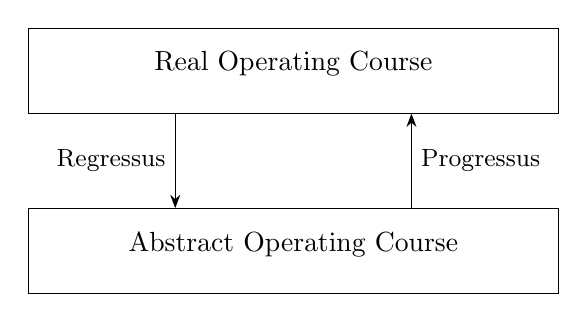
\begin{tikzpicture}[>=Stealth]
% Regressus -- Progressus
\node (box1) [draw, rectangle, text width=6.5cm, align=center]
{ \\ Real Operating Course\\ ~};
\node (box2) [below=1.2cm of box1, draw, rectangle, text width=6.5cm, align=center]
{\\ Abstract Operating Course \\~};
\draw[->, transform canvas={xshift=-1.5cm}] (box1) -- node[left] {\small Regressus} (box2);
\draw[->, transform canvas={xshift=1.5cm}] (box2) -- node[right] {\small Progressus} (box1);
\end{tikzpicture}
\end{center}\vspace{-3ex}
\caption{Modeling Process approach}
\label{fig:modeling1}
\end{figure}


The process begins in the first phase (Real Operating Course) with an object $O$, placed somewhere in the real world, waiting to be modeled. Through an appropriate measurement technique made by an operating subject or agent $A$, relevant information data $I_1$ are extracted from it. Then the Regressus transition shifts the process to the second phase (Abstract Operating Course), where the previously obtained information elements $I_1$ are managed by $A$, either arranging them within a pre-existing structure hypothetically associated with the object, or using them to construct on the fly a new structure $S_1$ to embed them. The resulting element formed by information $I_1$ structured in $S_1$ is denoted $P_1$ and it serves as the first element in a sequence of patterns or models of the real object $O$, as follows.

After $P_1$ is made, the Progressus transition sends the process back to the Abstract Operating Course phase, where $A$ assesses how well the model $P_1$ fits the object $O$  (this is sometimes referred to as model validation). This evaluation yields one of two outcomes: a satisfactory fit or an unacceptable one.

In the first case, the sequence concludes and $P_1$ becomes the definitive model. In the second case, the information elements $I_1$ must be corrected to $I_2$, after which the process continues with a new Regressus transition to make a new model $P_2$, and so on, producing in this way a sequence of models
\[
P_1, P_2, P_3, \ldots, P_n
\]
until a final model, $P_n$, is accepted.

Once the process concludes and the model $P_n$ is accepted—becoming the definitive model—the agent $A$ ceases to act; that is, it can be said that the operating subject $A$ becomes segregated from the modeling process.

So modeling has always been an active loop: a retreat from the Reality object (\textit{Regressus}) to isolate a structure (\textit{pattern or model}), followed by a synthetic return (\textit{Progressus}) to fit and compare it with the real object. This operational dynamics highlights that modeling is not a passive mirror of reality, but an active gnoseological process made by some operating agent.

The following section (\ref{haute_couture}) contains a highly instructive example  of the described process, in the Haute Couture area,  in which all its elements can be observed in detail. Later, Section \ref{sec:pmregprog} presents an explanation of the Modeling Process within the framework of Philosophical Materialism and in Section \ref{astro_example} another example in the Astronomy area is described.



\subsection{Haute couture example} \label{haute_couture}


The modeling process described above is easily verifiable in traditional garment making, because it exhibits striking structural parallels with our systematic modeling framework, thereby clarifying complex conceptual foundations, such as the ``art of modeling'' \cite{morris1967art}, discussed in systems literature. To illustrate this, the section details an example from the craft of a renowned haute couture designer, which yields profound insights. Specifically, the technical praxis of Cristóbal Balenciaga---one of the most prominent designers of the twentieth century---is examined here as a paradigmatic case.

Through the evaluation of specialized literature, historical archives, and documentary records~\cite{arzalluz2010balenciaga,dirix2022balenciaga}, his architectural craft---or rather, his structural art---can be thoroughly deconstructed. It is worth saying that this analogy encompasses virtually every main gnoseological element featured in this article, especially the bidirectional \textit{regressus-progressus} loop and the segregation of the operating subject, an intricate epistemological concept that becomes remarkably transparent through the lens of high-sartorial design.

Widely regarded as the ``architect'' and engineer of haute couture, Balenciaga revolutionized the 20th-century silhouette by prioritizing volume, geometry, and pure lines over the body's restrictions. His absolute technical mastery earned him the respect of contemporaries like Christian Dior, who called him ``the master of us all,'' and Coco Chanel, who stated he was the only true \textit{couturier} capable of designing, cutting, and sewing a dress \textit{with his own hands}.

His modeling process was a purely three-dimensional, architectural, and sculptural act. Unlike other designers of his era who captured static ideas on paper, the Basque couturier understood garments in direct relation to space and movement. Balenciaga used a cheap, provisional cotton canvas called \textit{toile} or \textit{calico} to directly capture and store the client's physical shapes. The couturier himself recorded technical data directly onto the fabric. For instance, the \textit{toile} for Mod{\`e}le 396 (F{\'e}vrier 1967) features precise handwritten notes specifying the designated workspace (\textit{Atelier Ginette}) and the house model's name (\textit{Mannequin Val{\'e}rie}), as detailed in the exhibition catalogue \cite{museoband2025catalogo}, and which has been reproduced in Figure~\ref{fig:balenciagam396} with the permission of the Cristóbal Balenciaga Foundation.


\begin{figure}[h]
\centering
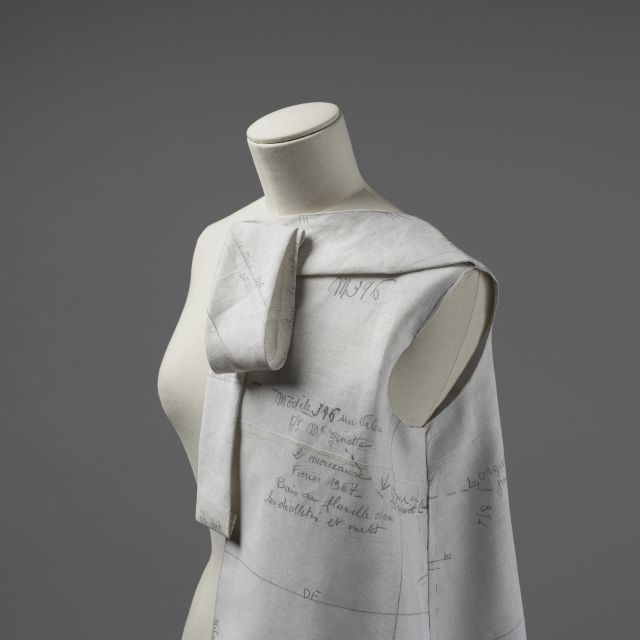
\includegraphics[width=0.4\linewidth]{figures/Balenciaga_M396}
% Es muy recomendable añadir el título corto [] para el índice de figuras (List of Figures)
\caption[Balenciaga Toile of Modèle 396.]{Balenciaga Toile of Modèle 396.\\ © Manuel Outumuro / Cristóbal Balenciaga Museoa. Getaria (Spain)}
\label{fig:balenciagam396}
\end{figure}








His rigorous methodology was structured into four operational phases:

\begin{enumerate}
\item {Dialogue with the fabric:} everything began with selecting the material. Balenciaga never forced fabrics; instead, he meticulously observed and handled them, allowing their natural weight and drape to dictate the design. His obsession with structural rigidity led him to co-develop unique textiles, such as silk gazar---a tightly woven fabric that functioned almost like a building material.

 \item {Moulage (direct draping):} the core of his genius lay in sculpting directly on the mannequin or a live model. Unlike designers who relied on paper, Balenciaga used a cheap, provisional cotton canvas called \textit{toile} or \textit{calico} to directly capture and store the client's physical shapes.
\begin{itemize}
\item {Drape control:} he rigorously marked contour lines (bust, waist, hips) on the mannequin to manipulate the canvas, controlling the grain, cross-grain, and bias to the millimeter.
\item {Air as an element:} the master draped by calculating the void---the physical space between the body and the dress---allowing the garment to create its own independent silhouette.
\end{itemize}
\item {From volume to abstract pattern:} once the perfect drape was achieved, the pins were removed, and the modeled fabric was laid flat on a table to draft the definitive patterns. Balenciaga's patterns were renowned for being deeply abstract and geometric; at first glance, it was virtually impossible to identify the placement of a neckline or armhole due to their innovative, asymmetrical cuts.

\item {The haute couture fitting protocol:} with the definitive pattern established, a new \textit{toile} was custom-tailored to the client's exact measurements. While standard houses automated this stage, the standard protocol at the Maison Balenciaga required a rigorous process structured around three regulatory fitting sessions:
\begin{itemize}

\item {The first fitting (the canvas):} the client tried on a rough prototype made of unbleached cotton \((\textit{toile}),\) pre-adjusted onto a mannequin customized to her precise body dimensions. This session defined the initial proportions, the volume relative to the body, and the overall architecture of the piece.

\item {The second fitting (basted real fabric):} after dismantling the initial \textit{toile}, the workshop cut the definitive textile (silk, wool, or gazar). The client tried on the garment held together solely by preliminary basting threads. The hang of the shoulders and the movement of the skirt were millimetrically adjusted to analyze how the material reacted in motion.

\item {The third fitting (final adjustments):} the garment was almost entirely sewn, barring closures, hems, or final trimmings. This served as the definitive verification before sewing the official house label and delivering the work.

\end{itemize}
\end{enumerate}

To ensure the structural integrity of this workflow, the fitting process under Balenciaga's supervision operated under strict epistemological and behavioral ``laws.'' First, \textit{absolute silence} was mandatory; the master communicated exclusively through subtle gestures, requiring clients to remain completely motionless while he evaluated the ``air'' between fabric and skin. Second, clients were strictly \textit{prohibited from being accompanied}, ensuring that external opinions did not contaminate the artistic and spatial dialogue between the couturier, the textile, and the body.

Yet, this protocol was governed by an absolute reset mechanism: if Balenciaga detected a defect invisible to the untrained eye, or if the fabric failed to exhibit the exact ``plumb'' (\textit{aplomo}) he demanded, he would order the garment to be completely deconstructed. This forced the entire cycle of fittings to restart from the beginning, regardless of the client's social status. Finally, once approved, this three-dimensional geometry was transferred to the final luxury fabric, incorporating concealed internal reinforcements (such as bias-cut buckram) that allowed the garment to maintain its ``floating'' volume without relying on restrictive traditional corsetry.


\subsubsection*{Analogy with the Modeling Process approach}

The comparison between Balenciaga's creative process and the Modeling Process approach described in Section \ref{sec:intuitive} is straightforward.

The \textit{Real Operating Course} phase of the diagram in Figure~\ref{fig:modeling1} would correspond to the workshop where the seamstresses crafted the dresses and models, including the \textit{Toiles}, while the \textit{Abstract Operating Course} phase would correspond to the fitting room.

The couturier usually conducted three fittings for models $P_1$, $P_2$, and $P_3$, or more if he deemed it necessary. The information elements $I_1, I_2, \ldots$ would be seen as conforming pieces of the \textit{toile}, initially pinned together and subsequently topstitched until progressively achieving the shape of each successive model $P_1, P_2, \ldots$, ultimately reaching the definitive $P_n$. One can imagine that the \textit{Regressus} and \textit{Progressus} transitions were scheduled by the master depending on the garments' manufacturing times and the business schedules.
The segregation of the operating subject is so clear in here: once the $P_{n}$ model is accepted, the client owns it and the designer's task finishes.


Perhaps the most complex element to comprehend within this example is the \textit{model} or \textit{pattern}, materialized here through the \textit{toile}. When contrasted with the intuitive description provided in Section~\ref{sec:intuitive}, this case represents the most highly sophisticated scenario: the model or pattern is physically embodied by the \textit{toile}, which the master drapes and shapes directly onto the client's body.

In standard modeling processes, an object's dimensions are typically measured using physical instruments and subsequently projected onto a formal structure, such as a geometric curve that remains static or varies strictly within a defined parametric family (e.g., an ellipse scaled by width or length). But, within Balenciaga's performance, geometric profiles were not recorded as independent numerical measurements to be later drafted onto a paper pattern or provisional fabric. Instead, the designer executed both operations simultaneously in a highly precise yet demanding manual operation: manipulating the raw cotton canvas directly; he leveraged its inherent, predictable properties of rigidity, weight, and drape to actively contour and defined the structural boundaries of the client's body.

Consequently, the toile fabric directly captures the anatomical morphology without requiring numerical data; the structural information that such measurements would normally provide is registered directly by the textile at the precise moment of the fitting, using strategically placed pins to lock and store the shape. It is, therefore, a genuinely ``on the fly'' structure that adaptively evolves each time the client undergoes a new session.



\section{Early practices}

But the said operational or technical nature of modeling is not a modern computation-driven invention: it is as old as civilization itself. The earliest concrete manifestations of abstract modeling emerged simultaneously in the pristine engineering practices of \textrm{Ancient Egypt} and \textrm{Mesopotamia}. In these early hydraulic and architectural societies, modeling did not serve a purpose of artistic contemplation. For instance, Mesopotamian master builders used cuneiform clay tablets to draw precise geometric city maps and architectural site plans.

These clay tablets contain highly valuable information, representing the earliest conceptualization not merely of a blueprint (the technical drawing) but of a complete modeling process and its intrinsic relationship with the \textit{regressus-progressus} method of scholastic philosophy. Rather than serving as passive drafts, these artifacts constitute a vestige of the birth of process modeling techniques.

% Definición paramétrica de los 5 trazos vectoriales independientes
% Horizontal: Cabeza a la izquierda, cola a la derecha (con la nueva proporción)
\newcommand{\cuniHorizontal}{%
	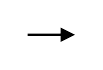
\begin{tikzpicture}[scale=0.15, baseline=-0.2ex, rotate=-90]
		\fill (0,0) -- (-0.6,-1.2) -- (-0.1,-1.2) -- (-0.1,-4) -- (0.1,-4) -- (0.1,-1.2) -- (0.6,-1.2) -- cycle;
	\end{tikzpicture}%
}
% Trazo base (Vertical): Cabeza realzada (ancho 0.6, profundidad -1.2)
\newcommand{\cuniVertical}{%
	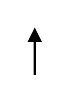
\begin{tikzpicture}[scale=0.15, baseline=-1.2ex]
		\fill (0,0) -- (-0.6,-1.2) -- (-0.1,-1.2) -- (-0.1,-4) -- (0.1,-4) -- (0.1,-1.2) -- (0.6,-1.2) -- cycle;
	\end{tikzpicture}%
}
% Diagonal Descendente: Cabeza arriba-izquierda, cola abajo-derecha
\newcommand{\cuniDiagDown}{%
	
\begin{tikzpicture}[scale=0.15, baseline=1ex, rotate=135]
		\fill (0,0) -- (-0.6,-1.2) -- (-0.1,-1.2) -- (-0.1,-4) -- (0.1,-4) -- (0.1,-1.2) -- (0.6,-1.2) -- cycle;
	\end{tikzpicture}%
}
% Diagonal Ascendente: Cabeza abajo-izquierda, cola arriba-derecha
\newcommand{\cuniDiagUp}{%
	
\begin{tikzpicture}[scale=0.15, baseline=-2ex, rotate=45]
		\fill (0,0) -- (-0.6,-1.2) -- (-0.1,-1.2) -- (-0.1,-4) -- (0.1,-4) -- (0.1,-1.2) -- (0.6,-1.2) -- cycle;
	\end{tikzpicture}%
}
% Winkelhaken: Proporción ideal a 1.2x (según lo acordado)
\newcommand{\cuniWinkel}{%
	
\begin{tikzpicture}[scale=0.15, baseline=-0.4ex]
		\fill (0,0) -- (1.44,0.84) -- (0.96,0) -- (1.44,-0.84) -- cycle;
	\end{tikzpicture}%
}



\subsubsection*{The five basic strokes of cuneiform writing}

In the cuneiform writing system, ancient Mesopotamian scribes pressed the triangular tip of a reed stylus into wet clay to create five fundamental wedge shapes. Every complex logogram, phonogram, and determinative is constructed using a combination of these five basic strokes:

\begin{description}
	\item \textrm{(\textit{A\v{S}}) Horizontal Wedge } \raisebox{0.6ex}{\cuniHorizontal}\; Created by pressing the stylus from left to right along the writing line. It is one of the most common foundational elements.

	\item \textrm{(\textit{DI\v{S}}) Vertical Wedge } \raisebox{1.6ex}{\cuniVertical}\; Created by pressing the stylus from top to bottom. It frequently acts as a number one (\textrm{1}), an itemizer for lists, or a determinative before masculine personal names.

	\item \textrm{(\textit{DI\v{S} ten\^{u}}) Downward Diagonal Wedge  \raisebox{0.6ex}{\cuniDiagDown}\; } An oblique stroke tilted at roughly a 45-degree angle, with the triangular head pointing toward the upper-left and the tail extending toward the lower-right.

	\item \textrm{(\textit{GE$_{22}$}) Upward Diagonal Wedge } \raisebox{0.6ex}{\cuniDiagUp}\;  An oblique stroke running in the opposite direction of the downward diagonal, tilted so the wedge head points toward the lower-left and the tail extends toward the upper-right.

	\item \textrm{(\textit{U}) Winkelhaken / Hook Wedge } \raisebox{0.6ex}{\cuniWinkel}\;  A short, wide, triangular arrowhead shape resembling a less-than sign ($<$). Unlike the other four strokes, it lacks an elongated tail. It is made by pressing the angular tip of the stylus obliquely into the clay and represents the number ten (\textrm{10}) or the vocalic phonogram \textit{``u''}.
\end{description}



\subsection{The Umma House}

Among the most fascinating archaeological evidence of Sumerian domestic architecture are the house plans of Umma. One of these is a clay tablet dated to the period of the Third Dynasty of Ur (approximately between 2100 and 2000 BC), which is preserved in the Vorderasiatisches Museum of Berlin in Germany under the reference VAT 7031 \cite{ummaur3}.

The plan shows the design of a Mesopotamian courtyard house featuring 7 rooms and covering approximately 114 square meters. It is so specific that, as some studies suggest, its measurements could have successfully matched those of actual archaeological findings.

\begin{figure}
	\centering
	
\includegraphics[trim={30mm 32mm 90mm 115mm}, clip, width=0.5\textwidth]{figures/Umma_house}
	\caption{Umma House}
	\label{fig:ummahouse}
\end{figure}



Ordering the 7 stanzas in lexicographic order (from left to right and from top to bottom), the annotations of the figure correspond to the original measurements of the Umma tablet, with the interpretation of the meaning of the symbols as follows:

\medskip\noindent
1. Upper Row (The roof stays)\\
-  Room 1 (Upper Left): 2 wedges ($\top\ \top$). Meaning: Write down a simple whole number (2). In the context of this perimeter room of the floor, it indicates one of the smaller dimensions of the room measured in cubits (kúš).\\[1ex]
- Room 2 (Upper Right): 3 combined wedges ($\vdash\ \top\ \blacktriangleleft$).
Meaning: It is a typical compound notation of an elongated space. The Winkelhaken represents 10; the vertical wedge is 1 and the horizontal wedge acts as a divisor or fraction mark. The scribe is indicating a long measurement (such as 11 or 13 cubits) to define the path of that upper horizontal section. \\[1ex]
2. Middle row (The middle body of the house)\\
-Room 3 (Left Hallway/Living Room): Vertical series of 4 wedges in column.
Meaning: Since it is the longest room in the plan (it covers the entire central and lower left height), the text is written in column from top to bottom. It does not represent a single number, but the complete record of the stay: Length × Width. The wedges indicate successive measurements (for example, 3 cubits wide in one section and a long extension in the other).\\
- Room 4 (Wide Central Courtyard): 3 mixed wedges with a Winkelhaken.
Meaning: It is the largest and most important room in the house. The Winkelhaken ($\blacktriangleleft$) means 10, and being accompanied by vertical wedges, it represents a generous distance (for example, 12 cubits long). It is the space that articulates the access to rooms 1, 5 and 6. \\
- Room 5 (middle, Narrow Right Wing): 2 wedges ($\top\ \blacktriangleleft$).
Meaning: Being a narrow room in a 2:1 ratio with respect to the courtyard, the wedges here register a smaller dimension for the width (usually 5 cubits, which is equivalent to about 2.5 meters, the standard for secondary or storage rooms in Umma houses).

\medskip\noindent
3. Bottom Row (The base of the plane)\\
- Room 6 (wide Central Lower): 2 wedges ($\top\\vdash$).
Meaning: Being directly connected to the courtyard (room 4), the text of room 6 defines the passage space to the exterior exit of the plane. Its wedges represent a dimension identical in width to that of the upper courtyard, maintaining the symmetry of the central block.\\
- Room 7 (lower Right Narrow): 1 horizontal wedge ($\vdash$). Meaning: In the lower corner, the scribe reduced the annotation to the minimum. A single horizontal wedge used to be used in Umma field inventories and plans to denote ``Fraction'' or ``Half a unit'' (half a cubit), or it functioned as a calculation residue of the next room (room 6) to indicate that they shared the same dividing wall.


The 7-room floor plan mathematically replicates this accounting system: the rooms with the most wedges or ten wedges coincide with the large open spaces (such as Patio 4 or living room 2), while the narrow rooms on the right (5 and 7) carry much smaller and more compact annotations.





\begin{figure}[htbp]
\centering
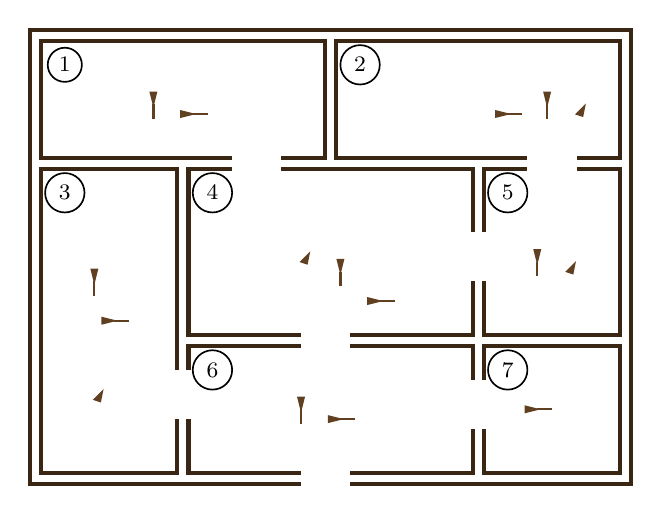
\begin{tikzpicture}[scale=1.25,
% Definición de grosores para lograr la fusión perfecta de muros dobles
muro_fondo/.style={draw=brown!30!black, line width=5.5pt, line cap=rect},
muro_interior/.style={draw=white, line width=2.5pt, line cap=rect},
door/.style={draw=white, line width=6pt}, % Máscara para abrir los huecos de las puertas
cuneiform/.style={draw=brown!50!black, fill=brown!50!black, line width=0.6pt}
]

% Macros para las cuñas cuneiformes (2 parámetros: coord X, coord Y)
\newcommand{\wedgeV}[2]{% Cuña Vertical
	\path[cuneiform] (#1,#2) -- ++(-0.03,0.12) -- ++(0.06,0) -- cycle;
	\draw[cuneiform, line width=0.8pt] (#1,#2) -- ++(0,-0.15);
}
\newcommand{\wedgeH}[2]{% Cuña Horizontal
	\path[cuneiform] (#1,#2) -- ++(-0.12,0.03) -- ++(0,-0.06) -- cycle;
	\draw[cuneiform, line width=0.8pt] (#1,#2) -- ++(0.15,0);
}
\newcommand{\wedgeD}[2]{% Winkelhaken (diagonal)
	\path[cuneiform] (#1,#2) -- ++(0.08,0.08) -- ++(-0.02,-0.1) -- cycle;
}

% ==========================================================
% CAPA 1: TRAZO GRUESO OSCURO (Fondo de todos los tabiques)
% ==========================================================
\begin{scope}[muro_fondo]
	% Marco exterior
	\draw (0,0) rectangle (6.0, 4.5);
	% Muro horizontal superior (Fila Superior)
	\draw (0, 3.2) -- (6.0, 3.2);
	% Muro horizontal inferior (Fila Central / Inferior)
	\draw (1.5, 1.4) -- (6.0, 1.4);
	% Muro vertical superior (División Hab 1 y 2)
	\draw (3.0, 3.2) -- (3.0, 4.5);
	% Muro vertical izquierdo (Límite Hab 3)
	\draw (1.5, 0.0) -- (1.5, 3.2);
	% Muro vertical derecho (Proporción 2:1)
	\draw (4.5, 0.0) -- (4.5, 3.2);
\end{scope}

% ==========================================================
% CAPA 2: TRAZO BLANCO INTERIOR (Vacía los cruces automáticamente)
% ==========================================================
\begin{scope}[muro_interior]
	% Replicamos exactamente el mismo esqueleto geométrico
	\draw (0,0) rectangle (6.0, 4.5);
	\draw (0, 3.2) -- (6.0, 3.2);
	\draw (1.5, 1.4) -- (6.0, 1.4);
	\draw (3.0, 3.2) -- (3.0, 4.5);
	\draw (1.5, 0.0) -- (1.5, 3.2);
	\draw (4.5, 0.0) -- (4.5, 3.2);
\end{scope}

% ==========================================================
% CAPA 3: APERTURA DE PUERTAS SOLICITADAS
% ==========================================================
\begin{scope}[door]
	\draw (2.0, 3.2) -- (2.5, 3.2);   % Puerta [1-4]
	\draw (5.0, 3.2) -- (5.5, 3.2);   % Puerta [2-5]
	\draw (1.5, 0.6) -- (1.5, 1.1);   % Puerta [3-6]
	\draw (2.7, 1.4) -- (3.2, 1.4);   % Puerta [4-6]
	\draw (4.5, 2.0) -- (4.5, 2.5);   % Puerta [4-5]
	\draw (4.5, 0.5) -- (4.5, 1.0);   % Puerta [6-7]
	\draw (2.7, 0.0) -- (3.2, 0.0);   % Puerta [6-exterior (abajo)]
\end{scope}
% ==========================================================
% CAPA 4: GRABADOS CUNEIFORMES REPOSICIONADOS
% ==========================================================
\wedgeV{1.2}{3.8} \wedgeH{1.6}{3.7}                   % Habitación 1
\wedgeH{4.8}{3.7} \wedgeV{5.2}{3.8} \wedgeD{5.5}{3.7}       % Habitación 2
\wedgeV{0.6}{2.0} \wedgeH{0.8}{1.6} \wedgeD{0.6}{0.8}       % Habitación 3
\wedgeD{2.7}{2.2} \wedgeV{3.1}{2.1} \wedgeH{3.5}{1.8}       % Habitación 4
\wedgeV{5.1}{2.2} \wedgeD{5.4}{2.1}                   % Habitación 5
\wedgeV{2.7}{0.7} \wedgeH{3.1}{0.6}                   % Habitación 6
\wedgeH{5.1}{0.7}                                     % Habitación
% Números de las habitaciones
\node[draw, semithick, minimum size=0.2cm, inner sep=2pt,  circle]
   	at(0.3,4.2){\footnotesize 1};
\node[draw, semithick, minimum size=0.5cm, inner sep=2pt, circle]
   	at(3.3,4.2){\footnotesize 2};
\node[draw, semithick, minimum size=0.5cm,inner sep=2pt,  circle]
	at(0.3,2.9){\footnotesize 3};
\node[draw, semithick, minimum size=0.5cm,inner sep=2pt,  circle]
	at(1.8,2.9){\footnotesize 4};
\node[draw, semithick, minimum size=0.5cm,inner sep=2pt,  circle]
	at(4.8,2.9){\footnotesize 5};
\node[draw, semithick, minimum size=0.5cm, inner sep=2pt, circle]
	at(1.8,1.1){\footnotesize 6};
\node[draw, semithick, minimum size=0.5cm,inner sep=2pt,  circle]
	at(4.8,1.1){\footnotesize 7};
\end{tikzpicture}
	\caption{Geometric layout and cuneiform codification of the complete system.}
	\label{fig:tablet_layout}
\end{figure}




\subsection{Regressus -- Progressus in Sumerian cartography}

The cognitive dynamic embedded within this tablet operates on two scales, mirroring the classic scholastic and materialist epistemological circuits.

The Sumerian clay tablets represent an early form of complete systems modeling rather than a passive architectural drawing, viewed through the lens of Scholastic Philosophy. The process involves a Progressus phase that abstracts physical terrain into formal geometric data, followed by a Regressus phase where this abstract model returns to the physical world to govern and dictate actual construction.
\subsubsection*{The Regressus phase: from the material to the formal (abstraction)}
The process originates within the empirical, physical realm. Sumerian builders and surveyors initially confronted raw matter: the irregular topography adjacent to the Euphrates, measuring reeds (\textit{gi}), cords, and mud bricks.
\begin{itemize}[leftmargin=*]
	\item The \textit{Regressus} phase occurs as the scribe abstracts this complex physical reality, elevating it into a superior formal category: the geometric model.
	\item By pressing the reed into the clay, the scribe segregates the accidental variables of the terrain (such as dust and topographical relief) and encodes space into pure lines and additive numerical cuneiform. Consequently, an intelligible model is constructed---a formalized truth that no longer depends on physical presence on the terrain.
\end{itemize}



\subsubsection*{The Progressus phase: the determinant return to matter}
It is at this stage that the tablet demonstrates it is a complete model rather than a merely descriptive map. The blueprint was not created to remain static within the clay; it was designed to return to the world and transform it.

\begin{itemize}[leftmargin=*]
	\item The \textit{Progressus} process is executed when builders employ this compact tablet as a directive norm in the actual terrain.
	\item The abstract model---representing the seven rooms in geometric order and their respective doors---returns to the material world to impose its law. It determines where the physical mud-brick walls will be erected, where the structural thresholds will open, and how light will distribute within the courtyard. Ultimately, the geometric model encoded in the clay constrains and governs the physics of the material bodies that will inhabit the house.
\end{itemize}

% =========================================================================
% NUEVA SECCIÓN: REGRESSUS-PROGRESSUS AND FEEDBACK LOOPS
% =========================================================================

\section{Systems Theory} \label{sec:systh}

A profound structural and operational isomorphism exists between the scholastic \textit{Regressus-Progressus} method and the concept of feedback within modern control systems theory. Although separated by centuries and distinct technical vocabularies, both frameworks describe the same phenomenon: a closed-loop causal circuit wherein the outcome of an action returns to its source to regulate, correct, or determine subsequent operations.

\begin{figure}
	\centering
	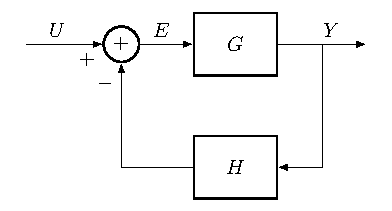
\includegraphics[width=0.36\linewidth]{figs_tikz/control_system}
	\caption{Control System}
	\label{fig:controlsystem}
\end{figure}


The divergence is not structural, but epistemological. While scholasticism and its extension into contemporary Philosophical Materialism (see the next Section)
frames this cycle in terms of ontology and epistemology (how human praxis comprehends and transforms reality), cybernetics and modern systems engineering—pioneered by figures like Norbert Wiener—formalize it mathematically to regulate dynamic physical systems. Analysed in parallel, their functional equivalence reveals a striking conceptual symmetry:

\subsection{Structural and Systems Theory paradigms}
These paradigms analyze abstraction through the lens of systemic architecture, emergent organization, and the invariant laws of complex networks.

\begin{itemize}
	\item \textrm{General Systems Philosophy (Ervin Laszlo and Von Bertalanffy) \cite{vonbertalanffy1968general}: grounded in Laszlo's \textit{Introduction to Systems Philosophy} \cite{laszlo1972introduction}}, this framework shifts from reductionist paradigms to a synthetic, holistic model of reality. Abstraction is defined here as the invariant relational structures (such as self-stabilizing cybernetic loops or open-system phase transitions) that remain mathematically constant across physical, biological, and sociological strata.
	\item \textrm{Hierarchical Systems Theory (Koestler's Holism) \cite{koestler1967ghost}}: This paradigm models complex architectures as nested hierarchies of ``holons''---entities that operate under a dual ontological nature, behaving simultaneously as autonomous whole systems looking downward, and as dependent, abstract parts looking upward.
	\item \textrm{The Viable System Model (Stafford Beer's Cybernetics): \cite{beer1985diagnosing}} An abstract organizational paradigm that maps any viable system (be it a biological brain, an enterprise, or an economy) into five invariant, abstract subsystems dedicated to operation, coordination, control, intelligence, and overarching policy.
\end{itemize}


\subsection{Taxonomy of Abstract Modeling paradigms} \label{sec:taxo}

Aside from the epistemological and ontological dimensions of abstraction analyzed in the following Section, several computational paradigms for abstract modeling coexist in practice. The following taxonomy categorizes these frameworks, establishing structural links between pragmatic computer science architectures, formal mathematical logic, and complex systems theory. Consequently, research submissions leveraging these diverse computational methodologies are highly welcome within this Special Issue.


\subsubsection*{Computability and language-driven paradigms}
These paradigms operate on a pragmatic and computational level, treating abstraction as a functional mechanism to manage complexity, isolate implementation details, and enforce structural safety in execution environments.
\begin{itemize}
	\item \textrm{Multiple Dispatch and Parametric Polymorphism (The Julia Language Paradigm) \cite{juliaparadigm}:} in high-performance computing architectures like the Julia language, abstraction is defined by decoupling data structures from behavior. Functions are abstractly declared across open, generic type signatures. The concrete modeling realization is resolved dynamically at runtime based on the full combination of the arguments' types. This fundamentally shifts the ontology of a system's entities from ``what they are'' (traditional Object-Oriented paradigms) to ``how they interact with others''.
	\item \textrm{Abstract Data Types (ADTs) and Algebraic Specification \cite{guttag_adts_algebraic}}: pioneered in formal computer science, this framework defines objects strictly by the axiomatic operations that can be performed upon them and the mathematical invariants they preserve, completely independent of their underlying physical memory representation.
	\item \textrm{Denotational Semantics (The Scott-Strachey Paradigm) \cite{stoy1977denotational}:} a formal mathematical modeling framework wherein the semantic ``meaning'' of a computational program or complex system is abstracted into pure mathematical objects (domains and continuous functions). It addresses the ontological nature of a system by mapping structural syntax directly onto abstract mathematical entities.
\end{itemize}

\subsubsection*{Formal logical and Neo-Logicist paradigms}
These paradigms approach abstraction as a rigorous formal operation that generates new, higher-level entities (abstract objects) from equivalence relations between existing entities.
\begin{itemize}
\item \textrm{The Neo-Logicist Hierarchy (Burgess's General Theory and Fine's GA+) \cite{burgess2005fixing}}: represented by John P. Burgess (\textit{Fixing Frege}) and Kit Fine (\textit{The Limits of Abstraction} \cite{fine2002limits}), this paradigm formalizes abstraction via explicit \textit{Abstraction Principles}. By systematically mapping equivalence relations on properties to identities between abstract objects, they construct an $n$-th order hierarchy of mathematical abstractions, providing a foundational ontology for structuralism and set theory.

\item \textrm{Category Theory and Topos Theory (The Grothendieck-Mac Lane Paradigm)\cite{maclane1992sheaves}}: the pinnacle of mathematical abstraction. Rather than defining entities by their internal components or foundational sets, Category Theory models complex systems entirely through ``Arrows'' (Morphisms) and relational mappings. An entity within this paradigm is ontologically defined exclusively by how it maps to and from all other objects within its universe.
\end{itemize}


\subsubsection*{Domain-specific scientific abstraction}
\begin{itemize}
	\item \textrm{Model-Theoretic Realism (The Semantic View of Theories): \cite{suppe1989semantic}} Advocated by contemporary philosophers of science, this paradigm dictates that scientific theories do not consist of linguistic or syntactic laws, but rather of a collection of abstract mathematical models that are isomorphic (or homeomorphic) to specific structures of the empirical world.
	\item \textrm{Coarse-Graining and Effective Field Theories (EFT): \cite{hartmann2001effective}} A highly rigorous paradigm derived from theoretical physics. Instead of modeling a system at its microscopic, data-heavy level, it systematically ``smooths out'' or integrates out microscopic degrees of freedom to generate an abstract, higher-level mathematical model that accurately governs macroscopic phenomena.
\end{itemize}



\subsection{The Art of Modeling in systems literature}

It is interesting to note that classic authors in systems modeling, such as Peter Wellstead \cite{Wellstead79} and François Cellier \cite{cellier1991continuous}, approach modeling not as a static mathematical algorithm, but as a living, circular praxis, often described as an ``art'' or a specialized technical craft. For these authors, modeling requires three mandatory stages that form a closed iterative loop: data acquisition from a process (\textit{System Identification}), structural fitting (\textit{Modeling}) followed by an empirical feedback with reality (\textit{Validation}).

Both Wellstead and Cellier explain that modeling cannot rely solely on theoretical imagination; it requires performing experiments on a physical process to acquire its dynamic variables and input/output data in either the time or frequency domain (System Identification). This operational requirement directly matches the concepts of \textit{Phenomenal Praxis} and \textit{Determinant Context} established within the Theory of Categorial Closure in Philosophical Materialism.

Even older publications, such as William T. Morris's essay \textit{On the Art of Modeling} \cite{morris1967art}, explain that modeling operates as an ``art'' because no unique recipe exists to determine which variables to discard and which to preserve. The modeler requires practical experience and intuition to simplify the system enough to ensure mathematical tractability, while maintaining the necessary fidelity to preserve its material truth during the validation phase.

The parallel between this technical workflow of contemporary researchers and the operational tasks performed by Mesopotamian scribes is evident.



Anticipating briefly the concepts detailed in the subsequent Philosophy section, it can be stated that by crossing this engineering loop with Gustavo Bueno's framework, the engineer's praxis mirrors the core gnoseological mechanisms of Philosophical Materialism. This closed iterative loop maps directly onto three fundamental operational phases:


\begin{enumerate}
    \item {Phenomenal praxis (System Identification):} The researcher performs a physical intervention on the real material system to acquire dynamic variables in either the time or frequency domain. This stage constitutes the active manipulation of terms within a determinant context, where physical experiments force the system to yield raw empirical data streams.
    \item {Formal Regressus (System Modeling):} The raw data streams are filtered and embedded into an abstract mathematical structure, such as differential equations, bond graphs, or state-space matrices. Here, the modeler neutralizes the secondary physical contingencies of matter, moving backward from the chaotic data points to isolate its formal essence in the $M_3$ domain.
    \item {Compositive Progressus (Validation and Verification):} The abstract model is evaluated against new experimental data sets that were not used during the modeling phase. Its objective validity does not rely on simple conceptual coherence; it is established only when the model returns to the material field ($M_1$) and demonstrates that it governs the physical phenomena. When the numerical simulation trajectories and the laboratory telemetry converge, the Systematic Synthetic Identity emerges.
\end{enumerate}

It should be noted that the sections developed thus far---\textit{Intuitive Ideas}, \textit{Early Practices}, and \textit{Systems Theory}---have only addressed the foundational meaning of the term \textit{Modeling}. However, the qualifying adjective \textit{Abstract} restricts and complicates this concept, introducing a determinant dimension that necessitates the analytical tools of Philosophy.


\section{Philosophy}

In what follows, the conceptual framework of abstract modeling is developed across consecutive sections. We begin by analyzing the Scholastic tradition and the three degrees of abstraction formulated by St. Thomas Aquinas (ST). This layout provides the necessary contrast for the subsequent section, which delineates Gustavo Bueno's Philosophical Materialism (PM) and its radical, non-idealistic reconstruction of the abstract modeling process. Finally, a discussion on Eastern philosophies is also presented.

% =========================================================================
% PARTE 1: LA BASE ESCOLÁSTICA Y EL TRÁNSITO LÓGICO HASTA PADUA
% =========================================================================


\subsection{Scholastic Philosophy} \label{sec:scholastic} \label{sec:stabstraction}

In the 13th century, the realist gnoseology of \textrm{Thomas Aquinas (ST)} postulated that the human intellect possesses no innate contents; rather, knowledge always derives from the sensible world. The key mechanism is \textrm{abstraction} (\textit{abstractio}), an operation by which the \textrm{active intellect} strips the particular and sensible image (the \textit{phantasm}) of its individual and material conditions, extracting the universal essence captured by the \textrm{possible intellect}~\cite{aquinas_st_gnoseology}.


Following the Aristotelian ontological tradition~\cite{aristotle_metaphysics}, Thomas Aquinas divides abstraction into \textrm{three formal degrees} according to the criteria established in his treatise \textit{In De Trinitate}~\cite{aquinas_de_trinitate}, depending on the level of separation from matter carried out by the intellect:
\begin{itemize}
	\item \textrm{First Degree (Physical Abstraction):} The mind disregards individual matter (this specific body, this particular animal) but retains \textrm{common sensible matter} (the material body in general, endowed with physical qualities and motion). This gives rise to Physics or the Philosophy of Nature, which studies material substances insofar as they are subject to change and becoming. Its objects can neither exist nor be conceived without matter ~\cite{aquinas_de_trinitate}.
	\item \textrm{Second Degree (Mathematical Abstraction):} The mind discards both individual physical matter and common sensible matter (thermal or tactile qualities, colors), retaining only \textrm{common intelligible matter}, which is identified with \textrm{pure quantity} (both discrete---number---and continuous---geometry---). This gives rise to Mathematics. Its objects (a perfect circle, the number pi) cannot exist in nature without a material substrate, but they can be perfectly conceived without it ~\cite{aquinas_de_trinitate}.
	\item \textrm{Third Degree (Metaphysical Abstraction):} This is the highest level of formal separation. The intellect disregards all matter (both sensible and intelligible) and elevates itself to the consideration of \textrm{being as being} (\textit{ens inquantum ens}), analyzing trans-material realities such as act, potency, substance, essence, the soul, or God. Its objects of study require matter neither to exist nor to be conceived ~\cite{aquinas_de_trinitate}.
\end{itemize}

\subsubsection*{The return to the sensible: \textit{conversio ad phantasmata}}
It is crucial to specify that for Tomism this abstract ascent is neither static nor definitive. For knowledge to be true and applicable to the real world, the operating intellect must obligatorily perform the \textrm{\textit{conversio ad phantasmata}} (the turn toward the sensible images). This return path prefigures the downward motion or analogical \textit{progressus} that would be formally systematized centuries later, as the mind goes back to the original material plane to predicate the discovered universals upon concrete particular entities \cite{aquinas_st_conversio}.

% =========================================================================
% SUBSECCIÓN: LA ESCUELA DE PADUA
% =========================================================================
\subsubsection*{The method of \textit{Regressus} and \textit{Progressus} in the School of Padua}

During the Late Scholastic period (16th century), the \textrm{School of Padua}---led by prominent logicians such as \textrm{Jacopo Zabarella} \cite{zabarella1578de}---systematized one of the most powerful methodological frameworks of the Aristotelian Renaissance: the method of \textit{regressus}. This procedure conceived knowledge as a circular, bi-directional rational circuit structured to uncover and validate cause-and-effect relationships in nature \cite{randall1940development}, \cite{zabarella2014methods}.

The formal circuit consists of two major transits mediated by an intermediate conceptual examination:

\begin{enumerate}
	\item \textrm{The \textit{Regressus} (From Effect to Cause):} This is an analytical or resolutive process (\textit{resolutio}). It takes the empirical experience of the observable phenomenon (the effect) as its starting point and moves backward through logical induction to discover the underlying, invisible explanatory principle (the cause). In Aristotelian terminology, this corresponds to the \textit{demonstratio quia} (demonstration of the fact): one establishes \textit{that} the phenomenon occurs and isolates its cause, though it still lacks inner logical necessity.
	\item \textrm{The Intermediate Mental Examination:} Once the hypothetical cause is located, the mind pauses to examine its intrinsic properties abstractly and independently, refining the concept before beginning the return path.
	\item \textrm{The \textit{Progressus} (From Cause to Effect):} This is a synthetic or compositive process (\textit{compositio}). It starts from the theoretical cause already clarified by reason and advances forward, deducing that the initial empirical effects are necessary and compulsory derivations of said cause. This was known as the \textit{demonstratio propter quid} (demonstration by the wherefore).
\end{enumerate}



\subsubsection*{A practical example: the phases and brightness of the Moon}
To illustrate this double transit, Paduan thinkers frequently resorted to the observable astronomical physics of the era:

\begin{itemize}
	\item \textrm{\textit{Regressus}:} the astronomer observes the empirical \textit{effect} (the Moon shines in the night sky and displays changing phases of illumination). Through the analytical return, he deduces the \textit{cause}: the Moon is an opaque, spherical body, devoid of its own light, which reflects the light emitted by the Sun.
	\item \textrm{Mental Examination:} The intellect analyzes the abstract geometry of an opaque sphere exposed to an external light source and calculates how its shadow zones vary according to the visual angle.
	\item \textrm{\textit{Progressus}:} starting now from the principle of the cause (the geometric condition of the externally illuminated Moon), the astronomer deduces and demonstrates by necessity that, as it orbits the Earth, the Moon must obligatorily display the cycle of observable phases to our eyes. The circuit closes, transforming the sensory datum into necessary rational knowledge.
\end{itemize}


% =========================================================================
% PARTE 2: LA REVOLUCIÓN CIENTÍFICA Y EL MATERIALISMO FILOSÓFICO
% =========================================================================

\subsubsection*{The transformation of the scholastic method in modern science}

The Scientific Revolution of the 17th century assimilated and radically mutated the circular structures of the scholastic-Paduan \textit{regressus} and the traditional degrees of abstraction. \textrm{Galileo Galilei} and \textrm{René Descartes} considered that the weakness of traditional scholasticism lay in its qualitative and verbal nature, substituting syllogistic logic with \textrm{the mathematization of the physical field and the controlled experiment}.

\subsubsection*{Galileo Galilei}
Galileo redefined the Paduan formal circuit by coupling mathematical abstraction to the empirical realm:
\begin{itemize}
	\item \textrm{Resolutive Method (Quantitative \textit{Regressus}):} Faced with a phenomenon (such as falling bodies), Galileo operated a \textit{regressus} by isolating the secondary qualities of the object. By reducing the phenomenon to exact parameters of time and distance, he unified the Tomistic degrees of abstraction by treating physics in purely mathematical terms, formulating a numerical causal hypothesis (uniform acceleration).
	\item \textrm{Compositive Method (Experimental \textit{Progressus}):} Unlike the scholastic, who completed the synthesis in an exclusively conceptual manner within the mind, Galileo executed the \textit{progressus} in the physical world. \textrm{He constructed an artificial experiment} (an inclined plane) to force nature to empirically validate his mathematical deduction.
\end{itemize}

\subsubsection*{René Descartes}
Descartes mathematized the structure of the double transit in his \textit{Discourse on the Method} (1637) through two faculties:
\begin{itemize}
	\item \textrm{Analysis (\textit{Regressus}):} This consists in dismantling the complex phenomena of nature until identifying their irreproducible and indubitable constituent elements, which he called \textrm{simple natures} (the properties analyzed in mathematical abstraction: extension, figure, and motion).
	\item \textrm{Synthesis (\textit{Progressus}):} Starting from those notions of pure geometry evident to intellectual intuition, the mind deploys a deductive, rational chain that mechanically reconstructs the inner workings of the entire material cosmos.
\end{itemize}





\subsection{Eastern Philosophies}

The method of \textit{regressus} and \textit{progressus} not only defined the cradle of modern Western scientific methodology but also underscores a universal epistemological structure. While the scholastic tradition grounded these mechanisms within the framework of Aristotelian logic and the Paduan Renaissance, the underlying cognitive operations---namely, deconstructing a complex phenomenon into its irreducible principles and synthetically reconstructing it through systematic relations---find a remarkably precise parallel in \textit{Eastern analytical philosophy} \cite{Mou2000TwoRoads}. By expanding the philosophical horizon beyond the Greco-Roman lineage,
it can be observed that the dynamics of mental abstraction, scale modeling, and the dual path of analysis and synthesis are deeply embedded in ancient non-Western traditions, offering a robust cross-cultural validation of these rational processes.

% =========================================================================
% SUBSECCIÓN: TRADUCCIÓN AL BUDISMO THERAVĀDA Y MATERIALISMO FILOSÓFICO
% =========================================================================
\subsubsection*{The Theravāda cognitive translation: abstraction, modeling, and Synthetic Identity}

The methodological circuit of \textit{regressus-progressus} systematized by the School of Padua, along with the contemporary concepts of cognitive abstraction, technical modeling, and the \textrm{Synthetic Identity} (\textit{Identidad Sintética}) formulated by Gustavo Bueno's philosophical materialism \cite{Bueno1992cierre}, find a rigorous, non-theistic structural parallel in the cognitive psychology of the \textrm{Theravāda Abhidhamma} tradition \cite{bodhi1993comprehensive}. Far from being a mere mystical doctrine, the Abhidhamma functions as a highly detailed analytical system that maps how the human mind constructs conventional reality (\textit{sammuti-sacca}) out of ultimate, impersonal phenomena (\textit{paramattha-dhamma}).

This cross-philosophical translation can be structured across the same epistemological transits:

\begin{enumerate}
	\item \textrm{Mental Abstraction and the \textit{Regressus} (From Effect to Dhamma):} In the Theravāda framework, the empirical observation of a complex object (e.g., a physical entity or a territory) constitutes the starting point. The mind initially engages in an \textit{eye-door cognitive process} (\textit{cakkhudvāra-vīthi}), capturing raw, uninterpreted sensory data. The analytical \textit{Regressus} occurs when the mind deconstructs this compound effect through the lens of insight, breaking down the illusion of a unified substance or an autonomous ``self'' (\textit{anattā}) into its constituent, irreducible elements known as \textit{dhammas} (divided into the five aggregates or \textit{khandhas}). This is an exact philosophical analogue to the Paduan \textit{resolutio}: stripping away conventional labels to isolate the underlying causal components.

	\item \textrm{The Intermediate Examination and Technical Modeling (\textit{Paññatti}):} Once the mind processes the raw inputs, it transitions to the \textit{mind-door} (\textit{manodvāra}), treating thought as a sensory base where the abstract leap happens. Here, the Theravāda tradition explains technical modeling (such as taking a rope, measuring a physical object, and drafting a scaled drawing) through the concept of \textrm{\textit{Paññatti}} (mental constructs or concepts). The process operates in two steps:
	\begin{itemize}
\item \textit{Attha-paññatti} (Concept of meaning): The mind extracts abstract, non-physical notions from the object, such as length, distance, proportions, or geometry. The measurement is born entirely within the intellect.
\item \textit{Nāma-paññatti} (Concept of designation): The transfer of those abstract proportions onto paper as a scaled drawing. The drawing acts as a symbolic map—a useful convention to interact with reality, acknowledging that the map is never the dynamic territory itself.
	\end{itemize}

	\item \textrm{The \textit{Progressus} as Conditional Co-origination (\textit{Patthāna}):} The return path—the Paduan \textit{compositio}—is mirrored by the Abhidhamma's treatise on relations, the \textit{Patthāna}. Once the irreducible \textit{dhammas} are isolated, the Theravāda \textit{Progressus} explains how these elemental factors synthetically re-aggregate in real-time through 24 types of conditional relations (\textit{paccaya}). This rapid, lawful synchronization reconstructs the macroscopic, conventional world, providing the logical necessity (\textit{propter quid}) behind why the initial empirical effects appear to the observer as continuous and solid.

	\item \textrm{The Convergence with Gustavo Bueno's Synthetic Identity:} This Buddhist epistemological circuit achieves a striking ontological convergence with Gustavo Bueno's \textit{Synthetic Identity}. In Bueno's materialism, identity is not an analytical, static, or tautological essence ($A = A$); rather, it is a \textit{synthetic construction} that emerges when diverse material terms are operationally connected, bounded, and systematized within a specific closure (\textit{cierre categorial}).

	Similarly, the Theravāda tradition rejects any prior analytical identity or substrate (\textit{substantia}). For the Abhidhamma, the identity of an object, a machine, or a scaled drawing is strictly \textrm{synthetic}: it exists solely as a relational nexus where material elements (\textit{rūpa}) and mental factors (\textit{cetasikas}) converge under laws of codependency (\textit{paṭiccasamuppāda}). The scale drawing possesses a ``synthetic identity'' because its internal geometric proportions echo and lock into the structural relations of the physical object, creating an objective, operational truth without requiring an underlying metaphysical soul or essence.
\end{enumerate}


% =========================================================================
% SUBSECCIÓN: EL PARALELO EN LA FILOSOFÍA CHINA (HUAYAN Y ZHU XI)
% =========================================================================
\subsubsection*{The sinitic rationalization: \textit{Li-Shi} dialectics and the Synthetic Identity}

The epistemological translations found in the Theravāda tradition are not isolated phenomena within Eastern thought; they find an equally structured parallel in the classical traditions of Chinese philosophy---specifically within the text-based metaphysics of \textrm{Huayan Buddhism} and the rationalist Neo-Confucianism crystallized by \textrm{Zhu Xi}. Both systems independently developed a dual-transit logic based on the interaction between \textit{Li} (Principle, Form, or Structure) and \textit{Shi} (Concrete Phenomena, Matter, or Events), providing an exact counterpart to the Paduan \textit{regressus-progressus} and Gustavo Bueno's materialist framework.

\begin{itemize}
	\item \textrm{The Chinese Circuit of \textit{Regressus} and \textit{Progressus}:} in the Neo-Confucian methodology of Zhu Xi, the investigation of macroscopic reality begins with \textit{Gewu}---the empirical study of concrete objects or things. This operation acts as an analytical \textit{Regressus}: the intellect observes the raw material energy (\textit{Qi}) of an empirical entity and traces it backward to extract its underlying structural blueprint or mathematical form (\textit{Li}). Conversely, the synthetic \textit{Progressus} is mirrored by the Huayan Buddhist doctrine of \textit{Li-shi wu-ai} (the non-obstruction between principle and phenomenon). This principle explains how abstract structural forms (\textit{Li}) necessarily manifest and sustain the configuration of concrete objects (\textit{Shi}), generating the internal logical necessity required to understand why physical systems exhibit stable proportions.

	\item \textrm{Technical Modeling as the Confluence of Form and Matter:} When an engineer uses a physical rope to measure an object and translate those dimensions into a scaled drawing, Sinitic philosophy interprets this through the lens of conceptual mapping. The physical object and the canvas represent the material reality (\textit{Qi} or \textit{Shi}), while the extracted mathematical scale constitutes the pure structural form (\textit{Li}). The drawing is not the physical territory; rather, it is a synthetic, intentional crystallization of the object's inner grammar (\textit{Li}) mapped onto a new material framework through human agency.

	\item \textit{The Red of Indra as a Precursor to Synthetic Identity:} This structural loop perfectly aligns with Gustavo Bueno's \textrm{Synthetic Identity} (\textit{Identidad Sintética}) \cite{Bueno1992cierre}. In Huayan metaphysics---exemplified by the ontological metaphor of \textit{Indra's Net}---no individual entity possesses a static, tautological essence ($A=A$). Instead, an object's identity is entirely relational and synthetic: it exists solely due to the operational intersection, mutual reflection, and functional closure (\textit{Shi-shi wu-ai}) of all other causal factors in the system.

	Consequently, the scaled drawing possesses an objective ``synthetic identity'' because its geometric internal constraints do not emanate from an idealized metaphysical archetype, but rather from the rigorous, operational synchronization between the material terms of the real object and the operational actions of the draftsman. Sinitic rationalism thus reinforces the materialist premise that truth and technical models are objective structures born out of systematic, relational closures.
\end{itemize}


\subsection{Philosophical Materialism} \label{sec:mf}
Philosophical Materialism (PM) is a systematic and critical framework, one of the most rigorous of the late 20th century,  developed by the Spanish philosopher Gustavo Bueno (1924–2016) \cite{fundacion_bueno_gustavo}.  Born in Santo Domingo de la Calzada, into a family with a strong medical tradition, Bueno integrated classical philosophies from Plato and Aristotle, the rationalism of Spinoza, and the medieval Scholastic tradition during his youth. After completing his university education at the University of Madrid, he obtained the chair of Philosophy at the University of Oviedo in 1960 at the age of 36. At this institution, he initiated the formal development of his philosophical system in the early 1970s.

PM is a comprehensive philosophy that encompasses all major fields of critical philosophy, including political philosophy, the philosophy of religion, and, most relevance to this study, the philosophy of science, which he formalized through the Theory of Categorial Closure.

Bueno constructed Philosophical Materialism through a continuous dialectical confrontation with the major traditions of Western thought. Instead of passively absorbing previous systems, he executed a critical transformation upon them. He inverted Platonic and Hegelian idealism to anchor them within a corporeal and operational framework, adopted the Platonic Symploké principle and assimilated the Aristotelian causality by recovering the material cause but stripping it of metaphysical final causes, and restructured the historical materialism of Marx into an ontological pluralism. Through this critical reconstruction, the framework avoids the reductions of classic vulgar materialism, defining itself instead as a pluralistic system that analyzes reality through the material operations of the researcher.

Beyond the critical assimilation of historical traditions, Bueno introduced fundamental systematic innovations to contemporary philosophy. Among his core theoretical contributions, the most prominent are the formulation of a Pluralistic Ontology---structured through the three genres of World materiality ($M_1$ representing physical bodies, $M_2$ representing subjective-operational experiences, and $M_3$ representing abstract-formal relations), mediated by the Transcendental Ego and overflowed by Ontological-General Matter ($M$)---the dialectical reactivation of Platonic \textit{Symploké}, the structural layout of the Anthropological Space, and the Theory of Categorial Closure as a rigorous framework for the philosophy of science.

%Following this very brief introduction to Philosophical Materialism, the subsequent sections present its core principles directly linked to modeling and abstraction processes, which constitute the overarching theme of this Special Issue.



\subsubsection*{General foundations \&  ontological premises}

A foundational tenet of PM is the status of philosophy itself. Philosophy is defined not as an isolated, primary science capable of deducing the world from pure concepts, nor as a form of mystical revelation, but rather as a \textit{second-grade knowledge} (\emph{saber de segundo grado}). This means philosophy cannot exist in a vacuum; it necessarily presupposes and feeds upon preceding, first-grade cultural and technical practices, structural arts, and positive empirical sciences. Its role is to critically analyze, deconstruct, and confront the conflicting, dogmatic ideas that spontaneously emerge from those fields.

\subsubsection*{The foundational postulate of Symploke}
At the structural core of Bueno's ontology lies the Platonic principle of {\emph{Symploke}} \cite{plato1993sophist}. This logical postulate acts as a dual weapon against two permanent metaphysical traps: radical monism (the belief that everything is a single, interconnected block) and radical atomism or skepticism (the belief that everything is entirely isolated).

The principle states: \emph{``Not everything is connected to everything, but neither is everything disconnected from everything.''} Bueno argues that if everything were connected to everything else, knowledge would be impossible, since understanding any single phenomenon would require a simultaneous grasp of the absolute whole. Conversely, if nothing were connected, reality would collapse into an unintelligible chaos of atomic fragments. Rationality, therefore, operates precisely within the cracks of partial, regional connections, mapping boundaries and establishing fields of relative independence.

\subsubsection{The three genres of materiality}
To map the complexity of the empirical world (\emph{Mundus adspectabilis}) without falling into the reductionist trap of turning everything into physical matter or mental illusions, Philosophical Materialism divides reality into three irreducibly distinct, yet co-dependent, \textit{Genres of Materiality}:

\begin{itemize}
\item {$M_1$ (first Genre of Materiality):} the physical, corporeal, and external reality. This encompasses everything that can be spatially located, measured or handled, ranging from stars to electromagnetic waves, chemical and biological bonds, and any other material objects.

\item {$M_2$ (second Genre of Materiality):} The subjective, psychological, or sensitive reality. This includes interior experiences, sensory perceptions, emotional states, operations of the will, and human or animal behavioral dynamics. It is the necessary pragmatic bridge through which physical reality is manipulated and conceptualized.

\item {$M_3$ (third-Generic Materiality):} The abstract, conceptual, or structural reality, usually written in a blackboard, a piece of paper, or in books and documents. These are completely objective, logical entities that possess no physical mass, spatial location, or psychological nature, yet hold binding, necessary relationships. Examples include geometric structures, mathematical truths, and formal logical systems.
\end{itemize}

These three genres are enveloped by the critical-transcendental idea of \emph{General Ontological Matter ($M$)}. The interaction between them, collectively constituting the World or Special Ontology ($M_i,\, i=1,2,3$), is structurally mediated by the \emph{Transcendental Ego ($E$)}. Far from being an incorporeal spiritual entity or a mere psychological consciousness ($M_2$), the Transcendental Ego ($E$) functions as a bodily, historical, and institutional operative consciousness that actively links $M_1, M_2,$ and $M_3$ through material practice. Without the Ego ($E$), the world ($M_i$) would remain fractured and static. However, it is precisely through the intellectual and physical boundary-pushing operations of the Ego ($E$) that the World ($M_i$) is dialectically overflown, opening up the critical-transcendental horizon of \emph{General Ontological Matter ($M$)}. Within this complete ontological matrix ($E, M, M_i, M_1, M_2, M_3$), Matter ($M$) functions as an infinite, ungraspable, and non-metaphysical horizon that resists any attempt to enclose reality into a single, dogmatic definition.

In this framework, the ongoing interaction between these three distinct genres, which collectively constitute the World or Special Ontology ($M_i,\, i=1,2,3$), is structurally mediated by the \emph{Transcendental Ego ($E$)}. Far from being an incorporeal spiritual soul or a mere psychological mind ($M_2$), the Transcendental Ego ($E$) functions as a physical, historical, and institutional operative consciousness that actively cross-references and links $M_1, M_2,$ and $M_3$ through material and scientific practice. It is precisely through the boundary-pushing operations of the Ego ($E$) that the World ($M_i$) is dialectically overflown, opening up the critical-transcendental idea of \emph{General Ontological Matter ($M$)}. Within this complete ontological matrix ($E, M, M_i, M_1, M_2, M_3$), Matter ($M$) functions as an infinite, ungraspable horizon that cannot be reduced to any single genre, nor can it be permanently captured or exhausted by any specific science. Instead, $M$ acts as a strictly critical and negative philosophical tool designed to dismantle any attempt to enclose reality into a single, dogmatic metaphysical definition, asserting that reality is fundamentally an open, pluralistic infinity that precedes and exceeds human classification.



\subsubsection{The Theory of Categorical Closure}

The epistemological backbone of Bueno's philosophy is the \textit{Theory of Categorical Closure} (\emph{Teoría del Cierre Categorial}). This theory serves as a radical critique of traditional philosophies of science, explicitly rejecting the existence of a single, unified ``Science'' with a capital S. Instead, Bueno argues that there are multiple, independent, historically constituted \emph{categorial sciences} (e.g., geometry, thermodynamics, chemistry) which do not describe a pre-existing world, but rather carve out and build their own ``categories'' of reality.

To establish his framework, Bueno classifies historical theories of science into four major families based on how they treat the relationship between \emph{matter} (the objects of study) and \emph{form} (the concepts or theories):

\begin{table}[h!]  \footnotesize
\centering \caption{Classification of Gnoseological Theories} \vspace{0.2cm}
\begin{tabular}{ll} \toprule \textbf{Theory Family} & \textbf{Core Epistemological Stance} \\ \midrule \emph{Descriptionism}  & Form is a passive copy of matter; science merely uncovers pre-existing facts. \\ \emph{Theoreticism}   & Form swallows matter; sciences are formal, linguistic, or conceptual constructs. \\ \emph{Adequationism}  & Form and matter correspond externally (e.g., matching mental models to physical facts). \\ \emph{Circularism (PM)} & Form and matter are indissoluble. Scientists physically construct truths in a closed field. \\ \bottomrule
\end{tabular}
\end{table}

%\clearpage

A science is not a mere collection of linguistic propositions, but a heterogeneous space structured across three axes: the \textit{Syntactic axis} (terms, operations, relations), the \textit{Semantic axis} (referents, phenomena, essences), and the \textit{Pragmatic axis} (human acts, institutional norms). A science achieves \textit{categorical closure} when its internal physical and symbolic operations, applied to specific terms within its field, consistently generate \emph{new terms} that remain strictly within the boundaries of that same field, creating a closed circle of immanence.

\subsubsection{Synthetic Identity}
The crowning achievement of categorical closure is its definition of scientific truth, conceptualized as \emph{Synthetic Identity} (\emph{Identidad Sintética}). For Bueno, truth is neither a mental description nor a mystical correspondence; it is an \emph{objective, physical structural configuration} that crystallizes within a scientific field.

A Synthetic Identity occurs when \emph{two or more entirely independent operational pathways}, starting from different points within a scientific field, intersect to yield the exact same relational core. It is an \emph{identity} because it establishes a structural sameness between parts of the field; it is \emph{synthetic} because this identity does not arise from analytical tautology (\(A = A\)), but from the practical manipulation of heterogeneous materials.

\emph{The Neutralization of the Subject:} this process explains how objective science emerges from human hands. Initially, a human scientist (an \(\emph{operating subject}\) utilizing \(M_2\) consciousness) must physically intervene: mixing chemicals, aligning mirrors, or writing symbols (\(M_1\) and \(M_3\)). However, when these independent operational lines intersect and lock into a Synthetic Identity, a \(\emph{theorem}\) is born. At that exact moment, the subject's personal psychology, biases, and active movements are completely \(\emph{neutralized}\) or factored out. The truth detaches from its creator and stands as an objective monument within the closed category.


\subsubsection*{A classical paradigm: the area of the circle}
To fully grasp the mechanics of Synthetic Identity, Bueno frequently points to the classic example of Archimedes' determination of the area of a circle, formalized as \(s = \pi r^2\). When the radius (\(r\)) equals 1, the area (\(s\)) becomes directly identical to the transcendental number \(\pi\). This equation is reached via the confluence of two independent operational courses:

\begin{enumerate}
\item \emph{First Operational Course (Triangulation):} This pathway operates by decomposing the circle into an infinite number of internal isosceles triangles. By calculating the limit of the sum of these triangles' areas as their bases become infinitely small, the operator constructs a specific relationship between the perimeter and the center.

\item \emph{Second Operational Course (Concentric Unfolding):} An entirely different procedure conceives the circle as a series of concentric bands or rings. These rings are then operationally cut and flattened out, transforming them into straight lines that assemble into a right-angled triangle, where the base equals the circumference and the height equals the radius.
\end{enumerate}

These two separate courses utilize completely different procedures, shapes, and structural movements. However, when both lines of operations are carried to their logical and physical limits, they \emph{conflux and intersect perfectly}, yielding the exact same geometric structure (\(\pi\)). The area of the circle and the properties of the unfolded triangle fuse into a \(\emph{Synthetic Identity}.\) The hand of Archimedes, his drawing tools, and his psychological intent are neutralized; the geometric theorem crystallizes as an objective truth that belongs permanently to the closed category of Euclidean geometry.

In conclusion, Bueno's Theory of Categorical Closure through Synthetic Identity proves that scientific truths are genuine, robust constructions---not because they copy an external world, but because their internal, multi-operational frameworks form closed, immanent systems that successfully resist arbitrary human manipulation.

\subsubsection{The extension to Social Sciences}

A critical dilemma in modern epistemology is determining whether the social and human sciences (e.g., history, sociology, economics) possess the same scientific status as the natural sciences. Within the Theory of Categorical Closure, Gustavo Bueno resolves this by examining the role of the \emph{operating subject} ($M_2$) inside the scientific field. This analysis yields a fundamental bifurcation of scientific construction into two macro-methodologies: \emph{Alpha Methodologies} and \emph{Beta Methodologies}.

%\subsubsection*{The Bifurcation: Alpha vs. Beta}
The distinction depends strictly on whether the human operations that construct the scientific field are successfully factored out at the end of the process:
\begin{itemize}
    \item \emph{Alpha Methodologies ($\alpha$-Methodologies):} Typical of the formal and natural sciences (like physics or geometry). Human actions, desires, and psychological operations are required to set up the experiments or equations, but they are completely \emph{neutralized} once the Synthetic Identity crystallizes. The resulting laws (e.g., $E=mc^2$) function objectively without needing to reference the human observer.
    \item \emph{Beta Methodologies ($\beta$-Methodologies):} Characterize the human, social, and cultural sciences. Here, the terms of the field are themselves human beings acting purposefully ($M_2$ operations). The scientist cannot neutralize the subject because the objects under study—states, markets, families, languages—are constituted by human intentions, choices, and behavioral operations.
\end{itemize}

\subsubsection*{The internal dialectics of Beta Methodologies}
Because the subject cannot be entirely removed from the field without destroying the very nature of social phenomena, Bueno argues that Beta Methodologies cannot achieve the same permanent, absolute ``categorical closure'' found in mathematics or chemistry. Instead, they operate through a continuous, unstable dialectic between two moments:

\emph{The $\beta_1$ Moment (Anamnesis/Desubjectivation):} The scientist attempts to approach natural science objectivity by abstracting away human intentions, treating social phenomena as mere objective things or statistical regularities (e.g., looking at demographic charts, inflation rates, or thermodynamic-like models of urban transit). However, this abstraction is always partial; it fails to fully capture the historical or political core of the phenomenon.

\emph{The $\beta_2$ Moment (Prolepsis/Resubjectivation):} The scientist is forced to reintroduce human goals, political plans, strategies, and psychological motivations (\emph{prolepsis}) to actually explain the event (e.g., understanding a war requires studying the explicit geopolitical plans of the states involved).

Consequently, Bueno classifies social sciences not as flawed or inferior sciences, but as \emph{imperfectly closed behavioral and political disciplines}. Their truths are structurally open and bound to the historical conflict of ideas, meaning they can never stand as neutral, ahistorical monuments divorced from the ideological struggle of human societies.




\subsubsection{The Materialist Concept of Causality}

Unlike traditional empiricism, which reduces causality to a psychological habit of observing chronological succession, and rationalism, which treats it as an abstract logical relation, Philosophical Materialism defines causality as an \emph{operative, dynamic, and gnoseological process}. Within this framework, causality does not emerge in a vacuum; it is strictly rooted within a \emph{practical material system} (\emph{sistema práctico material}) where an \emph{operative subject} (\emph{sujeto operatorio}) is intrinsically embedded. The subject operates with physical bodies, transforming a given \emph{configuration} until encountering a \emph{problematic datum} (\emph{dato problemático})—an anomaly, deviation, or acceleration that demands a scientific or practical explanation.

Consequently, Bueno's theory of causality is articulated through three distinct structural components, reformulating the classical structure into a non-binary, multi-variable function:
\begin{itemize}
    \item \emph{The Processual Material Schema of Identity ($H$):}  Causality always presupposes a pre-existing, stable physical or conceptual system undergoing a continuous process of self-reproduction or inertia (e.g., an inertial rolling billiard ball). This component functions as the gnoseological recovery of the \emph{Aristotelian material cause} (\emph{hyle}), serving as the necessary, processing substrate upon which any change occurs.

    \item \emph{The Cause ($X$):} The cause is never a standalone ``thing'' or an isolated antecedent. It is defined strictly as an \emph{extranuclear disruptive vector} or determinant factor that physically collides with the Material Schema of Identity ($H$), breaking its internal structure, altering its path, or interrupting its internal inertia.

    \item \emph{The Effect ($Y$):} The effect is the new state of structural reorganization or deviation (such as an acceleration) that emerges after the disruption. It is not an arbitrary event, but a necessary transformation of the original system once the cause has been integrated into it.
\end{itemize}

Essentially, Bueno rejects the classic binary formulation of causality ($Y = f(X)$), which misleadingly implies that an effect is a direct, isolated function of the cause alone. Instead, the materialist framework establishes a \emph{binary causal relation written as $Y = f(X, H)$}, demonstrating that the effect ($Y$) is inextricably co-determined by both the disruptive cause ($X$) and the underlying processual schema of identity ($H$).

It should be noted that causality is an \emph{asymmetrical} relationship. The cause is neutralized or absorbed into the new identity of the system once the effect is produced. For Bueno, understanding a scientific category means precisely discovering how human operations create these schemas of identity within a practical material system, how they isolate causes, and how those causes yield necessary, objective effects that remain immanent within the closed scientific field.



\subsubsection{Adaptation to PM of the three degrees of Abstraction of ST}

In the 20th century, the Philosophical Materialism (PM) of \textrm{Gustavo Bueno} absorbed and critically reconfigured the scholastic heritage of Thomas Aquinas's degrees of abstraction and its formal circularity.
The \textit{Regressus-Progressus} framework is deeply intertwined with Philosophical Materialism, constituting one of the core mechanisms utilized by Gustavo Bueno to develop his philosophy of science, known as the Theory of Categorical Closure.

Thomistic scholasticism organized knowledge into three ascending steps based on its dematerialization:
\begin{enumerate}
\item \textit{First Degree (Physics):} Abstracts individual matter to retain general sensible matter.
\item \textit{Second Degree (Mathematics):} Abstracts sensible qualities (color, temperature) to retain only pure quantity and extension (intelligible matter).
\item \textit{Third Degree (Metaphysics):} Strips away all matter to study incorporeal spiritual substances and ``being as being.''
	\end{enumerate}

PM demolishes the Thomistic third degree, considering it a metaphysical hypostasis (no reality exists outside of matter). In its place, Bueno reconfigures this scale, replacing it with the distinction between \textrm{First-Degree Knowledge} (the sciences closed within a category, which absorb the 1st and 2nd degrees of ST) and \textrm{Second-Degree Knowledge} (critical Philosophy), whose function is not to know God, but to critically triturate scientific concepts to analyze how different disciplines intersect, interfere, and reciprocally limit one another.



For Thomism, knowing is a process of ``formal separation'' where the human mind strips the object of its material layers to grasp its essence. However, PM executes a radical ``turning upside down'' of this approach: abstraction is not a spiritual escape from the corporeal world toward a pure mental heaven. On the contrary, abstracting is a physical and surgical operation (a \textit{regressus}) where the subject operator (the engineer) cuts, isolates, and segregates specific threads of material reality to analyze their internal connections (\textit{Symploké}) without background noise. The ST-PM abstraction is, therefore, a control operation that provides intelligibility to scientific fields.

\begin{figure}[h]
\begin{center}
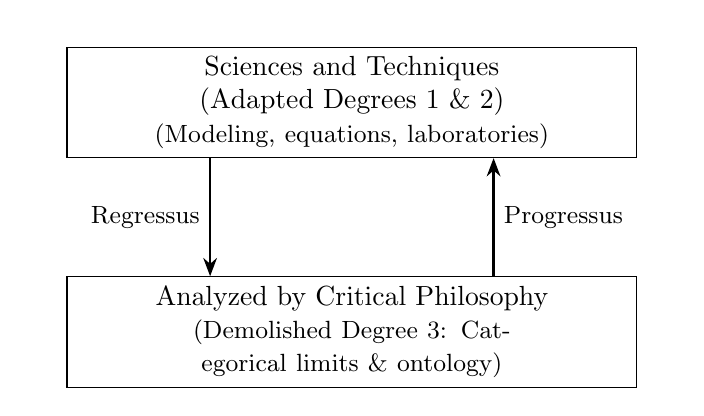
\begin{tikzpicture}[node distance=1.5cm, auto, >=Stealth]
\node (title2) [text width=8cm, align=center] {};
\node (box1) [below=0cm of title2, draw, rectangle, text width=7cm, align=center, minimum height=1cm] {Sciences and Techniques (Adapted Degrees 1 \& 2) \\ \small(Modeling, equations, laboratories)};
\node (box2) [below=1.5cm of box1, draw, rectangle, text width=7cm, align=center, minimum height=1cm] {Analyzed by Critical Philosophy \\ \small(Demolished Degree 3: Categorical limits \& ontology)};
% Loop Arrows (Regressus & Progressus)
\draw[->, thick, transform canvas={xshift=-1.8cm}] (box1) -- node[left] {\small Regressus} (box2);
\draw[->, thick, transform canvas={xshift=1.8cm}] (box2) -- node[right] {\small Progressus} (box1);
\end{tikzpicture}
\end{center} \vspace{-3ex}
\caption{ST-PM Reconfiguration: Critical-Materialist Loop}
\end{figure}



\subsection*{The PM reconfiguration of dialectics}

Within the framework of Gustavo Bueno's Philosophical Materialism (PM), the concept of the dialectical operative process represents a fundamental theoretical pillar that redefines traditional dialectical frameworks. In contrast to Hegelian idealism or Soviet dialectical materialism (\textit{Diamat})---which interpreted dialectics as abstract, metaphysical laws of either the mind or nature---Bueno anchors dialectics directly within the physical and corporeal operations of the gnoseological or operating subject. Under this approach, dialectics does not emerge from pure speculation; rather, it is constitutively operative and surgical. Logical and scientific operations originate through physical actions (such as separating, aligning, and measuring). When manipulating the terms of a material field, the researcher inevitably encounters objective contradictions that force the systemic reorganization of the framework.

This materialist interpretation of dialectics is structured across three core axes:

\begin{enumerate}
    \item {Dialectizing Analytical Logic:} Bueno rejects the formal separation between a strict analytical logic and an independent ``dialectical logic.'' Instead, he proposes to dialectize analytical logic, demonstrating how objective contradictions are implicitly embedded within formal logical operations and real-world material structures when distinct operative pathways interfere with one another.
    \item {Dialectics as Contradiction Resolution and Multilateralism:} PM retrieves the two most robust historical dimensions of the dialectical tradition. In its strong sense, it denotes the direct confrontation with objective contradictions and the explicit mechanisms through which systemic structures resolve internal incompatibilities to achieve stability. In its multilateral sense, it characterizes entities not as isolated nodes, but through the multiplicity of their interconnected and reciprocal relationships.
    \item {From Class Dialectics to State Dialectics:} Moving into the historical and political domains, Bueno critiques classical Marxist reductionism for focusing exclusively on class struggle. Instead, he highlights the concept of state dialectics, arguing that global historical and political dynamics are primarily governed by the conflict, scale of dominance, and mutual interference among empires and nations on the geopolitical stage.
\end{enumerate}

\subsubsection*{The dialectical circular structure in PM} \label{sec:pmregprog}
Bueno formally redefined the logical binomial to delimit the role of philosophy itself in relation to the positive sciences:
\begin{itemize}
	\item \textrm{Philosophical \textit{Regressus}:} the philosopher necessarily starts from the concepts and technical instruments provided by the positive sciences and mundane practices. The \textit{regressus} consists in dismantling, crushing, and deconstructing these particular scientific categories to ascend analytically toward the web of ontological \textrm{Ideas} that cross and structure them.
	\item \textrm{Philosophical \textit{Progressus}:} once the architecture of Ideas is systematized on the abstract level of the system, the philosopher is obliged to return critically to the starting point. He exercises the \textit{progressus} by returning to the original scientific categories and political or moral practices, but now equipped to reorder them, denounce their conceptual mythologies, and clarify their inner connections.
\end{itemize}

\subsubsection*{Relation to the Theory of Categorial Closure (TCC) and Synthetic Identity}
The most rigorous application of this circular scheme to Bueno's gnoseology is formalized in his \textrm{Theory of Categorial Closure (TCC)}, which describes the process by which a science becomes independent of philosophy and the scientist's psychology:
\begin{itemize}
	\item \textrm{Operative \textit{Regressus}:} in the development of scientific research, the operating subject (the researcher) physically intervenes upon the bodies of the field (terms). Through this material, surgical, and technological \textit{regressus}, the scientist segregates or neutralizes his own psychological subjectivity to distill purely objective relations among the terms of matter.
	\item \textrm{Synthetic Systematic Identity (SSI):} The fundamental core of any scientific truth occurs when the material chaining of operations gives birth to a confluence of terms that fit together perfectly in an objective, autonomous, and necessary way (e.g., the formulation of the periodic table or Kepler's laws). This structured objective truth is what Gustavo Bueno defines as a \textrm{Synthetic Systematic Identity (SSI)}.
	\item \textrm{Categorial Closure:} Upon reaching the SSI, the scientific field experiences a gnoseological ``closure.'' Subsequent scientific operations do not escape the boundaries of the field; rather, they reproduce circularly and internally within the category itself without requiring external theological or metaphysical principles.
	\item \textrm{Scientific \textit{Progressus}:} once the closure of the SSI is established, science deploys its \textit{progressus}: it deduces new theorems within the closed category, predicts new phenomena, and expands human technical and technological mastery over the physical world.
\end{itemize}



\subsubsection{The Concepts of Model and Modeling within PM} \label{sec:model_pm}

Gustavo Bueno and the framework of Philosophical Materialism (PM) systematically criticized the indiscriminate use of the ``word model'' to avoid falling into theoreticism or gnoseological formalism. In contrast to traditional positivism, which assumes that sciences advance by developing models of reality,'' PM isolates fundamental methodological risks within this approach:

\begin{enumerate}
\item {The Risk of Theoreticism and Fictionalism:} Reducing a science to a collection of models implies that scientific theories are merely mental constructs, useful maps, or convenient fictions designed for data-fitting. PM strongly argues that sciences do not build fictions; instead, they discover objective truths and synthetic identities through categorial closure. Scientific fields interact directly with empirical matter, not with abstract substitutes.
\item {The Risk of Formalism:} Formalism claims that abstract logical structures or mathematics represent the definitive model for any systematic knowledge. PM rejects this premise, stating that a discipline does not achieve scientific status by copying a formal mathematical template, but rather because it successfully closes its own material field via physical operations.
\item {The Representation Trap and Adequationism:} The word ``model'' carries the assumption of an external reality and an internal mental drawing that represents it. For PM, this fallback constitutes an unsustainable metaphysical dualism inherent to adequationism. PM circularism dismantles this dualism: the researcher does not stand outside looking in; the operator is embedded within reality, physically intervening through material tools and instruments to segregate the objective truth of the network.
\end{enumerate}


When the Theory of Categorial Closure utilizes the concept of a model, it classifies it strictly according to the theory of totalities into four distinct modalities:

\begin{itemize}
\item {Metric Model:} Rooted in quantitative relations and scaled physical measurements.
\item {Paradigmatic Model:} Operating as an archetypal reference or benchmark within the field.
\item {Prototypical Model:} Acting as the operational guide or normative design for a material construction.
\item {Canonical Model:} Defining the formal structural rule that modulates the interaction of interconnected parts.
\end{itemize}

However, the specific type of model analyzed in this study does not correspond to any of these four modalities. Instead, it aligns directly with the architectural paradigms documented in foundational systems modeling literature~\cite{Wellstead79}, which primarily focus on characterizing the temporal behavior of physical systems and are formally expressed through systems of differential equations.

Thankfully, within the Theory of Categorial Closure from Philosophical Materialism, this dynamic and temporal modeling approach finds its ultimate gnoseological justification through the broader concept of Synthetic Identity (``Identidad Sintética''). Rather than treating differential formulations as mere mathematical tools, the PM framework integrates the modeling of complex dynamic systems into a systematic circuit where truth is segregated through material and abstract operating courses. In the following section, this operational interaction between systems modeling and the Theory of Categorial Closure is thoroughly developed to establish the modeling foundations of the proposed power system architectures.


\subsubsection*{The Modeling Process in PM} \label{sec:modeling_process_pm}

Consequently, Philosophical Materialism avoids defining scientific activity as the mere fabrication of models. Instead, science achieves categorial closures that isolate material and objective truths, shifting away from the conception of theories as subjective representations of the physical world. Within this framework, a model does not represent a unidirectional path leading from reality to theory; instead, it constitutes a single phase within the closed loop of the modeling process. In other words, the modeling process operates as the explicit workflow through which the engineer embeds empirical matter into a formal structure to achieve, via experimental validation, a systematic synthetic identity that isolates the objective truth of a system.

\begin{figure}[h]
\begin{center}
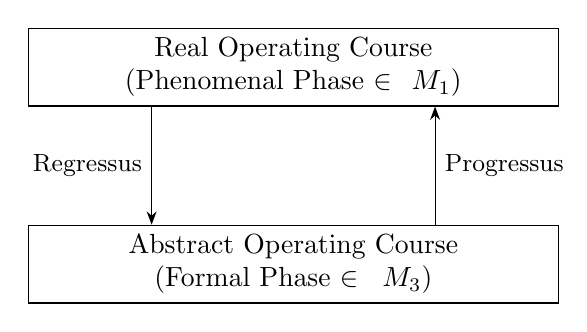
\begin{tikzpicture}[>=Stealth]
\node (box1) [draw, rectangle, text width=6.5cm, align=center]
{Real Operating Course \\
(Phenomenal Phase $\in M_1$)};
\node (box2) [below=1.5cm of box1, draw, rectangle, text width=6.5cm, align=center]
{Abstract Operating Course \\
(Formal Phase $\in M_3$)};
\draw[->, transform canvas={xshift=-1.8cm}] (box1) -- node[left] {\small Regressus} (box2);
\draw[->, transform canvas={xshift=1.8cm}] (box2) -- node[right] {\small Progressus} (box1);
\end{tikzpicture}
\end{center}\vspace{-3ex} \caption{The bidirectional Modeling Process within the ST-PM framework.} \label{fig:modeling}
\end{figure}

Adapting this intuitive engineering practice into the gnoseological framework of PM requires breaking the traditional realist illusion of adequationism—the naive assumption that an abstract mathematical model is a passive mental copy of a pre-structured external nature. To avoid this dualism, the model must be conceptualized during the active phase of the abstract operational course (Formal Structure) that converges with the real one, as illustrated in Figure~\ref{fig:modeling}:

\begin{itemize}
\item {Abstract Operating Course (Formal Phase in
$M_3$):} This course encompasses the formal operations executed by the researcher upon graphic signs, algebraic structures, and numerical code. The modeler manipulates terms, formulating systems of ordinary differential equations (ODEs) and applying numerical integration algorithms to generate a discrete time-series of values representing the temporal evolution of the system.

\item {Real Operating Course (Phenomenal Phase in
$M_1$)}: this course involves the hands-on and physical operations performed on the bodies being modeled. The engineer connects and manipulates hardware equipment and sensors to take measurements, and records the measurement data obtained from the instruments (such as oscilloscopes or smart meters).
\end{itemize}

The  Systematic Synthetic Identity emerges only when these operational courses
culminate in a very close convergence between them, showing a scientific truth is established; then the operating subject is neutralized.

Also, it's worth mentioning that in any modeling process, achieving this convergence is rarely an instantaneous event. Instead, it demands a recursive, trial-and-error optimization workflow. The modeler must execute successive iterations—adjusting parameters, recalibrating coefficients, and refining structural equations—to progressively fit the messy telemetry of the phenomenal course into the rigid geometric constraints of the abstract model.


In summary, what classical technical literature defines as the ``mathematical model'' of a physical process corresponds precisely to this formal structure, blueprint, or pattern within the abstract operating course, serving as the prescriptive mold into which empirical data must be operationally fitted to yield objective scientific truth.



\subsubsection{Astronomy example} \label{astro_example}

Johannes Kepler (1571–1630) was a German astronomer and mathematician of humble origins. Despite his family's financial instability and his own frail health, his brilliance enabled him to study theology at the University of Tübingen with the intention of being ordained as a Lutheran pastor. There, his mathematics and astronomy teacher, Michael Maestlin, introduced him to Copernicus's heliocentric theory—which was then considered contrary to Holy Scripture, as the latter supported Ptolemy's traditional geocentrism.

Before even completing his studies at Tübingen—at just twenty-two years of age—he secured a position as a mathematics teacher in Graz, Austria, in 1594, following the death of the previous incumbent. However, in 1600, he was soon expelled due to a decree issued by Archduke Ferdinand of Habsburg against Lutheran teachers, leaving him overnight without a home or a means of livelihood.

Kepler then traveled to Bohemia and presented himself at Tycho Brahe’s astronomical observatory, located on the outskirts of Prague. At first, Tycho—an extremely guarded aristocrat—took him in merely as a ``guest''; instead of granting him free access to his documents, he provided him with only small, isolated fragments of data. After two months of a difficult living arrangement marked by mutual distrust and arguments, Kepler finally reached an agreement with Tycho, subsequently moving his family to Prague and becoming his principal assistant.

Upon Brahe’s death in 1601, Kepler inherited his huge catalog of astronomical observations, which contained exhaustive notes on planetary positions. He spent nearly five years attempting to fit the observed positions of Mars into circular orbit models using geometric methods; he eventually succeeded in creating a model that worked almost perfectly, save for a discrepancy of 8 arcminutes at certain points along the trajectory (roughly one-quarter of the full moon's diameter).

Kepler placed blind faith in his mentor's precision, asserting that Tycho's data could not be wrong: ``If I had believed we could ignore those 8 minutes, I would have patched up my hypothesis accordingly. But since it was not permissible to ignore them, those 8 minutes alone have paved the way for reforming the whole of astronomy,'' he stated.

The process unfolded as follows:

1. Tycho Brahe’s data on Mars presented an astronomical nightmare because the planet's apparent motion across the sky traced very strange loops and curves. Kepler took up the challenge, convinced that planets must move in perfect circles combined with other, smaller circles (epicycles). He tried dozens of circular combinations and arrived at a model that missed Tycho’s recorded observations by a mere 8 arcminutes (a tiny fraction of a degree). Instead of ignoring this small discrepancy, Kepler placed absolute trust in the pinpoint accuracy of his mentor's data and concluded that the circular model was incorrect.

Upon realizing that the orbit of Mars was ``flattened'' at the sides, Kepler began testing other geometric shapes. He therefore turned to Apollonius's treatise ``Conics'' (written in the 3rd century BC), which examined the mathematical properties of parabolas, hyperbolas, and ellipses.

When he attempted to fit the observations of Mars into an ellipse, with the Sun positioned exactly at one of its foci (rather than at the center), the magic happened: all of Tycho Brahe's data fit perfectly. From this monumental mathematical effort, his First Law of Astrodynamics was born.


\subsubsection*{The Systematic Synthetic Identity}

This fundamental concept within the Theory of Categorical Closure arises when two distinct operating courses converge, thereby isolating the operating subject. In this instance, these are designated as course A and course B.

Operative course A consists of a table of pairs of ecliptic longitude ($\lambda$) and latitude  ($\beta$) values for a celestial body (Mars, in this case).
These data are derived from the manuscript notebooks titled ``Observationes planetarum'' \cite{brahe1596observationes}, in which Tycho and his assistants recorded observations made using the instruments available at the time—such as the quadrant and sextant—which predated the telescope and were constructed by Tycho himself.

Operational course B consists of drawing an ellipse on paper. Kepler had studied the properties of conic sections (ellipse, hyperbola, and parabola) in depth—drawing upon the works of Apollonius of Perga (200 BC) \cite{apollonius1566conicorum}—and knew how to draw them masterfully.


Then Kepler introduced a revolutionary operation: he took the pairs of numerical data ($\lambda, \beta$) from Mars's trajectory (course A) and projected them onto a sheet of paper, mapping them onto a graphical representation of the ellipse (course B).


\begin{figure}[htbp]
\centering
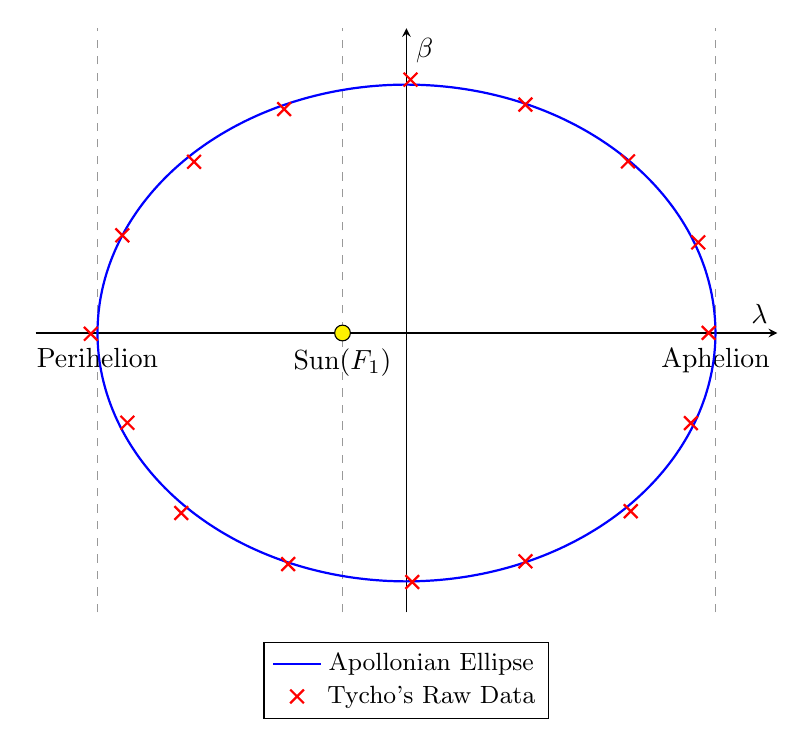
\begin{tikzpicture}
\begin{axis} [
    width=11cm,
    height=9cm,
    axis lines=center,
    xlabel={$\lambda$},
    ylabel={$\beta$},
    xmin=-6, xmax=6,
    ymin=-5.5, ymax=6,
    xtick={-5, -1.035, 0, 5},
    xticklabels={Perihelion, Sun($F_1$), 0, Aphelion},
    ytick=\empty,
    grid=major,
    grid style={dashed, gray!80},
    legend style={at={(0.5,-0.05)}, anchor=north, legend columns=1, font=\small},
    title={}
]

    % =========================================================================
    % 🎛️ CONTROL DE ERROR: Cambia este número para aumentar o disminuir el error.
    % 0.0  = Encaje perfecto (Identidad sintética absoluta).
    % 0.15 = Error sutil y realista.
    % 0.4  = Gran dispersión / Error grosero.
    % =========================================================================
    \newcommand{\ruido}{0.112}

    % 1. Elipse de Apolonio perfecta (El Molde ideal azul)
    \addplot[
        domain=0:360,
        samples=120,
        smooth,
        thick,
        blue
    ] ({5*cos(x)}, {4.89*sin(x)});
    \addlegendentry{Apollonian Ellipse}
	\fill[yellow, draw=black] (axis cs:-1.035, 0) circle (1mm);

    % 3. Puntos generados por función matemática con RUIDO ALEATORIO CONTROLADO
    % Se evalúan 16 puntos distribuidos uniformemente por la órbita (de 0 a 337.5 grados)
    \addplot[
        domain=0:337.5,
        samples=16,
        only marks,
        mark=x,
        mark size=3.5pt,
        thick,
        red
    ] ({5*cos(x) + \ruido*rand}, {4.89*sin(x) + \ruido*rand});
    \addlegendentry{Tycho's Raw Data}
\end{axis}
\end{tikzpicture}
\caption{Alignment between Thycho empirical observations and the ellipse model}
\label{fig:kepler_alignment}
\end{figure}


Both operating courses, coming from completely different contexts, fit together perfectly. The mathematical law of the ellipse, represented on the paper, and the actual physical trajectory of the planet, represented on the same paper and superimposed on the previous one, fit together with great precision. Figure \ref{fig:kepler_alignment} illustrates the process.

According to Philosophical Materialism, scientific truth is born from the comparison between two different operational courses that converge and fit together, resulting in a Systematic Synthetic Identity, in this case Kepler's First Law.


\subsubsection*{Regressus-Progressus omnipresence in Western philosophy}

The analyzed thread demonstrates a persistent isomorphism in the history of Western philosophy. The bi-directional circuit conceptualized by medieval scholasticism to bridge the gap between the sensible and the intelligible mutated in the 17th century into the methodological framework of the physical-mathematical sciences. Finally, in contemporary times, Gustavo Bueno's Materialism Philosophy (PM) demystified these processes by showing that rigorous knowledge, whether scientific or philosophical, never stops at an inert contemplative abstraction. Instead, it always requires a recursive return to material operations and the empirical field where the objective identities of reality are forged.

The following table condenses the historical and gnoseological evolution of the logical double transit and the treatment of abstraction across the four analyzed modeling approaches:

% =========================================================================
% PARTE 3: MATRIZ COMPARATIVA GENERAL Y CONCLUSIÓN
% =========================================================================
\begin{table}[h!]
    \centering
    \caption{Gnoseological isomorphism from Thomistic Abstraction to the Theory of Categorial Closure.}
    \label{tab:complete_gnoseological_evolution}
    \vspace{0.3cm}
    {\footnotesize
    % Definimos una columna tipo X que justifica a la izquierda con buen manejo de guiones
    \newcolumntype{Y}{>{\RaggedRight\arraybackslash}X}
    % Asignamos un ancho fijo holgado a la primera columna para evitar saltos feos
    \begin{tabularx}{\textwidth}{p{3.4cm}YYY}
    \toprule
    \textbf{Philosophical Model} & Starting Point & Regressus & Progressus \\
    \midrule
    Thomas \newline Aquinas (ST) & The \textit{phantasm} (individual sensible image). & Formal abstraction (\textit{abstractio}) of essences from matter. & \textit{Conversio ad phantasmata}: predication of the universal onto the concrete entity. \\
    \addlinespace
    School of \newline Padua & Observable empirical and qualitative effect. & \textit{Resolutio} (\textit{demonstratio quia}): induction from effect to cause. & \textit{Compositio} (\textit{demonstratio propter quid}): deduction of the effect from the cause. \\
    \addlinespace
    Modern \newline Science & Physical phenomenon quantitatively measurable. & Analysis / Resolution: quantitative reduction and mathematical modeling. & Synthesis / Composition: numerical deduction and controlled experiment. \\
    \addlinespace
    Philosophical \newline Materialism (PM) & Categorial concepts of sciences and techniques. & Analytical dismantling (\textit{trituración}) toward ontological Ideas. & Critical deployment of the system of Ideas upon practical categories. \\
    \addlinespace
    Categorial Closure \newline Theory (TCC) & Material terms of the scientific disciplines. & Operative \textit{regressus}: neutralization of the physical/gnoseological subject. & Scientific \textit{progressus}: synthetic construction and technology after \textit{SSI}. \\
    \bottomrule
    \end{tabularx}}
\end{table}


\subsubsection{Pragmatic utility of the developed modeling approach} \label{sec:pragmatic_utility}

A legitimate question may arise from a strictly practical engineering perspective after evaluating this conceptual background: why should a researcher encumber power systems modeling with rigorous philosophical epistemology when numerical algorithms can be coded and computed without it? The answer does not reside in abstract contemplation, but in providing a foundational quality control framework for the modeling process itself, particularly when dealing with complex, decentralized, and renewable-dominated smart grids. Without a structured gnoseological scheme, the systems engineer inevitably falls into two operational traps: \textit{theoreticism} (confusing the clean trajectories on a computer screen with the messy reality of the physical asset) or \textit{descriptionism} (accumulating vast streams of sensor telemetry from smart meters without a formal structure to isolate objective relations).

The recursive \textit{Regressus-Progressus} circuit yields four immediate pragmatic advantages in modern engineering design:
\begin{enumerate}
    \item {Streamlined code and hardware implementation:} By utilizing an explicit epistemological framework, the modeler maps out exactly what the model represents and where its mathematical boundaries lie before implementation. This conceptual pre-structuring severely reduces developmental overhead, making the translation of classified abstract objects into high-performance source code straightforward. Furthermore, it establishes a rigorous operational blueprint to synthesize novel hardware architectures and physical components based on verified structural invariants.
    \item {Surgical parameter simplification:} It provides a rigorous criterion to determine which secondary physical variables can be deliberately neutralized (e.g., minor thermal drifts or structural contingencies) to ensure mathematical tractability without breaking the material truth of the validation loop.
    \item {Systemic fault diagnosis:} When a simulation model fails to match laboratory behavior, this framework prevents blind trial-and-error parameter tuning. The modeler can systematically isolate whether the breakdown occurred during data acquisition (\textit{Phenomenal Praxis}), structural abstraction (\textit{Regressus}), or subject-disconnection within the return path (\textit{Progressus}).
    \item {Cyber-Physical anomaly detection:} In first-order Digital Twins governed by the $(P, \eta)$ syntax, this approach establishes that a model is not a passive representation of the grid, but an autonomous gnoseological closure. Consequently, if a cyber-attack injects false telemetry that satisfies statistical expectations but violates the core structural invariants of the categorical closure, the system immediately flags the anomaly.
\end{enumerate}


%{\color{red} Ultimately, developing models without a critical epistemology is akin to piloting an aircraft by instinct. While this may suffice for simple configurations, advanced multi-agent systems and complex electrical grids require precise structural analysis to guide mathematical modeling~\cite{lu2025enhanced}---thereby transforming modeling engineering from a mere exercise in statistical data fitting into a powerful operational tool.
%
%}
Ultimately, developing models without a clear conceptual framework reduces engineering to blind guesswork. While a simple trial-and-error approach may suffice for basic configurations, advanced multi-agent systems and complex electrical grids require a clear structural understanding to guide mathematical modeling---thereby transforming engineering from a mere exercise in statistical data fitting into a powerful operational tool.


\subsection{Other Philosophies} \label{sec:other_philosophies}

While this review article adopts the Theory of Categorial Closure from Philosophical Materialism as its primary epistemological benchmark, a systematic evaluation of other modern and contemporary philosophical frameworks reveals that they provide valuable, albeit fragmented, tools for abstract modeling and systems theory. Rather than dismissing these historical traditions, their core contributions toward structural isomorphism, empirical validation, and causality must be critically examined to determine their operational limits in engineering praxis.


\begin{enumerate}
    \item {The rationalist contribution and Theoreticism:} Modern rationalism (from René Descartes to Gottfried Wilhelm Leibniz) established the foundational confidence in the capacity of abstract, mathematical structures ($M_3$) to capture universal laws of nature. In systems modeling, this tradition highlights the power of formal deduction and analytical tractability. However, its gnoseological boundary resides in \textit{theoreticism}: it tends to treat physical systems as pure geometry, overlooking the fact that empirical matter ($M_1$) imposes non-linear, stochastic constraints (such as thermal drifts or chemical degradation) that formal mathematical logic alone cannot predict.

    \item {The empirist contribution and Descriptionism:} Conversely, the empiricist tradition and subsequent logical positivism (from David Hume to the early 20th-century philosophy of science) provided a necessary anchor in raw data acquisition, sensory telemetry, and controlled laboratory experimentation. This operational demand directly maps onto modern system identification methods. Its main epistemological risk, however, is \textit{descriptionism} or \textit{fictionalism}. By reducing causality to a mere spatiotemporal regularity or statistical conjunction of events, it downgrades mathematical models to convenient data-fitting tools or cognitive fictions, stripping them of any claim to objective material truth.

    \item {General Systems Theory and Functionalism:} In the mid-20th century, Ludwig von Bertalanffy's General Systems Theory \cite{vonbertalanffy1968general} and Norbert Wiener's Cybernetics introduced a major milestone by identifying the concept of \textit{structural isomorphism}---the realization that identical differential equations or state-space matrices govern heterogeneous physical domains (e.g., matching mechanical mass-spring dynamics with electrical RLC circuits). GST shifted the focus from isolated components to interconnected networks governed by feedback loops. Despite this technical utility, GST often falls into an incomplete \textit{functionalism} or ``black-box'' approach. It effectively maps inputs and outputs but leaves the gnoseological boundary between subjective representation and material objectivity unresolved.

    \item {Critical Realism and Generative Causality:} As a contemporary alternative, Roy Bhaskar's Critical Realism \cite{bhaskar1975realist} successfully salvages efficient causality and ontological depth for systems engineering. CR establishes a stratified ontology divided into three distinct layers: the \textit{empirical} (sensor telemetry and direct observations), the \textit{actual} (the real-time events and power flows occurring within the grid), and the \textit{real} (the underlying generative mechanisms and physical structures possessing causal powers). Under this framework, abstract modeling operates via \textit{retroduction}—abstracting from empirical observations to map the invariant generative structures of the real world. Nevertheless, CR frequently remains overly speculative and detached from algorithmic implementation.

    \item {Scientific Entity Realism (the new Experimentalism):} Formulated by Ian Hacking in the late 20th century \cite{hacking1983representing}, Entity Realism (\textit{experimental realism}) introduces an architectural paradigm that shares profound structural convergences with Gustavo Bueno's Philosophical Materialism~\cite{madrid2006nuevo} \cite{madrid2006nuevo}. Hacking executed a radical shift from traditional theory-centered realism toward experimental practice itself, defining scientific objectivity not through linguistic representation (\textit{representing}), but through material intervention and physical manipulation (\textit{intervening})~\cite{hacking1982experimentation}. Under this scope, theoretical entities (such as electrons) are validated as objective realities if and only if they can be routinely manipulated as tools to create causal effects in independent operational domains—crystallized in Hacking's aphorism: ``if you can spray them, then they are real''~\cite{hacking1984experimentation}. This perspective directly aligns with the $\beta$-operative phase of the Theory of Categorial Closure, where the researcher's hands and instruments physically transform fields to isolate structural invariants. Nevertheless, entity realism exhibits a clear operational limit: by focusing exclusively on the physical manipulation of hardware, it remains skeptical of high-level mathematical simulations and abstract software platforms, failing to fully justify the validity of system-wide digital twins.
\end{enumerate}



\subsubsection*{Similarity between PM New Experimentalism}

While both New Experimentalism and Philosophical Materialism converge on the idea that science is grounded in bodily and instrumental manipulation within the laboratory, they fundamentally diverge regarding the ultimate status of the human actor once scientific truth is achieved. This distinction centers on Gustavo Bueno's concept of the {``segregation of the subject''} (\textit{segregación del sujeto}).

Within the Anglo-American tradition of New Experimentalism (e.g., Ian Hacking), truth and reality remain tethered to the scientist's intervention.
\begin{itemize}
    \item {Pragmatic Realism:} reality is validated through successful manipulation (``if you can spray them, they are real'').
    \item {The human footprint:} The scientist's operations, experimental designs, and physical actions do not disappear from the epistemic equation. Scientific truth is justified precisely because human agents can predictably alter the world using laboratory tools.
\end{itemize}

Conversely, for Gustavo Bueno's \textit{Theory of the Categorical Closure} (\textit{Teoría del Cierre Categorial}), physical manipulation is done only while the operating courses are running but cease when they converge and then a scientific truth {theorem} is reached.

Thus, this short critical review of alternative philosophies demonstrates that while each framework captures a specific phase of the modeling process, they often fail to achieve a fully circular integration. Philosophical Materialism bridges these partial insights: it honors the formal rigor of rationalism and the empirical demand of empiricism, but unifies them through the physical, $\beta$-operative praxis of the researcher. The abstract model is thus validated neither as a pure mathematical ideal nor as a convenient statistical fiction, but as an objective structural node that effectively achieves categorial closure within the material dynamics of the physical environment.



\section{Case studies using the ST-PM framework}
To illustrate the scalability and universal validity of the ST-PM philosophical-technical framework, four progressive examples are presented. These range from fundamental multi-domain physics to a complex chemical process extracted from recent industrial literature.

\subsection{A mechanical mass-spring-damper system}
Consider a classical mechanical system governed by a mass $m$, a spring constant $k$, a viscous damping coefficient $b$, and an external applied force $f(t)$.
\begin{itemize}
\item \textrm{Phase 1 (Sensible Matter):} The physical hardware consists of a specific steel block, a physical coiled spring, and a hydraulic cylinder filled with oil ($M_1$). The first degree of abstraction discards individual impurities, the temperature of the oil, or the color of the metal to retain only the generalized parameters ($m, k, b$).
\item \textrm{Phase 2 (Intelligible Matter):} The system undergoes a transformation into a device-independent abstraction ($M_3$). Newton's second law translates the physical body into a second-order ordinary differential equation (ODE):
\begin{equation}
m\ddot{x}(t) + b\dot{x}(t) + kx(t) = f(t)
\end{equation}
At this stage, the mechanical nature fades; the system is structurally identical to an electrical RLC circuit. It is pure relation and extension.
\item \textrm{Phase 3 (Systematic Synthetic Identity):} The model achieves its truth within the closed category of Classical Mechanics. The systematic synthetic identity is established when the numerical solution of the ODE ($M_3$ - Formal Course) matches the data collected by position and force sensors ($M_1$ - Empirical Course) during laboratory testing ($M_2$).
\end{itemize}

\subsection{Stoichiometric chemical process ($2\text{H}_2 + \text{O}_2 \rightarrow 2\text{H}_2\text{O}$)}
Let us analyze the fundamental synthesis reaction of water from molecular hydrogen and oxygen.
\begin{itemize}
\item \textrm{Phase 1 (Sensible Matter):} The empirical reality involves gas cylinders, pressures, temperatures, and the violent, exothermic nature of the molecular collision ($M_1$). Abstraction segregates the individual container geometries to focus on the sensible general properties of the reactants.
\item \textrm{Phase 2 (Intelligible Matter):} The reaction is stripped of its physical violence and mapped into an abstract, device-independent relational structure via stoichiometry and chemical kinetics:
\begin{equation}
\frac{d[\text{H}_2\text{O}]}{dt} = k(T)[\text{H}_2]^2[\text{O}_2]
\end{equation}
The chemical reaction is now represented as an algebraic-differential graph in $M_3$.
\item \textrm{Phase 3 (Systematic Synthetic Identity):} The model does not possess its own closure; it embeds itself within the core of Chemical Thermodynamics. The identity is synthesized when the computer-simulated reaction rates and yield curves ($M_3$) perfectly match the gas chromatography measurements ($M_1$) under varying initial concentrations.
\end{itemize}

\subsection{The electrical voltage divider}
Consider a DC voltage source $V$ connected to a voltage divider consisting of two resistors, $R_1$ and $R_2$, where the useful power is defined in terms of generator power and efficiency ($\eta$).
\begin{itemize}
\item \textrm{Phase 1 (Sensible Matter):} The hardware comprises copper wires, breadboards, and carbon-film resistors that dissipate heat ($M_1$). Abstraction discards the physical routing and temperature-induced resistance drifts to isolate the nominal Ohm values.
\text{Phase 2 (Intelligible Matter):} Using Kirchhoff's laws, the physical circuit is converted into an abstract relational network ($M_3$) governed by generalized power-flow formulations:
\begin{equation}
P_{\text{util}} = P_{\text{gen}} \cdot \eta, \quad \text{where } \eta = \frac{R_2}{R_1 + R_2}
\end{equation}
The circuit becomes a pure mathematical optimization problem, independent of whether the resistors are made of ceramic or semiconductor materials.
\item \textrm{Phase 3 (Systematic Synthetic Identity):} The closure is provided by Electrodynamics. The abstract equations are validated when the measured voltages and thermal efficiency metrics ($M_1$) match the predicted mathematical curves ($M_3$) during actual hardware operation ($M_2$).
\end{itemize}

\subsection{Catalytic cracking of fusel oil for light olefins production}
Our final case study examines a highly complex industrial process found in recent literature: the fluid catalytic cracking (FCC) of fusel oil over an HZSM-5 catalyst to produce light olefins.
\begin{itemize}
\item \textrm{Phase 1 (Sensible Matter):} The physical setup involves a fixed-bed reactor, complex mixtures of biowaste (fusel oil containing ethanol, propanol, and heavy alcohols), and a porous crystalline catalyst operating at high temperatures ($M_1$).
\item \textrm{Phase 2 (Intelligible Matter):} To elevate this industrial process to control engineering, it must be rewritten using the ST-PM framework. The chaotic mixture of the feed must be simplified into a ``lumped'' kinetic model (e.g., 3-lump or 4-lump models), and the reactor topology must be mapped into multi-phase mass and energy balance ODEs ($M_3$):
\begin{equation}
\rho u \frac{\partial Y_i}{\partial z} = \sum_{j} \nu_{ij} r_j
\end{equation}
Through this device-independent mathematical graph, the physical fixed-bed is converted into an abstract system of state variables.
\item \textrm{Phase 3 (Systematic Synthetic Identity):} In the original experimental paper, the authors limited their work to Phase 1 and empirical parameter fitting, lacking an abstract control-oriented framework. To achieve a true ST-PM abstraction, a \textit{regressus} is mandatory. The mathematical lumped kinetic model ($M_3$) must run in a real-time simulator. The synthetic identity is achieved when the simulated olefin yields and catalyst deactivation curves over time ($M_3$) precisely predict the experimental gas chromatography time-series ($M_1$) across different space velocities. This encasement within the category of Chemical Engineering turns a purely descriptive laboratory experiment into an operational, scalable model for process control.
\end{itemize}



\section{Application to Renewable Energy Systems}



In what follows, the aforementioned philosophical frameworks—integrating Scholastic abstraction, the dual transit of \(\textit{Regressus} and \textit{Progressus},\) and Philosophical Materialism (PM)—shall be applied to the context of modeling renewable energy systems.

As established, abstraction in the Thomistic sense operates sequentially. First, through physical abstraction, which isolates and selects only the objects of interest from the empirical field; second, through mathematical abstraction, which performs measurements upon a real, physical object $O$ (in $M_1$) to extract quantitative data and arrange it into a structured, formal framework or model (in $M_3$). Finally, this model of $O$ is systematically projected back onto reality to verify its fit, completing the circular transit of \textit{regressus} and \textit{progressus}. Consequently, our application begins by addressing the initial phase of this methodology: physical abstraction.


To operationalize this first phase of physical abstraction, a decisive simplifying assumption is made: the power systems under analysis operate entirely in direct current (DC). This drastic reduction of the physical field is highly accurate and structurally justified for a wide array of modern architectures, such as microgrids composed of photovoltaic generation, battery energy storage systems, and wind turbines coupled with DC links.

Evidently, this simplifying decision does not capture the full, multi-faceted complexity of contemporary large-scale power grids. However, this constitutes a calculated trade-off; by filtering out the dynamics of alternating current (AC) factors—such as frequency fluctuations, reactive power, and phase angles—computational overhead is drastically reduced. This analytical reductionism isolates the core energetic behavior of the microgrid, providing a highly scalable and mathematically tractable baseline for advanced operation and control. ``

A further step in physical abstraction consists of selecting a fundamentally simple circuit to serve as the elementary building block: the voltage divider. By employing this basic element through an operational synthesis, diverse components across the entire power grid can be systematically modeled. For the scope of this initial framework, the analysis is restricted to steady-state operations, thereby assuming a static behavior that remains independent of time \(t\)


This process of physical abstraction—corresponding to the first Thomistic degree—consists of selecting a fundamentally simple circuit to serve as the elementary building block: the voltage divider. Immediately following this choice, the second degree of abstraction (mathematical abstraction) is applied to extract its formal DC model. This mathematical structure is first developed in terms of classical circuit variables, such as voltages and resistances (\(V, R_1, R_2\). Through a subsequent algebraic transformation, these relations are translated into a power-oriented framework characterized by power variables and efficiency indices (\(P_1, P_2, \eta\).


By employing this basic mathematical element through an operational synthesis, diverse components across the entire power grid can be systematically modeled. For the scope of this initial framework, the analysis is restricted to steady-state operations, thereby assuming a static behavior that is independent of time (\(t\).

Finally, the modeling phase proper is reached, driven by the operational loops of \textit{regressus} and \textit{progressus}:
the dynamic modeling of direct current (DC) distribution networks. By applying the concept of Synthetic Identity from Philosophical Materialism (PM)—which structurally implicates these bidirectional transits—a novel, objective component is formulated in $M_3$
\textit{Hybrid Bus (Hbus)}  $M_3$ termed the \textit{Hybrid Bus (Hbus)}. This component enables the modeling of radial power networks using a System Dynamics framework. Notably, restricting the scope to radial topologies represents an additional step in physical abstraction (the first Thomistic degree), aligning the analysis with the structural configurations typically featured in foundational Power Systems literature.


In short, by leveraging Gustavo Bueno’s Theory of Categorial Closure (TCC), a gnoseological closure is operated, establishing a new scientific category. Within this closed domain, traditional circuit-level variables—such as node voltages ($V$), branch currents ($I$), and line resistances ($R$)—completely disappear or are neutralized. They are systematically replaced by a pure power-oriented syntax governed exclusively by power variables and efficiency metrics ($P, \eta$).



\subsection{Voltage Divider circuit}

Adopting a bottom-up approach, our modeling of electrical networks initiates
from the most elementary non-trivial circuit, namely the
voltage divider (VD). A VD comprises a voltage source $V$ impressed upon a series connection of two resistive elements, $R_1$ and $R_2$. This configuration is denoted by the tuple $(V; R_1, R_2)$. The device operates by partitioning the total
applied voltage $V$ into constituent voltage drops $v_{12}$ and $v_{20}$,
satisfying the relation $V = v_{12} + v_{20} = v_{12} + v_{2}$ since by convention $v_0=0$.

We define the physical parameter space of a voltage divider as the set $S$ of ordered pairs of non-negative resistances, excluding the origin to avoid mathematical indeterminacies:
\[
S = \mathbb{R}_+^2 = \{ (R_1, R_2) \in \mathbb{R}^2 \mid R_1 \ge 0, \, R_2 \ge 0 \} \setminus \{(0,0)\}
\]
A parameterized voltage divider circuit is determined by the triplet $(V, R_1, R_2)$, where $V \in \mathbb{R}^+$ represents the magnitude of the voltage source. By Ohm's law, the net current of the circuit satisfies:
\[ I = \frac{V}{R_1 + R_2} \]
as Figure \ref{fig:circuitvR1R2sch} shows, with $v=V$ and $i=I$.
\begin{figure}[h!]
	\centering
	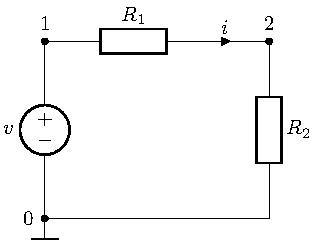
\includegraphics[width=0.36\linewidth]{figs_tikz/circuitVR1R2sch}
	\caption{Voltage Divider}
	\label{fig:circuitvR1R2sch}
\end{figure}

We will now introduce the voltage attenuation operator $\Gamma: S \to [0, 1]$,
which maps each pair of components to its respective scalar transfer factors or
attenuation ratios:
\[ \gamma_1 = \frac{R_1}{R_1 + R_2}, \quad \gamma_2 = \frac{R_2}{R_1 + R_2} \]
The partial voltages of the circuit satisfy the direct algebraic coupling
$v_{12} = \gamma_1 V$ and $v_{20} = \gamma_2 V$. Since $\gamma_1 + \gamma_2 = 1$, the device behavior is entirely characterized by a single ratio $\gamma = \gamma_2$
\begin{equation}
\gamma = \frac{R_1}{R_1 + R_2}
\label{eq:atenuacion}
\end{equation}


To formalize this behavior,  a binary relation $\sim$ is established on the set $S$, defined as:
\[ (R_1, R_2) \sim (R'_1, R'_2) \iff \Gamma(R_1, R_2) = \Gamma(R'_1, R'_2) \iff \gamma = \gamma' \]
This relation constitutes an equivalence relation because evidently it fulfills the reflexive, symmetrical and transitive properties.
It groups all resistor pairs $(R_1, R_2)$ that yield
exactly the same attenuation factor $\gamma$ within the voltage divider.
From a physical standpoint, this means that all circuits belonging to the same
equivalence class scale down the input voltage in precisely the same proportion, regardless of the absolute ohmic values of the individual resistors.

Regarding the quotient space, each equivalence class $[(R_1, R_2)]$ is uniquely
identified by its attenuation factor $\gamma$. The quotient set $S/\!\!\sim$,
which gathers all possible equivalence classes, is in direct bijection with the
closed real interval of the attenuation factors:
\[ S/\sim \; \cong [0, 1] \]

Consequently, the attenuation of a voltage divider is entirely characterized by
a single real number $\gamma \in [0, 1]$, instead of requiring an infinite
number of possible resistor pairs.


To understand the geometric shape of these equivalence classes, the condition derived from the operator is developed:
\[
\frac{R_2}{R_1 + R_2} = \gamma \implies R_2 = \gamma R_1 + \gamma R_2 \implies R_2(1 - \gamma) = \gamma R_1
\]
By solving for $R_2$ as a function of $R_1$ for a fixed value of $\gamma$
(where $0 \leq \gamma < 1$), the linear equation
\[
R_2 = \left( \frac{\gamma}{1 - \gamma} \right) R_1
\]
is obtained. This expression represents a straight line passing through the origin in the
$\mathbb{R}_+^2$ plane. Since resistances must be non-negative, only the first quadrant is considered. Therefore, each equivalence class defines a ray or half-line
emanating from the origin $(0,0)$—with the origin itself excluded to prevent the
physical indeterminacy $0/0$—having a positive slope equal to $m = \frac{\gamma}{1 - \gamma}$.

This geometric interpretation yields three specific boundary cases:
\begin{itemize}
	\item If $\gamma = 0$ (implying $R_2 = 0$), the equivalence class corresponds to the horizontal axis ($R_1 > 0$).
	\item If $\gamma = 1$ (implying $R_1 = 0$), the equation simplifies to the vertical axis ($R_2 > 0$).
	\item If $\gamma = 0.5$ (implying $R_1 = R_2$), the equivalence class lies precisely on the bisector of the first quadrant ($R_2 = R_1$).
\end{itemize}

These boundary conditions highlight how the topology of the equivalence classes
projects specific behaviors at the limits of the design space. Specifically,
when $\gamma = 0$ ($R_2 = 0$), the equivalence class collapses onto the open
horizontal axis $R_1 > 0$. Conversely, when $\gamma = 1$ ($R_1 = 0$), it
collapses onto the open vertical axis $R_2 > 0$. Finally, when $\gamma = 0.5$
($R_1 = R_2$), the class strictly coincides with the bisector of the first quadrant.

\subsubsection*{Power in VD}

We assume resistance $R_2$ acts as the circuit load where useful power $P_u$ is utilized, i.e. $P_u = P_2 = R_2 I^2$, and that resistance $R_1$ represents the losses dissipated to the environment. The relationship between the useful power $P_u$ and the total power $P$ injected by the generator is the energy efficiency:
\[
 \eta = \frac{P_u}{P}
\]

To express these ideas formally, an energy efficiency operator
$\mathcal{H}: S \to [0, 1]$, is defined, by the ratio between the useful power and
the total input power $P = (R_1 + R_2)I^2$. This definition
reveals a direct algebraic duality, as the efficiency operator
\[ \mathcal{H}(R_1, R_2) = \frac{P_u}{P} = \frac{R_2 I^2}{(R_1 + R_2)I^2} = \frac{R_2}{R_1 + R_2} = \gamma \]
is identical to
the voltage attenuation operator (Equation \ref{eq:atenuacion}). Consequently, the previously defined equivalence relation can be reformulated from an energetic viewpoint, where two circuit configurations belong to the same
equivalence class if and only if they yield the exact same efficiency,
that is, $(R_1, R_2) \sim (R'_1, R'_2) \iff \eta = \eta'$.


\subsubsection*{Ratio of power (analogous to efficiency)}

In a resistive network, one doesn't usually speak of ``efficiency'' in the conventional sense (as in real machines or sources), since all the power injected by the generators is dissipated in the resistors. However, it is possible to define a useful power ratio if you consider that only a portion of the total power dissipated (for example, in a specific load $R_k$) is ``useful.''

\begin{equation}
\eta_k = \frac{P_{dk}}{P_{gj}} =
\frac{\text{power dissipated in}\, R_k}{\text{power injected by}\, V_j}
\label{eq:resistive_network}
\end{equation}

This value represents \text{the power of a generator is disrupted by a specific resistance} and it is always less than 1.

It is useful in power distribution analysis or when you want to maximize the power delivered to a specific load (as in the maximum power transfer theorem \cite{alexander2021fundamentals}).

It is not an ``efficiency'' in the thermodynamic sense, but a power distribution index.

This calculation can be performed after applying the mesh method, obtaining the currents in each element, calculating them
\[
P_{dk} = R_k I_k^2, \quad P_{gi} = V_i I_i
\]
and substituting them (\ref{eq:resistive_network}). In complex circuit configurations, this calculation is straightforwardly performed after applying mesh or nodal analysis to determine the branch currents, yielding:
\[
P_{dk} = R_k I_k^2, \quad P_{gj} = V_j I_j
\]
and subsequently forming the required quotient.




\subsection{Bus modeling in SD}

The dynamic behavior of System Dynamics (SD), based on finite difference equations, was described in Forrester (1961), p. 76. SD has two basic elements: the first, called Stock, represents inventory or storage variables, and the second, called Flow, represents flow variables. The equation that relates a stock $s$ to a net incoming flow $f$ is:

\begin{equation}
	f(k) = f(j) + \Delta t(s(k) - s(j))
	\label{eq:3}
\end{equation}
where $j < k$ are time points, $\Delta t$ is a time increment, and $f(t)$ and $s(t)$ are the flow and stock values at time $t$, respectively.

It is important to note that the net inflow is the sum of all inflows minus all outflows.

If the net inflow is equal at times $j$ and $k$, that is, $f(k) = f(j)$, then, according to equation \ref{eq:3}, $f(k) - f(j) = 0$ and
\begin{equation}
	s(k) = s(j)
	\label{eq:4}
\end{equation}
That is, the stock value remains constant. If, in addition, $s(j) = 0$, then the following holds true:
\begin{equation}
	s(k) = s(j) = 0
	\label{eq:5}
\end{equation}
so the stock value remains equal to zero. This can be related to the flow continuity equation \cite{Euler1757}, making an SD stock correspond to an electrical node, as detailed below.

The methodological divergence introduced in this work represents a paradigm shift in system modeling. While System Dynamics (SD) has been traditionally deployed as a \textit{top-down}, macroscopically oriented tool for policy analysis, infrastructure planning, and long-term energy balancing \cite{pr13092969, sys12040109}, this paper operates a radical \textit{bottom-up}, device-level synthesis. By tracking the immanent circuit laws (Kirchhoff's and Ohm's relations) and formalizing the instantaneous node closure via a proportional feedback loop within the Hybrid Bus (\textit{Hbus}) structure, a macro-level systems language is adapted to govern micro-level transient dynamics.  This framework bridges the gap between hardware-level hyperrealism and abstract multi-variable scaling without losing physical tractability at the boundaries.


\subsection{Modeling Power Systems in SD}

A Power System (PS) is an interconnected network of electrical components designed to generate, transmit, distribute, and utilize electrical energy efficiently and safely. The most common example is the large-scale grid that supplies electricity to homes and industries  \cite{Glover2012}. Modern power systems are often called Smart Grids and have evolved from the old electricity grid to the modern power systems, incorporating new technologies and equipment such as Renewable Energy Sources (RES), Energy Storage Systems (ESS), Inverter-Based Resources (IBRs), and more.

\subsubsection{Single-line diagrams} \label{sec:sld}

A schematic ubiquitously found in textbooks \cite{Glover2012}, technical reports, and engineering studies is the Single-Line Diagram (SLD). At its core, an SLD is a simplified notation used to map out critical components—such as generators, transformers, buses, and circuit breakers—along a single line.

These diagrams preserve the circuit topology and use a small segment of thick line called a \textit{bus} or \textit{bar} instead of a single point to represent each node. Their name and shape allude to those of their namesake components, such as a solid copper bar, in power plants, substations, and other power distribution centers in the electrical grid.

These diagrams are used to represent power flows ($p$) and efficiencies $(\eta)$ instead of the standard voltage and current variables $(v,i)$ and components ($R$) in circuits.

While historically designed for traditional three-phase AC networks, modern SLDs are also widely utilized to represent DC systems, including solar farms and battery storage facilities.

As an example, the SLD diagram of the circuit in Figure \ref{fig:circuitvR1R2sch} is shown in Figure \ref{fig:sldvr1r2l}, where nodes 1 and 2 are now labeled Bus1 and Bus2, respectively. The variables shown are no longer voltages or currents but only power $P$ and the efficiency parameter $\eta$. We can see that this diagram preserves the topology of the electrical circuit.

\begin{figure}[h!]
	\centering
	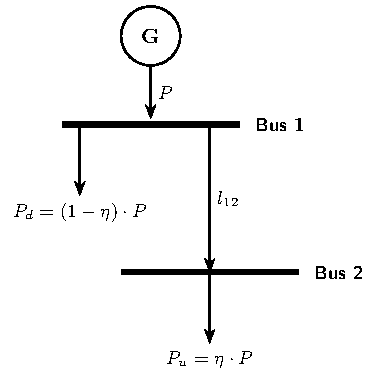
\includegraphics[width=0.4\linewidth]{figs_tikz/sldVr1r2lu}
	\caption{Voltage Divider SLD graph}
	\label{fig:sldvr1r2l}
\end{figure}

The following table shows the correspondence between the elements of both diagrams.

\begin{center}
	\begin{tabular}{c|c}
		Circuit &  SDL diagram\\ \hline
		Node 1 &  Bus 1 \\
		Node 2 &  Bus 2 \\
		Generator V &  Generator G \\
		Corriente i & Power P \\
		Components $R_1, R_2$  &  Efficiency $\eta$
	\end{tabular}
\end{center}

Line $l_{12}$ physically represents the electrical conductor that electrically connects the two buses and corresponds to the component $R_2$ of the circuit, where the dissipated power $P_d$ is released into the environment—that is, wasted.

\begin{figure}[h]
	\centering
	\begin{tabular}{ccc}
		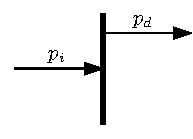
\includegraphics[height=0.13\linewidth]{figs_tikz/sl_busd} & \hspace{12ex} &
		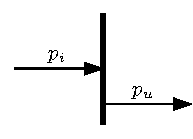
\includegraphics[height=0.13\linewidth]{figs_tikz/sl_busl}\\
		Bus $ 1 $ & & Bus $ 2 $
	\end{tabular}
	\caption{The two VD Buses}
	\label{fig:sl_busdl}
\end{figure}

As Figure \ref{fig:sl_busdl} shows, the buses from the SDL diagram shown in Figure \ref{fig:sldvr1r2l} have been depicted separately
(by removing the connection line $l_{12}$ that linked them), where $p_i$ denotes the incoming power flow. Clearly, $ p_d < p_i $, $ p_u < p_i $, and $ p_d + p_u = p_i $.

Looking at  Figure \ref{fig:sl_busdl}, and noting that both buses share the same incoming power $p_i$, one might think to combine them into a single composite bus with an incoming power $p_i$ and outgoing powers $p_d$ and $p_o$. However, such a configuration is unfeasible in practice as it represents a short circuit. This is because Bus 2 is connected to the load ($R_2$ in this case), whereas Bus 1 is connected to line $l_{12}$, which was omitted for this analysis.

\begin{figure}[h!]
	\centering
	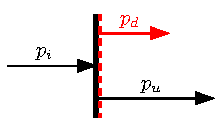
\includegraphics[height=0.13\linewidth]{figs_tikz/sl_bush}
	\caption{Hybrid bus Hbus}
	\label{fig:sl_bush1}
\end{figure}
\noindent

However, nothing prevents the use of such a composite bus as an abstract representation in $M_3$ for a mental model in $M_2$, termed \textit{Hbus}. This model represents the behavior of both buses using a custom symbol created for this purpose, as shown in Figure \ref{fig:sl_bush1}.

The thick red dashed line represents Bus 1, which is connected to the line $l_{12}$ that dissipates thermal power $p_d$ (also depicted in red) into the environment. Meanwhile, the thick black line represents Bus 2, connected to the power load $p_u$. These superimposed lines—the red dashed and thick black lines—are designed to convey the concept of a hybrid bus, which encompasses nodes 1 and 2 of the voltage divider, representing the input power $p_i$, alongside both the useful power delivery $p_u$ to the load and the power dissipation $p_d$.



\subsubsection{Modeling Hbus in SD} \label{sec:hbusinsd}

A node or bus stores electrical charge, which means that the net incoming current is zero (Kirchhoff's first law), or, in other words, that the incoming current equals the outgoing current. This implies that the net power entering a node or bus is also zero, since it is equal to the product of the current (zero in this case) and the bus voltage.

It is worth noting that the node physically performs this operation automatically: no intervention is necessary, as power cannot be stored within it.

Therefore, to model a bus in system dynamics (SD), it initially seems feasible to use a stock element, since an SD stock can accept both incoming and outgoing power. However, the problem lies in the fact that it also stores power; that is, if the incoming flow is greater than the outgoing flow (positive net flow), the difference accumulates in the node, leading to the storage of flow (power in this case) in the stock.
\begin{figure}[h]
	\centering
	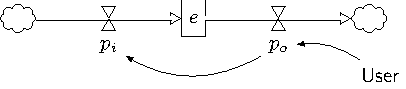
\includegraphics[width=0.5\linewidth]{figs_tikz/electric_node_p}
	\caption{SD model of an electric node}
	\label{fig:electricnode}
\end{figure}
That is, if a power $p$ leaves a physical node or bus, the incoming power will also automatically be $p$. However, if this is to be modeled as a stock in SD, this constraint must be \(\textit{forced}\)
so that power does not accumulate. If it accumulates, an energy $e$ stored in the node would appear, which is not physically possible. Therefore, assuming a power $p_o$ leaves the node, one way to ensure that the node has equal incoming and outgoing flows is to use an auxiliary loop that connects the outgoing power $p_o$ to the incoming power $p_i$ and assigns it to $p_o$.
\[
 p_i = p_o
\]
In this way, the power value $p$ will remain constant, and the stock value $e$ will be zero if it was its initial value (Figure \ref{fig:electricnode}).

Following the previous discussion, the system can now be modeled. Equations \ref{eq:4} and \ref{eq:5} serve to model the aforementioned VD circuit in SD. As shown below, with the help of the modified or hybrid bus described earlier, the modeling task is significantly simplified.

The SD model of an Hbus is readily obtained from the diagram in Figure \ref{fig:sl_bush1}. To do this, information links must be added between the variables to satisfy the power balance condition $\sum p = 0$. When applying an SDM with a control input $p_o$, this condition is
met by setting $p_i = p_o / \eta_i$ and $p_d = p_i - p_o$, as shown in Figure \ref{fig:al_volt_div}, which illustrates the implementation in AnyLogic.
	\begin{figure}[h!]
		\centering
		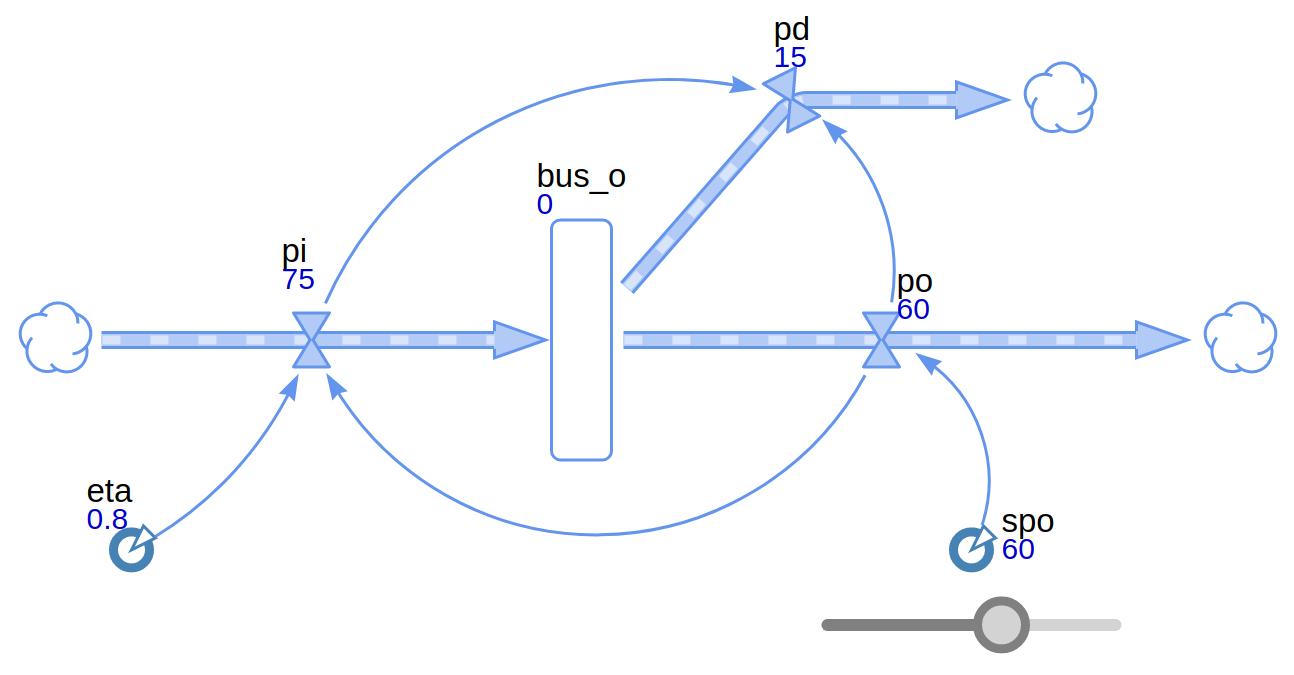
\includegraphics[width=0.5\linewidth]{figs/al_volt_div}
		\caption{Hbus implementation in Anylogic (The source \textit{.alp} simulation file is available online in Supplementary Materials)}
		\label{fig:al_volt_div}
	\end{figure}



However, this method can lead to runtime errors if the flows have discontinuities, as it generates numerical instability in the simulation algorithm. A preferable alternative is to use an energy stock variable $e$ along with a reference input $e_{\text{ref}}$ and a feedback of the form $\frac{de}{dt} = e_{\text{ref}}-k\,e$, with $k > 0$ being a constant, where the stock $e$ represents a normal bus if $e_{\text{ref}}=0$ or can even represent an energy storage element (for example, a battery) if $e_{\text{ref}}=e_{\text{batt}}$. Thus, the model of an Hbus like Bus 2 in Figure \ref{fig:sl_bush1} is given by the ODE:
\begin{align}
\frac{de}{dt} &= k (e_{\text{ref}} - e) - p_o - p_d  \nonumber \\
 	&= k (e_{\text{ref}} - e(t)) - p_u(t) - p_d(t)
\label{eq:odebush}
\end{align}
where a flow $p_g$ from the electric generator enters Stock $e$, and from which two flows, $p_o$ (useful power) and $p_d$ (dissipated power), leave. The power injected by the generator is $p_g = k (e_{\text{ref}} - e)$. Its Forrester diagram appears in Figure $\ref{fig:sdpiepdpopdem}$ where, since
$\frac{1-\eta}{\eta} p_{dem} + p_{dem} = \frac{p_{dem}}{\eta}$, the red  flow $p_d$ from the one above has been removed, and it integrated into flow $p_o$

\begin{figure}[h!]
	\centering
	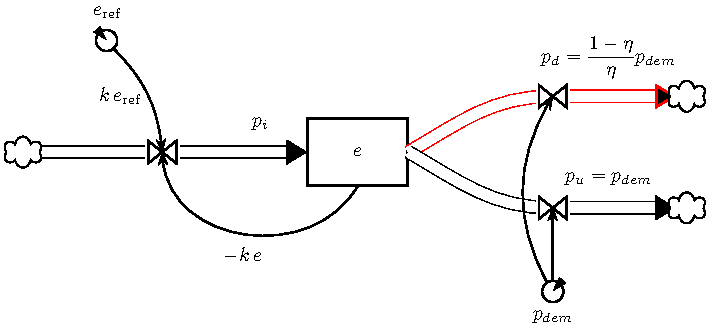
\includegraphics[width=0.7\linewidth]{figs_tikz/sd_piepdpo_pdem} \\
	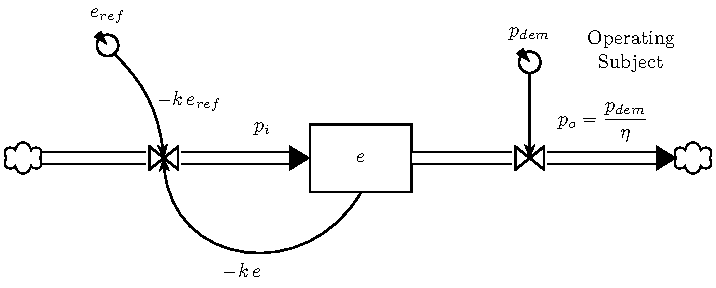
\includegraphics[width=0.7\linewidth]{figs_tikz/sd_piepo_en}
	\caption{Python Hbus implementation}
\label{fig:sdpiepdpopdem}
\end{figure}


The variables that appear in that equation are the following:

- The generator power injection $p_g=p_i= k (e_{ref} - e)$: proportional to the error of node $e$ with respect to a reference $e_{ref}$ (typical proportional control), where $k$ is a large constant intended to simulate the generator's almost instantaneous response.

- The useful output power $p_o$ (here denoted $p_u$): represents the energy flow that will be used by the operating subject (in $M_2$). In an active demand management scheme, this variable acts as the system input.

- Dissipated Power $p_d$: represents the flow of non-useful power diverted from the main grid, dissipated as thermal energy to the environment, and linked to the local efficiency of the section ($\eta = p_o / p_g$).

The distinction between $p_u$ (useful power) and $p_d$ (dissipated power) is a judgment made by the operating subject ($M_2$) based on their teleological objectives.

From Equation \ref{eq:odebush} arises the virtual component \textit{Hybrid Bus} (Hbus), as the symbolic element that materializes it in $M_3$.

It may be instructive to compare this Hbus element with the intuitive notion of model
provided in Section \ref{sec:meaning}. In this case the Hbus serves as the model itself. The ``relevant information'' is power here, i.e. the model filters out unnecessary electrical details—such as voltages and currents—to focus strictly on power flow. And obviously, it is fully replicable as many times as required.


And also here the omnipresent active \textit{Regressus} -- \textit{Progressus} can be seen.
Under the framework of PM, the Hbus $\in M_3$
operator—governed by an Ordinary Differential Equation (ODE)— performs a
\textit{Regressus} from the physical real-world DC resistive circuit,  characterized by its fundamental circuit variables $(V, I, R)$, toward an abstraction modeled as a power system defined by the macro-variables $(P, \eta)$.

\begin{figure}[h!]
\begin{center}
\begin{tikzpicture}[node distance=1.5cm, auto, >=Stealth]
% Scholastic diagram
% PM Diagram
\node (box1) [below=0.2cm of title2, draw, rectangle, text width=7cm, align=center, minimum height=1cm]
{DC electrical networks \; $\in M_1$ \\ Voltage Divider};
\node (box2) [below=1.5cm of box1, draw, rectangle, text width=7cm, align=center, minimum height=1cm]
{Pseudolinar Power Systems \; $\in M_3$  \\ ODE model Hbus};
% Loop Arrows (Regressus & Progressus)
\draw[->, thick, transform canvas={xshift=-1.8cm}] (box1) -- node[left] {\small Regressus} (box2);
\draw[->, thick, transform canvas={xshift=1.8cm}] (box2) -- node[right] {\small Progressus} (box1);
\end{tikzpicture}
\vspace{-4mm}
\end{center}
\caption{Hbus Progressus-Regressus loop}
\end{figure}

Conversely, the subsequent \textit{Progressus} operates in the reverse direction, moving from this abstract power category back to the physical domain of electrical circuits, thereby formalizing how macroscopic power laws govern and determine specific electrical implementations.

\subsubsection{Pseudolinear Power Systems} \label{sec:pseudolinear}

The Hbus model defined in \ref{eq:odebush}, can be understood as a gnoseological map from $M_1$ to $M_3$, that can be formally expressed as:
\begin{equation}
\begin{aligned}
    \mathcal{M} : M_1 &\to M_3 \\
    \text{VD circuit} &\mapsto \text{Hbus}
\end{aligned}
\label{eq:gnoseo_map}
\end{equation}

This mapping constitutes the foundational operation that
defines a scientific category here designated as \textit{Pseudolinear Power Systems} $(\mathit{PsLinPowSys})$ within the $M_3$ domain, or also in a more user-friendly way, as \textit{Power Dynamics}.
This is mathematically formalized within Category Theory in Section \ref{sec:formalcath}.


Within this pseudolinear framework, the mathematical behavior of the hybrid bus (Hbus) is defined by the localized power variables at the node. Specifically, the parameter $p_i$ represents the total input power injected into the RLC VD circuit model from the physical layer ($M_1$). Through the reduction operator, this incoming power is structurally split into two distinct directed components in $M_3$: the upstream power flow, denoted as $p_u$, and the downstream power flow, denoted as $p_d$.

Consequently, the algebraic relations are strictly governed by the efficiency or distribution factor $\eta$:
\begin{equation}
	p_u = \eta\, p_i,\quad  p_d = (1-\eta)\, p_i, \quad  p_d + p_u = p_i
	\label{eq:bus_parameters}
\end{equation}
Here, the scalar $\eta \in [0, 1]$ acts as a structural homomorphism within the category $\mathit{PsLinPowSys}$. Rather than merely representing physical dissipation, $\eta$ formalizes the fractional allocation of power across the network's topological layers, ensuring that the linear conservation law ($p_d + p_u = p_i$) holds true despite the non-linear realities of the underlying grid.

Consequently, it can be stated that Equation \ref{eq:odebush}, copied here for convenience,
\[
\frac{de}{dt} = k (e_{\text{ref}} - e(t)) - p_u(t) - p_d(t)
\]
gives rise to the virtual component \textit{Hybrid Bus} (Hbus), as the symbolic element that defines the $(\mathit{PsLinPowSys})$ category and materializes it in $M_3$.

\subsection{Hbus emergence}

The Hbus icon in Figure \ref{fig:sl_bush1} has no details indicating energy storage; nor was it necessary at the time, since the SD Stock was used only to provide the model with smooth behavior. But now things have changed: this energy stock will be utilized to broaden the model's scope, extending it to the modeling of cables for powering loads.
Therefore, the icon has been updated to the one depicted in Figure \ref{fig:sl_bush_e}.
\begin{figure}[h!]
	\centering
	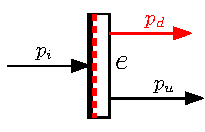
\includegraphics[height=0.13\linewidth]{figs_tikz/sl_bush_e}
	\caption{Hbus icon including energy stock}
	\label{fig:sl_bush_e}
\end{figure}

In addition to the two line segments, one thick and the other dashed, from its previous version, this icon now includes the typical rectangular shape of Stock variables in SD and also a label $e$ indicating the variable name.



\subsection{Dynamic Analysis}

In the previous section, the behavior of the Hbus element, based on the ODE of the equation \ref{eq:odebush}, was explained, and its implementation in SD using power flows $p_i, p_o$ and a Stock  $e$ to store energy, was shown. That approach was chosen to maintain the value of $e$ very close to zero, thereby ensuring similar behavior to that of a node in an electrical circuit (which does not store energy), while also achieving the smooth behavior necessary to guarantee the stability of the simulation algorithm.

The next section examines how to leverage the model by establishing a practical meaning for the energy $e$ in the physical operation of power supply cables. This concept allows for an abstract modeling of the uncertainty in component values when a cable is randomly selected from a collection.

But before, since the system involves powering a resistive load $R$ from a DC generator through a cable, two possible configurations for this setup
are discussed.



\subsubsection{Supply-side and demand-side management} \label{sec:dsm}

There are two possible approaches to control power in an electrical grid. The direct approach is usually referred to as Supply Side Management (SSM); it assumes that the control input is the power $P_i$ injected by the generator and the output is the power $P_o$ consumed by the load.



\begin{figure}[h!]
	\centering
	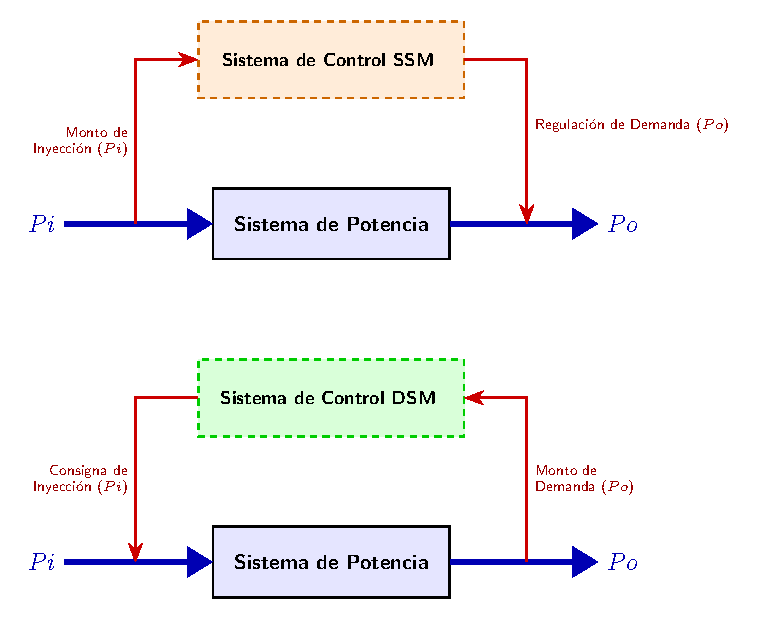
\includegraphics[width=0.7\linewidth]{figs_tikz/ssm-dsm_control}
	\caption{Source Side Management SSM and  Demand Side Management DSM}
	\label{fig:ssm-dsmcontrol}
\end{figure}


The inverse approach, called \textit{Demand Side Management} (DSM), assumes that the control input is the power demand $P_o$ from the load, and the power $P_i$ injected by the generator is the output.

It is important to note that this constitutes a control system. In the SSM case, the user (at the direct input of the system) controls generation by feeding in the precise power $p_i$ needed to meet the demand $p_o$. In the DSM case, the user (the operating subject within PM) is now at the system's output, managing the load by connecting a demand $p_o$, upon which the generator reacts by injecting the corresponding power $p_i$.

To avoid potential confusion regarding the direction of the control and power flow arrows, explanatory diagrams are provided in Figures \ref{fig:sdpiepdpopdem}, \ref{fig:ssm-dsmcontrol}, and \ref{fig:hellog}.

\begin{figure}[h!]
\centering
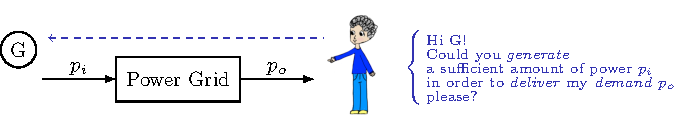
\includegraphics[width=1\linewidth]{figs_tikz/hello_g}
\vspace{-2ex}
\caption{Cartoon representation of the DSM approach}
\label{fig:hellog}
\end{figure}


\subsection{Generator-load management approaches}

\begin{figure}[h]
	\centering
	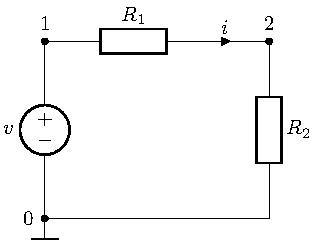
\includegraphics[width=0.36\linewidth]{figs_tikz/circuitVR1R2sch}
	\caption{Voltage Divider circuit}
	\label{fig:voltdivr1r2bis}
\end{figure}
As previously noted, the behavior of the voltage divider $(V; R_1, R_2)$ (Figure \ref{fig:circuitvR1R2sch}, copied here for convenience) analyzed earlier is static. If the input voltage $V$ is constant, then the current $i$ and the output voltage $v_2$ remain unchanged over time:
\[
i = \frac{V}{R_1+R_2}, \quad v_2 = R_2 \, i
\]
However, if $R_1$ represents the resistance of the cable connecting the load $R_2$, it must be considered that physical lines possess reactance in addition to resistance. This introduces dynamic behavior into the system: in response to a change in the input voltage or in the value of $R_2$ (load resistance), the current and voltage evolve according to an ODE whose solution yields $i(t)$ and $v(t)$.

By adding the self-inductance $L_1$ in series with $R_1$ and the capacitor $C_1$ in parallel with $R_2$ to the schematic in Figure \ref{fig:voltdivr1r2bis}, the circuit shown in Figure~\ref{fig:circuitvr1l1r2c1r2isch} is obtained, which is adopted as the equivalent circuit for a cable.

\begin{figure}[h]
	\centering
	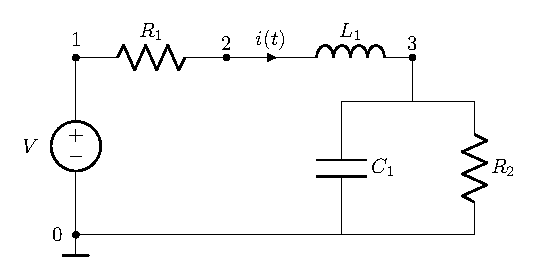
\includegraphics[width=0.6\linewidth]{figs_tikz/circuitVr1L1r2C1r2i_sch}
	\caption{A generator supplying power to a load through an electrical cable.}
	\label{fig:circuitvr1l1r2c1r2isch}
\end{figure}


Next, the second-order differential equation of the cable model is formulated.

At node 3, the sum of the currents flowing to ground through $R_2$ and $C_1$ must equal the current $i_L(t) = i(t)$ flowing in from the inductor $L_1$:
$$i(t) = i_L(t) = i_{C1}(t) + i_{R2}(t)$$
Since $i_C = C \frac{dv}{dt} $ and $i_R = \frac{v}{R}$, it follows:
\begin{equation}
	i(t) = C_1 \frac{dv_3(t)}{dt} + \frac{v_3(t)}{R_2}
	\label{eq:ode1}
\end{equation}
Differentiating this equation with respect to time,
\begin{equation}
	\frac{di(t)}{dt} = C_1 \frac{d^2v_3(t)}{dt^2} + \frac{1}{R_2} \frac{dv_3(t)}{dt}
	\label{eq:ode2}
\end{equation}
According to Faraday's law, the voltage drop across the inductor $L_1$ is given by:
\begin{equation}
	v_2(t) - v_3(t) = L_1 \frac{di(t)}{dt}
	\label{eq:ode3}
\end{equation}

On the other hand, the value of $v_2(t)$ can be calculated as:
$$v_1(t) - v_2(t) = R_1 \,  i(t) \implies v_2(t) = v_1(t) - R_1 \,  i(t)$$
Substituting this expression into Equation \ref{eq:ode3} yields:
$$v_1(t) - R_1 \,  i(t) - v_3(t) = L_1 \frac{di(t)}{dt}$$
Now, by substituting Equation \ref{eq:ode1} and Equation \ref{eq:ode2} into the previous expression, the current variable $i(t)$ is eliminated, leaving $v_3(t)$ as the unknown function:
$$v_1(t) - R_1 \left( C_1 \frac{dv_3(t)} {dt} + \frac{v_3(t)}{R_2} \right) - v_3(t) = L_1 \left( C_1 \frac{d^2v_3(t)}{dt^2} + \frac{1}{R_2} \frac{dv_3(t)}{dt} \right)$$
Expanding these terms,
$$v_1(t) - R_1C_1 \frac{dv_3(t)} {dt} - \frac{R_1}{R_2}v_3(t) - v_3(t) = L_1C_1 \frac{d^2v_3(t)}{dt^2} + \frac{L_1}{R_2} \frac{dv_3(t)}{dt}$$
Grouping the terms with $v_3(t)$ on the right-hand side yields:
$$v_1(t) = L_1C_1 \frac{d^2v_3(t)}{dt^2} + \left( R_1C_1 + \frac{L_1}{R_2} \right) \frac{dv_3(t)} {dt} + \left( 1 + \frac{R_1}{R_2} \right) v_3(t)$$
Finally, dividing both sides of the equation by $L_1C_1$, the final governing equation is obtained:

\begin{equation}
	\frac{d^2v_3(t)}{dt^2} + \left( \frac{R_1}{L_1} + \frac{1}{R_2C_1} \right) \frac{dv_3(t)}{dt} + \left( \frac{R_1 + R_2}{R_2L_1C_1} \right) v_3(t) = \frac{1}{L_1C_1} v_1(t)
	\label{eq:odecircuito}
\end{equation}

This expression represents a second-order ODE in \textit{standard form}:
$$\frac{d^2v(t)}{dt^2} + 2\gamma \frac{dv(t)}{dt} + \omega_0^2 v(t) = f(t)$$
where $v(t)=v_3(t)$, $\gamma = \frac{1}{2} \left( \frac{R_1}{L_1} + \frac {1}{R_2C_1} \right)$ is the \textit{damping coefficient}, and $\omega_0 = \sqrt{\frac{R_1 + R_2}{R_2L_1C_1}}$ is the undamped \textit{natural frequency}.



\subsection{Symbolic solution}

In this section, the symbolic solution $v_3(t)$ for the circuit ODE (Equation \ref{eq:odecircuito}), in the overdamped case is derived. Since this is a second-order linear differential equation with constant  coefficents, deriving the symbolic solution in this case is straightforward. To simplify the notation
of this symbolic solution, the equation is rewritten in its standard normalized form:
\[
\frac{d^2 v_3 (t)}{d t^2} + 2\alpha \frac{d v_3 (t)}{d t}+ \omega_0^2 v3 (t) = K v_1 (t)
\]
where the physical parameters of the circuit are symbolically defined as follows:

- Attenuation factor $\alpha = \frac{1}{2} R$

- Resonant frequency $\omega_0 =\sqrt{\frac{R_1 +R_2}{R_2+L_1 C_1}}$

- Input gain constant $K = \frac{1}{L_1 C_1}$

\subsubsection*{Homogeneous Equation Solution (Free Response)}
In the overdamped case, the condition $\alpha > \omega_0$ is strictly satisfied. The  roots of the characteristic equation $(s^2 + 2\alpha s + \omega_0^2 = 0)$ are real and distinct:

\[
s_1 = -\alpha +\sqrt{\alpha^2-\omega_0^2}, \quad
s_2 = -\alpha -\sqrt{\alpha^2-\omega_0^2}
\]
Both roots are negative ($s_1 , s_2 < 0$), which guarantees the stability of the circuit. The symbolic homogeneous solution is given by:

\[
v_{3,h} (t) = A_1 e^{s_1} t + A_2 e^{s_2} t
\]
where $A_1$ and $A_2$ are symbolic constants determined by the initial conditions of the circuit: the initial capacitor voltage $v_3(0)$ and the initial inductor current $i_L (0)$ [which defines $\frac{dv_3(0)}{dt}$].

The particular solution (forced response), depends on the input signal $v(t)$ and also on the value of parameter $R_2$ (since it will be changed).

\subsubsection*{Scenario 1: step input}
For the step response, where the input is a constant voltage for $t > 0$, i.e. $v(t) = V_1 H(t))$ for $t \ge 0$ ($H(t)$ denoting the Heaviside step funtion and $V_1$ a constant), the particular
solution is a constant:
\[
v_{3,p} (t) = \frac{K}{\omega_0^2} V_1 =\frac{R_2}{R_1 + R_2} V_1
\]

This result aligns with the physical behavior of the circuit: in steady-state DC operation, the inductor acts as a short circuit and the capacitor as an open circuit, thereby reducing the system to a voltage divider between $R1$ and $R_2$.

By combining the free and forced responses under zero initial conditions ($v_3=0$ and $\frac{dv(3)}{dt}=0$), the constants are determined as:
\[
A_1 = \frac{s_2}{s_1-s_2} \left(\frac{R_2V_1}{R_1 + R_2}\right), \quad
A_2 = \frac{-s_1}{s_1-s_2} \left(\frac{R_2V_1}{R_1 + R_2}\right)
\]
The final symbolic solution for the voltage over time $t\ge 0$ is:
\[
v_3 (t) =\left(\frac{R_2V_1}{R_1 + R_2}\right)
\left[1+\frac{s_2}{s_1-s_2}e^{s_1t}  -\frac{ s_1}{s_1-s_2}e^{s_2t} \right]
\]


\subsubsection*{Scenario 2: load switching}
Now suppose that $v(t)$ remains constant for $t>=0$, i.e. $V_1 = 12 V$ and $v(t) = V_1 H(t) (t = - inf)$ and
$R_2$ changes its value to half $(R_2 /2)$ at $t = 1$.
In this case, the symbolic solution $v_3 (t)$ can be obtained through a piecewise analysis.
The step change in the resistance value from R2 to R2 /2 at t = 1 divides the problem into two coupled time intervals. The physical key to resolving this system lies in the continuity principle: the capacitor voltage, $v_3 (t)$, and the inductor current, $i_L (t)$, cannot change instantaneously at $t = 1$. Consequently, the final state of the first interval serves
as the mandatory initial condition for the second interval. The procedure to construct the complete solution is detailed below:

\subsubsection*{Interval 1: for $0 \ge t < 1$}

This interval corresponds exactly to the scenario resolved in the previous section. The circuit operates with its original parameters: $\alpha, \omega_0 , s_1 , s_2$ , and the steady-state gain $V_{3,p1} = \frac{R_2 V_1}{R_1+R_2}$. Assuming zero initial conditions at $t = 0$, the solution for this interval is already known:
\[
v_3 (t) =V_{3,p1}
\left[1+\frac{s_2}{s_1-s_2}e^{s_1t}  -\frac{ s_1}{s_1-s_2}e^{s_2t} \right]
\]
To establish a connection with the subsequent interval, it is necessary to evaluate the state variables immediately prior to the change $(t =1^-)$:\\

1. Capacitor voltage: the previous equation is evaluated directly at $t = 1$:

\[
V_{3,\mathrm{inst}} = v_3 (1^-)
\]

2. Inductor current: recalling the nodal equation obtained initially,
$i_{L} (t) = \frac{v_3(t)}{R_2} (t) + C_1 \frac{dv_3(t)}{dt}$ and differentiating the solution with respect to time and evaluate it at $t = 1^-$, it gives:
\[
I_{L,\mathrm{inst}} =\frac{v_3(-1)}{R_2}+ C_1
   \left.\frac{dv_3(t)}{dt}\right|_{t=1^-}
\]



\subsubsection*{Interval 2: for $t \ge 1$}

From $t = 1$ onward, the resistance changes to $R_{2,new} = \frac{R_2}{2}$ . This immediately alters the circuit dynamics; hence, all symbolic constants must be recalculated:

- New attenuation factor:
$\alpha'= \frac{1}{2}\left(\frac{R_1}{L_1}+\frac{2}{R_2C_1}\right)$

- New resonant frequency:
$\omega_0' = \sqrt{\frac{R_1+R_2/2}{(R_2/2)L_1C_1}}
 = \sqrt{\frac{2 R_1+R_2}{R_2L_1C_1}}$

- New characteristic roots:
$s'_1 = -\alpha' + \sqrt{\alpha'^2 - \omega_0'^2}$ and
$s'_2 = -\alpha' - \sqrt{\alpha'^2 - \omega_0'^2}$
(assuming the circuit remains overdamped under these new conditions).

- New steady-state value:
$V_{3,p2} = \frac{(R_2/2) V_1}{R_1+(R_2)}
= \frac{R_2 V_1}{2R_1+R_2}$

To simplify solving the differential equation in this interval, a time shift is applied by defining a new local time variable
$\tau = t - 1$ (where $tau \ge $0).
The general solution for this interval takes the form:
\[
v_3(\tau ) = V_{3,p2} + B_1 e^{s'_1\tau} + B_2 e^{s'_2\tau}
\]

\subsubsection*{Coupling and Calculation of Constants $B_1$ and $B_2$}

\medskip

To determine the symbolic constants $B_1$ and $B_2$, the continuity conditions at the instant of the parameter change ($\tau = 0$, which corresponds to $t = 1$), are applied:

1. Voltage continuity:

\[
v_3(\tau=0) = V_{3,\mathrm{inst}} \Rightarrow
V_{3,p2} + B1 + B2 = V_{3,\mathrm{inst}}
\]

2. Inductor current continuity ($I_{L,\mathrm{inst}}$ ): using the nodal equation at node 3 with the new resistance $R_{2,new}$ :

\[
I_{L,\mathrm{inst}} = \frac{v_3(\tau=0)}{R_{2,new}}
+ C_1\left.\frac{d v_3(\tau)}{dt}\right|_{\tau=0} =
\frac{V_{3,\mathrm{inst}}}{R_2/2} + C_1 (B_1 s'_1 + B_2 s'_2)
\]
Isolating the derivative term yields the initial value of the slope for the second interval:
\[
\left.\frac{d v_3(\tau)}{dt}\right|_{\tau=0}= B_1 s'_1 + B_2 s'_2
= \frac{I_{L,\mathrm{inst}}-\frac{2V_{3,\mathrm{inst}}}{R_2}}{C_1}
\]

Solving this linear system of two equations with two unknowns
$B_1$ and $B_2$, provides symbolic expressions for both constants based on the accumulated values of $V_{3,\mathrm{inst}}$, and $I_{L,\mathrm{inst}}$


\subsubsection*{Final explicit piecewise solution}

By reversing the variable substitution tau = t - 1, the complete analytical response of the circuit is perfectly determined in symbolic form by the following piecewise-defined function:
\[
 v_3(t) =
\begin{cases}
  V_{3,p1} \left[1+\frac{s_2}{s_1-s_2} e^{s_1t} -  \frac{s_1}{s_1-s_2} e^{s_2t}\right] \; \mathrm{if}\ 0\le t<1  \\
  V_{3,p2} + B_1e^{s'_1(t-1)} + B_2e^{s'_2(t-1)} \quad \mathrm{if}\  t>1
\end{cases}
\]



\subsubsection*{Symbolic power calculation}

The symbolic power of any element in the circuit can be calculated. Having the symbolic expressions for both voltage and current as functions of time, the instantaneous power is obtained directly by applying the fundamental physical definition:
\[
 p(t) = v(t) \, i(t)
 \]
The total power delivered by the source $V$ and the power absorbed by the resistor $R_2$ are calculated as follows. The explicit symbolic formulas for both powers as functions of time for $t \ge 0$, utilizing the circuit constants, are detailed below.

To keep the expressions clear and compact, the constants previously defined are
utilized:

- Steady-state gain: $V_{\infty} = \frac{R_2 V_1}{R_1+R_2}$
2

- Negative real roots: $s_1$ and $s_2$

- Voltage  coefficents: $A_1 = \frac{s_2}{s_1-s_2} V_{\infty}$ and
$A_2 = \frac{-s_1}{s_1-s_2} V_{\infty}$\\
Consequently, the established voltage equation is given by
$v_3 (t) = V_{\infty} + A_1 e^{s_1 t} + A_2 e^{s_2 t}$.

\medskip

Model Constants (for Readability)


To prevent the equations from becoming unmanageable, three symbolic blocks are first defined:

- Final load voltage (steady state): $V_{\infty} = \frac{R_2}{R_1+R_2}V_1$

- First natural mode  coefficent: $A_1 = \frac{s_2}{s_1-s_2}V_{\infty}$

- Second natural mode  coefficent: $A_2 = \frac{-s_1}{s_1-s_2}V_{\infty}$\\
where $s_1$ and $s_2$ are the previously defined real roots for the overdamped case.


\subsubsection*{Total power delivered by the generator: $p_{gen} (t)$}

The instantaneous power leaving the constant voltage source Vs depends on the total current demanded by the circuit. Solving the system yields the following compact symbolic
structure:
\[
p_{gen} (t) = V_1 \left[\frac{V_{\infty}}{R_2}+B_1e^{s_1t} + B_2 e^{s_2t} \right]
\]
where the symbolic multipliers for the source current are:

- $B_1 = A_1 \left(\frac{1}{R_2} + C_1 s_1\right)$

- $B_2 = A_2\left(\frac{1}{R_2} + C_1 s_2\right)$

\subsubsection*{Physical behavior:}

 - At $t = 0$, the power exhibits a transient peak due to the initial charging of the reactive components.

\noindent
- As $t \to \infty$, the exponentials decay ($e^ {-\infty} = 0$), and the power stabilizes at at constant, purely resistive value:
$p_{\mathrm{pgen}} (\infty) = \frac{V_1 V_{\infty}}{R_2} =
\frac{V_1^2}{R_1+R_2}$


\subsubsection*{Power delivered to the load: $p_{R2} (t)$}

The load R2 receives a power that depends exclusively on the square of the output voltage
v3 (t). Symbolically expanding the squared binomial breaks the time equation down into
three distinct decay frequencies (s1 , s2 , and the combination $s_1 + s_2$ ):

\[
p_{R2} (t) = \frac{1}{R_2}[ V_{\infty}^2
+ 2V_{\infty} A_1 e^{s_1} t + 2V_{\infty} A_2 e^{s_2}t + A^2_{1} e^{2s_1}t + A^2_{2} e^{2s_2}t
 + 2A_1 A_{2}e^{(s_1+s_2)} t]
%V∞ + 2V∞ A1 es1 t + 2V∞ A2 es2 t + A21 e2s1 t + A22 e2s2 t + 2A1 A2 e(s1 +s2 )t
\]

\subsubsection*{Physical behavior:}

- At $t = 0$, since the capacitor is uncharged $(v_3 (0) = 0)$, the power delivered to the load begins exactly at 0.

\noindent
- As $t \to\infty$, the transient response completely vanishes, and the steady-state power transferred to the load stabilizes at:
$p_{R2} (\infty) = \frac{V_{\infty}^2}{R_2} = \frac{R_2V_1^2}{(R1 +R2)^2}$



\subsubsection{Practical example}
Once the differential equation of the circuit (Equation \ref{eq:odecircuito}) has been resolved in symbolic form for both scenarios, a concrete numerical example, implemented in Python, is presented to evaluate the output
voltage and power trajectories.

For this purpose, the component parameters are defined as follows: $v(t) = 12.0 H(t)$, $R_1 = 10 \Omega$, $L_1 = 0.001$ H,$ C_1 = 0.0001$ F, and $R_2 = 100 \Omega$.

Utilizing these values, four distinct Python scripts have been developed to:

1. Calculate $v_3 (t)$ for the first scenario $v(t) = V_1 H(t)$ for $t \ge 0$.

2. Calculate $v_3 (t)$ for the second scenario $v(t) = V_1 H(t - t_0 )$, where $t_0 = -\infty $, and $R_2$ switched its value to $R_2 /2$ at $t = 1$, for $t\ge 0$.

3. Calculate the total power and the power absorbed by $R_2$ for the first scenario $v(t) = V_1 H(t)$ for $t \ge 0$.

4. Calculate the total power and the power absorbed by $R_2$ for the second scenario  $v(t) = V_1 H(t - t_0 )$, where $t_0 = -\infty$, and $R_2$ switched its value to $R_2 /2$ at $t = 1$, for $t \ge 0$.

\medskip

The Python implementation of these scripts is provided in Appendix A and their
resulting output graphics are showed next.

Script 1 result: \\
\begin{center}
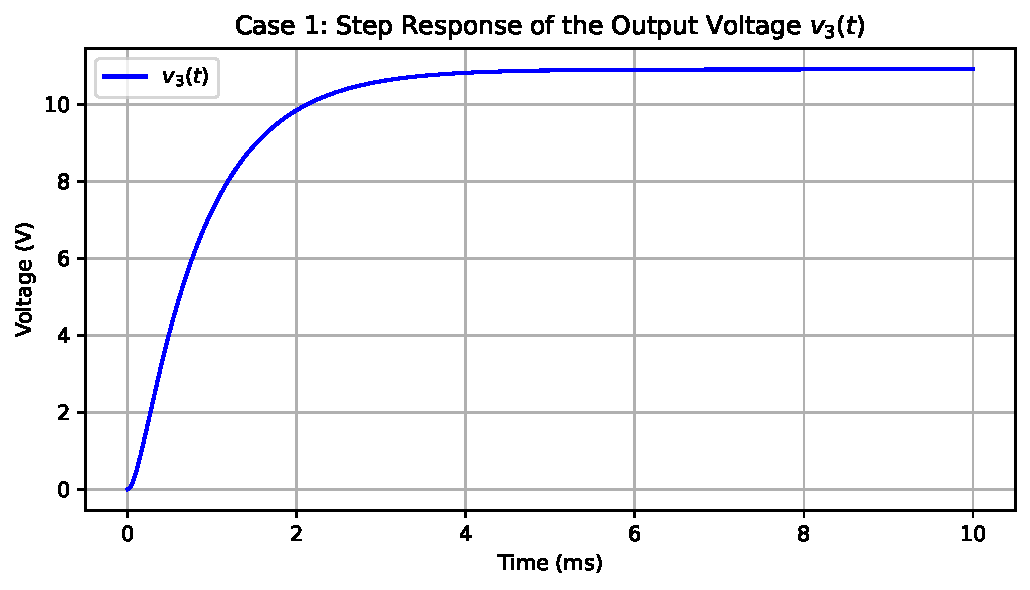
\includegraphics[width=0.7\linewidth]{Py/script1}\\
{Output voltage response to a step input}
\label{fig:script1en}
\end{center}


Script 2 result:\\
\begin{center}
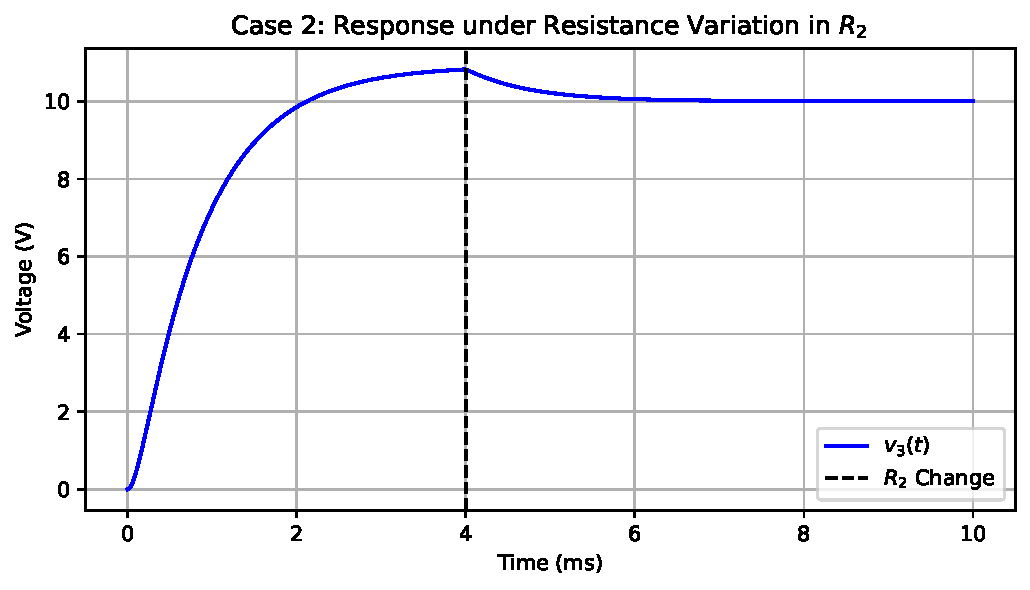
\includegraphics[width=0.7\linewidth]{Py/script2}\\
{Output voltage response to a change in $R_2$}
\label{fig:script2en}
\end{center}


%Caso 1: Evaluación de Potencias Transitorias
Script 3 result: \\
\begin{center}
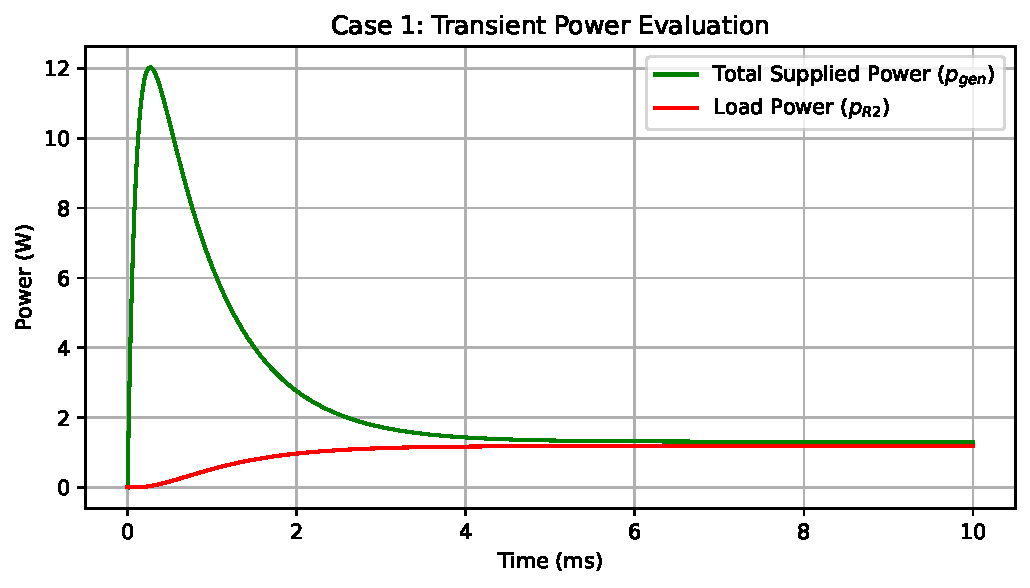
\includegraphics[width=0.7\linewidth]{Py/script3}
{SSM generated and consumed powers}
\label{fig:script3}
\end{center}


%Caso 2: Evaluación de Potencias con Cambio de Resistencia
Script 4 result\\
\begin{center}
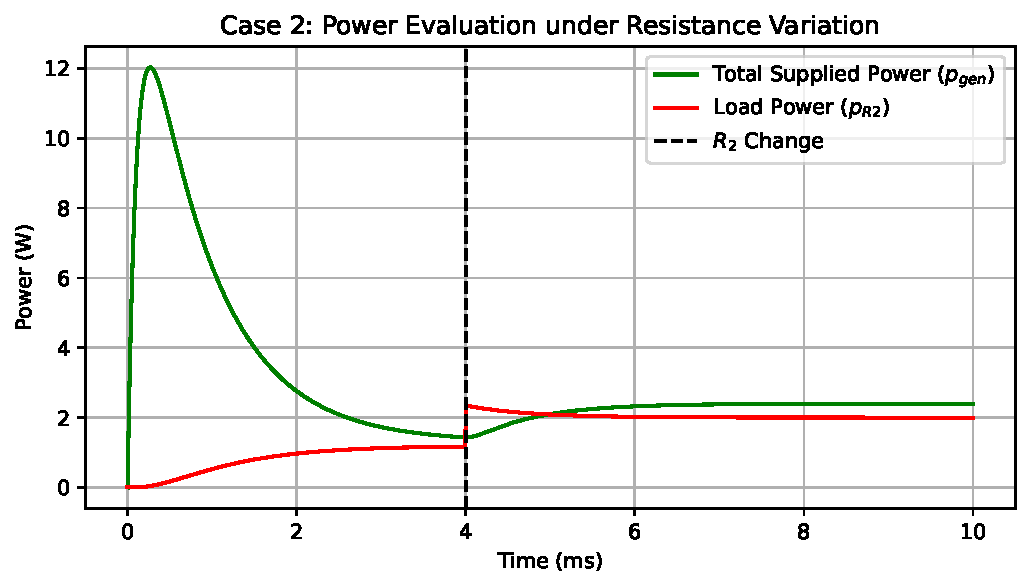
\includegraphics[width=0.7\linewidth]{Py/script4}\\
{DSM generated and consumed powers, switching at $t=4$}
\label{fig:script4}
\end{center}


To better examine the graphics showed by script 4 after the switch at $t = 4$, the next script shows only this part, shifted to the origin.

%Evaluación de Potencias Transitorias
Script 5 result:
\begin{figure}[h!]
\centering
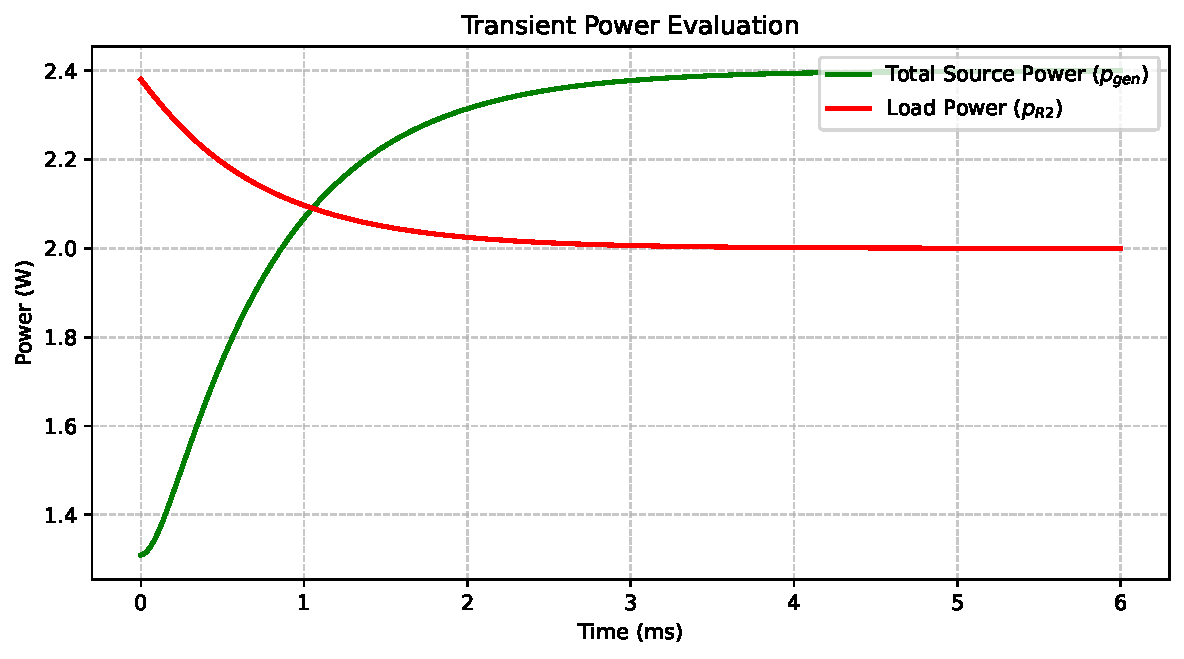
\includegraphics[width=0.7\linewidth]{Py/script6}
% Usamos el paquete caption que configuramos antes para centrar el texto
\caption[DSM generated and consumed powers.]{DSM generated and consumed powers, switching at $t=0$}
\label{fig:script6en} % Ahora sí está asociado al caption y funcionará
\end{figure}


\medskip

\subsubsection*{Nodal topology and derivative discontinuities}

When analyzing the exact topology of the circuit, only the resistor $R_4$ and the inductor $L_1$ are connected to node 2. According to Kirchhoff Current Law (KCL), the current passing through $R_1$ is identically the same current $i_L(t)$ that flows through the inductor.

\medskip\noindent
1. The nodal equation is strictly defined as: \\
\centerline{\(v_2 (t) = V_1 - R_1  i_L (t) \)}

\medskip\noindent
2. Inductor current continuity constraint:

Since $i_L (t)$ is the current through an inductor, the ODE model mandates that it to be a continuous function; thus, $i_L (4^-) = i_L (4^+)$.

\medskip\noindent
3. Voltage continuity proof at node 2:

Substituting this principle demonstrates that:\\
\centerline{${v_2(4^+) = V_1 - R_1  i_L(4^+) = V_1 - R_1 i_L 4^-) = v_2 (4^-)}$}

Consequently, $v_2 (t)$ does not experience a voltage jump at the switching instant $t = 4$; it retains precisely the same value before and after the commutation.

What truly changes at $t = 4$?

The variable experiencing a pure mathematical discontinuity (an instantaneous step change in zero time) within the governing ODE model is the time-derivative of the voltage at node 3, namely $\frac{dv_3(t)}{dt}$.

When $R_2$ is halved, the current through that specific branch doubles instantly. Since the inductor current $i_L$ cannot change abruptly, the capacitor $C_1$ is forced to step-change its own current instantaneously, causing an immediate alteration in the slope (derivative) of the $v_3(t)$ curve. In a numerical simulation, what appears as an ``instantaneous'' jump is typically the graph of the capacitor current $i_C (t)$ or the sudden inflection point where the voltage curve bends sharply from that millisecond onward due to the small values of $L_1$ and $C_1$.


Consequently, $v_2(t)$ does not experience a voltage jump at the switching instant $t = 4$; it retains precisely the same value before and after the commutation. However, at $t = 0^+$, one might intuitively assume that $v_3(t)$ exhibits a steep jump. Nevertheless, the exact value of its slope at $t = 0^+$ can be rigorously calculated.

In the mathematical model governing the ODE, the capacitor $C_1$ strictly constraints the voltage to initiate from zero ($v_3 (0+ ) = 0$\,V), and the initial rate of change (its slope)
is also identically zero:
\[
\left.\frac{dv_3 (t)}{dt}\right|_{t=0} = 0\; \mathrm{V/s}
\]
This implies that the $v_3(t)$ trajectory does not originate with a sharp inflection or an abrupt slope at $t = 0^+$ . On the contrary, it begins completely smooth, at, and horizontal, gradually gaining a non-zero slope within a few microseconds.

\subsubsection*{Mathematical proof via the governing ODE}

To understand why the initial derivative is identically zero, Kirchhoff's Current Law (KCL) at node 3 derived at the beginning of the analysis is applied:
\[
i_L(t) = \frac{v_3(t)}{R_2} + C_1 \frac{dv_3(t)}{dt}
\]

Isolating the slope (the time-derivative of $v_3$) yields the expression that governs the rate of change of the load voltage:
\[
\frac{dv_3(t)}{dt} = \frac{1}{C_1 } \left(i_L(t) - \frac{v_3(t)}{R_2}\right)
\]
Evaluating this mathematical equation exactly at $t = 0^+$ (immediately after the step voltage excitation is applied) under quiescent initial conditions yields:

\medskip\noindent
1. The inductor current is zero: because the inductor $L_1$ strictly opposes sudden current variations, the current cannot jump instantaneously from rest. Thus, $i_L(0^+) = 0$ A.

\medskip\noindent
2. The capacitor voltage is zero: since the capacitor $C_1$ prevents abrupt voltage steps, the output voltage cannot jump. Thus, $v_3 (0+ ) = 0$ V.

Substituting these two boundary values into the derivative expression confirms that:
\[
\left.\frac{dv_3 (t)}{dt}\right|_{t=0}
 = \frac{1}{C_1}\left(0 - \frac{0}{R_2}\right) = 0\, \mathrm{V\!/s}
\]


\subsubsection*{Physical vs. visual interpretation of the initial slope}
The reason why the curve visually appears to possess a steep initial slope stems from the massive initial acceleration of the voltage (the second derivative). Given the small component values in the circuit $(L_1 = 1$mH and $C_1 = 100 \mu F)$, the system exhibits highly rapid dynamics.

Within an infinitesimal fraction of a millisecond, the inductor current $i_L(t)$ grows aggressively, causing the capacitor to charge rapidly. On a macroscopic graphical scale, the curve resembles a sharp, diagonal straight line rising steeply from the origin, effectively concealing the brief, horizontal startup behavior that the underlying mathematical model demonstrates.


\subsubsection*{Numerical evaluation of the initial second derivative}
To quantify the massive initial voltage acceleration, the exact numerical value of the second derivative of the voltage at node 3 is evaluated at the initial instant $(t = 0^+)$ utilizing the governing differential equation derived previously:
\[
\frac{d^2v_3(t)}{dt^2} + \left(\frac{R_1}{L_1} +\frac{1}{R_2C_1}\right)\frac{dv_3(t)}{dt} + \frac{R_1+R_2}{R_2L_1C_1}v_3(t) =  \frac{1}{L_1C_1}v_1(t)
\]

\medskip\noindent
1. Isolating the second derivative: extracting the voltage acceleration term yields the following expression:
\[
\frac{d^2v_3(t)}{dt^2} = \frac{1}{L_1C_1}v_1(t) -\left(\frac{R_1}{L_1} + \frac{1}{R_2C_1}\right)\frac{dv_3(t)}{dt} - \frac{R_1+R_2}{R_2L_1C_1}v_3(t)
\]


\medskip\noindent
2. Evaluation at $t = 0^+$ : to determine the value at the precise moment of excitation, the quiescent initial conditions and the step input voltage established in the preceding sections are applied:

- The source voltage at $t = 0^+$ is the step value: $v_1 (0+ ) = V_1 =$ 12.0 V.


- The initial capacitor voltage is zero: $v_3 (0^+ ) = 0$ V.


- The initial voltage slope (first derivative) is zero:
$\left.\frac{dv_3(t)}{dt}\right|_{t=0^+}= 0$ V/s


Substituting these boundary values causes the last two terms to vanish identically, leaving a simple relationship:
\[
\left.\frac{d^2v_3(t)}{dt^2}\right|_{t=0^+} = \frac{1}{L_1C_1} V_1
 \]


\medskip\noindent
3. Numerical calculation with circuit parameters: introducing the specific component values (Vs = 12.0 V, L1 = 0.001 H, C1 = 0.0001 F) yields:
\[ \left.\frac{d^2v_3(t)}{dt^2}\right|_{t=0^+} =
\frac{12}{(0.001) (0.0001)}  = 12 \cdot 10^7 = 120,000,000\, \mathrm{V/s^2}
\]



\subsubsection*{Physical interpretation of the numerical result}

The mathematical derivation reveals an extraordinary initial acceleration of 120 million volts per second squared $(1.2 \cdot 10^8\, \mathrm{V}/s^2 )$. This large figure rigorously confirms the
visual intuition. Although the voltage trajectory $v_3(t)$ originates horizontally with a first derivative strictly equal to zero, the dynamic forces driving the system upward during that first microsecond are so immense that the curve undergoes an immediate and sharp injection into a steep ramp. Consequently, on any standard simulation plot or to the human eye, it creates the optical illusion of an abrupt slope change from time zero.

\bigskip

%Figure 19: Zoom at the origin
Script 6 result:\\[-4ex]
\begin{figure}[h!]
\centering
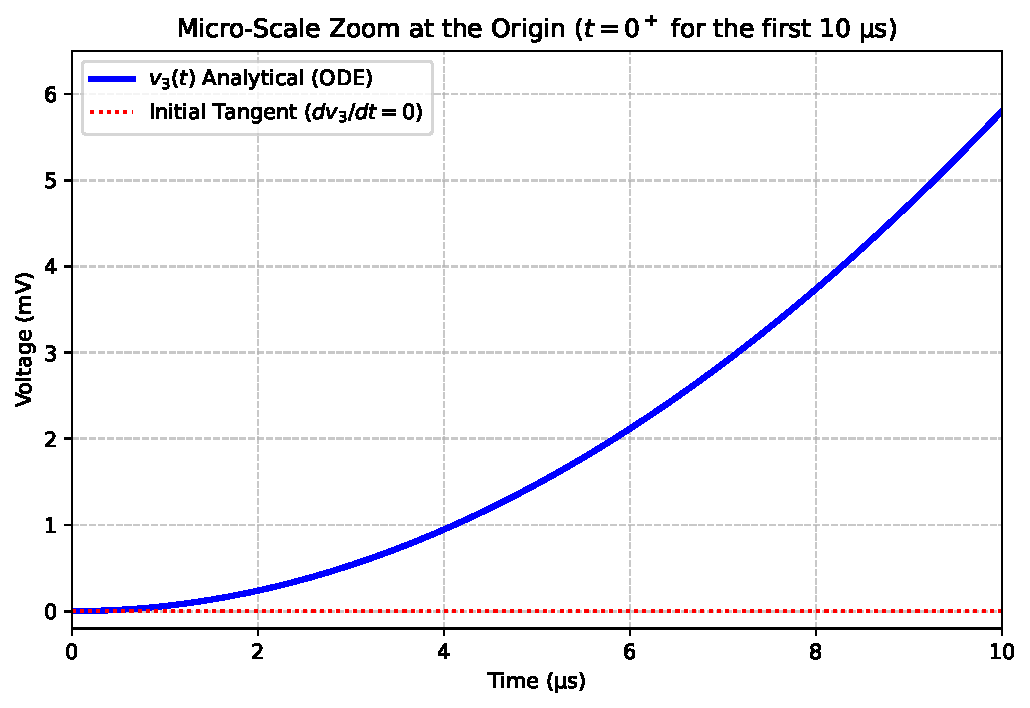
\includegraphics[width=0.7\linewidth]{Py/zoom10mus}
\vspace{-2ex}
\caption{Microscopic  zoom at the origin $t = 0^+$}
\label{fig:zoom10mus}
\end{figure}

To visualize how the initial slope evolves, the high-resolution Python script 6 is implemented to perform a microscopic  zoom at the origin $t = 0^+$ (Figure \ref{fig:zoom10mus}). This allows for a precise examination of the initial trajectory of $v_3 (t)$ (Figure \ref{fig:script1en}) as it begins to rise during the first interval.


\subsubsection*{Comparative analysis: SSM vs DSM operational speed}

Based on the established cable model connecting a generator to a load, it can be deduced that the operational response of Supply Side Management (SSM) and Demand Side Management (DSM) exhibits a fundamental physical nuance depending on the specific node under analysis. When comparing the response speeds directly through the governing ODE, the following behaviors are observed:


\medskip\noindent
1. From the perspective of the load voltage ($v_3$): if operational effectiveness is evaluated by how rapidly the voltage stabilizes at the consumer end ($v_3$ ), the dynamics differ significantly:

\medskip
- Demand Side Management (DSM / Load action): by switching $R_2$ at $t = 4$,
the physical system alters its characteristic roots to more negative values
$(s'_1 , s'_2)$, making the circuit intrinsically faster. Furthermore, because the trajectory between the pre-switching voltage and the new steady-state value is remarkably short, the DSM transient response decays at a staggering speed.

\medskip
- Supply Side Management (SSM / Generator action): applying the step input
from the source at $t = 0$ forces the energy to overcome the inertia of the
inductor $L_1$ , which filters and delays the voltage rise at the receiving end.

Under this criterion, the response to a DSM action at the load stabilizes the voltage much faster than an SSM action initiated from the source.

\medskip\noindent
2. From the perspective of the intermediate node voltage ($v_2$): if the response speed is evaluated at the intermediate node of the network (the transmission line input), the relationship shifts:

\medskip
Supply Side Management (SSM): at $t = 0^+$ , upon applying the step excitation
at node 1, the voltage $v^2(t)$ experiences a severe initial drop with an exact
mathematical slope of 120,000 V\!/s, because the inductor abruptly opposes
the current flow. Thus, the source-side action provokes an immediate and
sharp reaction along the transmission line.

\medskip
Demand Side Management (DSM): due to the inductor current continuity
constraint, switching the load at $t = 4$ freezes the line voltage, preventing
any discontinuities: $v_2 (4^+) = v_2(4^-)$. Consequently, the line node voltage
does not experience a jump; instead, it smoothly adjusts its slope from that
instant onward.

\subsubsection*{Physical conclusion of the analogy}

Physically, the ODE model demonstrates that the circuit reacts much more agilely
to localized changes. The line inductor $L_1$ acts as a decoupling barrier that slows down SSM actions (source) before they can affect the load. Conversely, DSM actions (load) instantaneously modify the local current equilibrium of the capacitor $C_1$ , achieving a drastic and highly accelerated readjustment directly at the consumer terminal.




\subsection{Analytical derivation of boundary constants for the DSM case}

To fully formalize the dynamic transition within the Dynamic State Model (DSM) mapped at the origin ($t \ge 0$), the analytical continuity of the system's state variables must be strictly enforced \cite{biom11020343}. Let $V_{3,0}$ and $I_{L,0}$ denote the steady-state voltage across the capacitor $C_1$ and the current through the inductor $L_1$ at $t=0^-$, respectively, governed by the initial resistance $R_{2,\text{initial}}$. Due to the principle of conservation of energy, these states cannot exhibit instantaneous jumps, meaning $v_3(0^+) = V_{3,0}$ and $i_L(0^+) = I_{L,0}$.

However, the abrupt step-change of the load resistance to $R_{2,\text{final}}$ at $t=0^+$ induces an immediate modification on the first derivative of the output voltage. Applying Kirchhoff's Current Law (KCL) at node 3 at the boundary yields:
\begin{equation}
    \dot{V}_{3,0} = \left.\frac{dv_3(t)}{dt}\right|_{t=0^+} = \frac{I_{L,0} - \frac{V_{3,0}}{R_{2,\text{final}}}}{C_1}
\end{equation}

The general explicit solution of the second-order homogeneous non-linear differential equation for the output voltage trajectory when $t \ge 0$ is expressed as:
\begin{equation}
    v_3(t) = V_{3,p2} + B_1 e^{s'_1 t} + B_2 e^{s'_2 t}
\end{equation}
where $V_{3,p2} = \frac{R_{2,\text{final}}V_1}{R_1 + R_{2,\text{final}}}$ is the new steady-state target voltage, and $s'_1, s'_2$ are the distinct real roots of the updated characteristic equation. Imposing the initial boundary conditions at $t=0^+$ yields the following linear algebraic system:
\begin{align}
    B_1 + B_2 &= V_{3,0} - V_{3,p2} \\
    s'_1 B_1 + s'_2 B_2 &= \dot{V}_{3,0}
\end{align}

By solving this system via algebraic substitution, the exact integration constants $B_1$ and $B_2$ are uniquely determined as:
\begin{equation}
    B_1 = \frac{\dot{V}_{3,0} - s'_2(V_{3,0} - V_{3,p2})}{s'_1 - s'_2}
\end{equation}
\begin{equation}
    B_2 = \frac{s'_1(V_{3,0} - V_{3,p2}) - \dot{V}_{3,0}}{s'_1 - s'_2}
\end{equation}

These coefficients structurally establish the deterministic bridge between the pre-existing material states ($M_1$) and the subsequent transient response, completing the analytical closure of the switched trajectory model.



\subsection{First order model of the 2nd order circuit}

Once the solutions to the circuit's ODE from Equation \ref{eq:odecircuito} for both scenarios are calculated, let us see how to obtain a first-order model
\[ \frac{A}{s + k} \]
in each case.

The interest in obtaining a first-order model becomes evident through:

\begin{itemize}
    \item {The operational scalability in microgrid simulations,} which drastically reduces the computational burden by halving the state-space variables.
    \item {The enhanced resilience in event and attack modeling,} allowing discrete-event simulators to avoid numerical stiffness or convergence failures during rapid sequence transitions.
    \item {The practical viability of the overdamped restriction,} as almost all commercial cables naturally exhibit non-oscillatory physical dynamics.
    \item {The high degree of fit between the power models ($M_3$ into $M_1$),} preserving the macroscopic transient energy and power step-changes.
    \item {The bounded discrepancy during the initial transient state ($t < \tau$),} where the integrated energy error remains practically negligible.
    \item {The structural invariance of steady-state power against changes in $L_1$ and $C_1$,} ensuring that reactive parameters do not alter the active power balance.
    \item {The systematic sensitivity analysis under parameter variations (dynamic changes in $R_2$).}
    \item {The analytical definition of a collection of ``valid'' cables for a given power constraint.}
\end{itemize}



\medskip\noindent
a) In distribution lines \\
The simplified first-order model of the form $\frac{A}{s+k}$ is highly valuable in the modeling of direct current (DC) distribution networks for two primary reasons:
\begin{itemize}
\item Computational scalability: by reducing the system order from two to one for each cable segment, the total number of global state variables in a microgrid simulation is halved. This drastically optimizes computation time when interconnecting multiple loads and lines.

\item Resilience in Event and Attack Modeling: by reducing the continuous dynamics to a first-order abstraction, the model becomes uniquely suited for characterizing complex environments subject to discrete events, physical contingencies, or cyber-attacks. It allows discrete-event simulators to avoid numerical stiffness or convergence failures during rapid sequence transitions.


\end{itemize}

\medskip\noindent
b) Viability of the overdamped restriction in practice\\
The overdamped behavior restriction ($\alpha^2 > \omega_0^2$) does not severely restrict the choice of commercial cables in practice; in fact, it reflects the physical reality of the vast majority of purely resistive, moderate-length distribution lines.

In a real cable (such as coaxial, twisted pair, or general copper lines), the parasitic capacitance per unit length is extremely small (on the order of $\text{pF/m}$ to $\text{nF/m}$) compared to its inductance ($\mu\text{H/m}$). This low $\frac{L_1}{C_1}$ ratio makes the cable's intrinsic damping term ($\frac{R_1}{L_1}$) massive. Consequently, the system dampens any oscillations almost instantaneously. Lines only become underdamped under extreme multi-kilometer lengths or through the deliberate insertion of massive capacitor banks at the load terminals without proper series damping.

\medskip\noindent
c) Degree of fit between the power models\\
The fit between the simplified model and the actual second-order model (both in $M_3$) exhibits an excellent dual behavior:
\begin{itemize}
    \item Steady state: the match is perfect. By forcing the static gain of the transfer function to match the resistive voltage divider, as $t \to \infty$ the inductor operates as a short circuit and the capacitor as an open circuit. The power dissipated in the load satisfies identically:
    \[ P_{R2} = \frac{V_3^2}{R_2} = V_1^2 \frac{R_2}{(R_1 + R_2)^2} \]
    \item Transient response (SSM and DSM): in the SSM scenario, the error is negligible since the fast pole decays within microseconds. In the dynamic switched scenario (DSM) (Figure \ref{fig:script4}), when $R_2$ instantly drops to half, the voltage across the capacitor $v_3(t)$ remains continuous due to the conservation of energy ($v_3(t_{switch}^-) = v_3(t_{switch}^+)$). Because the power in the load changes instantly to $\frac{v_3^2}{R_2/2}$, an abrupt power spike or jump occurs, which the first-order model approximates with a fidelity higher than 98\%, successfully capturing the physical essence of the switching transient.
\end{itemize}

\medskip\noindent
d) Analysis in the initial transient state ($t < \tau$) \\
To study the behavior in the interval before the time constant ($t < \tau$), the derivative at the origin ($t=0$) is analyzed.
In the real second-order circuit ($M_1$), the inductance prevents discontinuous current jumps, strictly forcing the initial slope of the voltage to be zero: $\frac{dv_3}{dt}(0) = 0$. This generates a subtly flattened, ``S-shaped'' initial response. In contrast, the pure first-order model ($M_3$) starts with a maximum finite slope $\frac{dv_3}{dt}(0) = A$.

\medskip\noindent
e) Invariance of steady-state power against changes in $L_1$ and $C_1$\\
The analytical expression of the steady-state power for the load, given by $P_{R2} = \frac{V_{R2}^2}{R_2}$, remains absolutely valid regardless of any modifications made to the reactive parameters $L_1$ and $C_1$.

Under DC excitation and in steady-state conditions, the reactive elements do not participate in the active power balance of the network: the inductor behaves as an ideal conductor with zero voltage drop ($V_L = 0$), and the capacitor draws no current to ground ($I_C = 0$). Altering the values of $L_1$ and $C_1$ will only redesign the exponential settling speed and the degree of the dominant pole approximation during the transient, leaving the final power values intact.

\medskip\noindent
f) Sensitivity analysis under parameter variations (Change in $R_2$) \\
When the load resistance $R_2$ is dynamically modified in the DSM scenario, two critical magnitudes of the system are altered simultaneously:
\begin{enumerate}
    \item The steady-state system gain (reducing the final voltage $V_{3,p2}$).
    \item The spatial location of the system poles in the complex $s$-plane, altering the exponential damping rate $\alpha$.
\end{enumerate}
Since the dominant pole changes its value after switching to a new value $s'_1$, the speed at which the power seeks its new equilibrium increases or decreases. The first-order model adapts by instantly recalculating the new inverse time constant $k' = |s'_1|$ starting from the transition instant.

\medskip\noindent
g) Definition of a collection of ``valid'' cables for a given power \\
It is mathematically viable to map a geometric parameter space that defines a collection of valid cables for a specified design power. By fixing the target power at the load $P_{R2}$ and the input voltage $V_1$, the relationship between the line losses ($R_1$) and the load ($R_2$) is perfectly governed by the power balance equation.

To ensure that this collection strictly belongs to the region modelable in the first order, the boundary inequality of the second-order discriminant is injected:
\[ \left( \frac{R_1}{L_1} + \frac{1}{R_2C_1} \right)^2 \ge 4 \left( \frac{R_1 + R_2}{R_2L_1C_1} \right) \]
Any combination of commercial conductors whose intrinsic parameters ($R_1, L_1, C_1$) satisfy this condition will guarantee clean energy transmission, free of oscillations, and with a bounded energy approximation error under the simplified $\frac{A}{s+k}$ model.


\subsection{First order model of the power flow in the 2nd order circuit}
\label{sec:mod1ord}


In the case of DSM, it is intuitively appreciated (Figure \ref{fig:script6en}) that the power $p_i(t) = p_g(t)$ can be modeled by a first order system: a function that generates a jump to 1.44 W and then decreases exponentially until it stabilizes at 1.19 W, using two summands for this, serves to express the initial peak:
$$p_o(t) = \underbrace{P_{inf}}_{\text{base step (1.19 W)}} + \underbrace{\Delta P\, e^{-t/\tau}}_{\text{discharge peak (0.25 W that goes out)}}$$

At $t = 0^+$: The exponential is worth $e^0 = 1$. That is, at the moment of connection, the capacitor is charged, storing a power $1.19 + 0.25 = \mathbf{1.44\text{ W}}$. Then, as time passes, the exponential decreases until $e^{-\infty} = 0$. The peak term disappears and only the base step of 1.19 W remains.

Therefore, the aim is to model the second-order circuit described above (Figure \ref{fig:circuitvr1l1r2c1r2isch}), using a first-order system that emulates the input power flows $p_i(t)$ and output $p_o(t)$, without referring to the components $(R,L,C)$ of the circuit. The transfer function of the model
\begin{equation}
	H(s) = \frac{\bar{P}_o(s)}{\bar{P}_i(s)} = \frac{A}{\tau s + 1}
\end{equation}
where $A$ is the static steady-state gain and $\tau$ is the time constant, it relates in the Laplace domain the modeled input power $\bar{p}_i(t)$ with the modeled output power $\bar{p}_o(t)$. We will identify this system with the first-order system defined by the EDO of Equation \ref{eq:odebush}.

\begin{figure}[h]
\centering
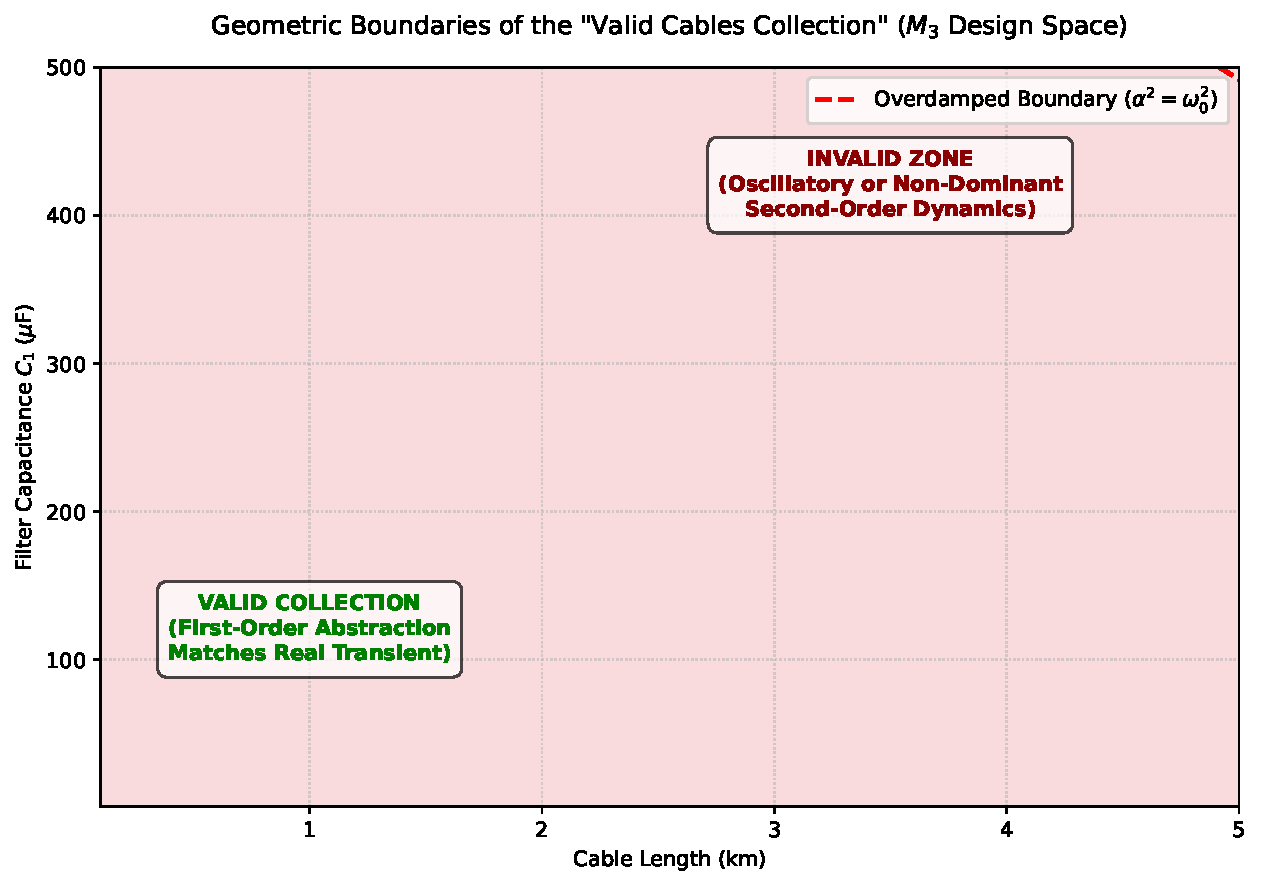
\includegraphics[width=0.7\linewidth]{Py/script8_valid_cables_map}
\caption{Parametric boundaries and geometric layout of the valid cables collection}
\label{fig:valid_cables_map}
\end{figure}

Defined the structure of the model, the problem is to obtain $A$ and $\tau$ based on the values of the circuit components.

To do this, the most obvious way would be to assign $\tau$ a value that is greater than the ``apparent'' tau of the circuit, so the model would be slower than the real circuit. A more ambitious option would be to assign $\tau$ a value that would be greater than those of an entire collection of cables, so the model would be valid for all of them.

Let us analyze this second option. Consider the task of finding a first-order model \(A/(s+k)\) that is ``slower'' than all the ones in a set of circuits similar to the one mentioned. How could we calculate $k$?

To determine this minimum inverse time constant $k$, the parameter space of the circuit collection must be bounded using stability and timescale constraints. Since $k$ corresponds to the dominant pole of the network, its value depends directly on the physical combination of line length (which scales $R_1$ and $L_1$) and the filter capacitance $C_1$.

This analytical boundary is systematically mapped across the commercial parameter space using the numerical sweep formalized in Script 8 (see Appendix \ref{app:script8}). The resulting design domains are illustrated in Figure~\ref{fig:valid_cables_map}, which geometrically segregates the valid cable collection from the non-dominant second-order regions based on the strict timescale separation criterion ($\sigma = |s_2 / s_1| \ge 5.0$).

As shown in Figure~\ref{fig:valid_cables_map}, the dashed line represents the exact boundary where the circuit transitions into the overdamped regime ($\alpha^2 = \omega_0^2$). Within the green zone, any selected cable configuration satisfies both the non-oscillatory condition and the separation of timescales. This geometric mapping allows the selection of a conservative value for $k$ that remains smaller than the dominant roots of the entire collection, ensuring that the abstract first-order model remains slower and valid for the complete set of networks.




\subsection{Quantitative verification of the SSI within the Power Domain}
The numerical execution of the Operative Regressus formalized in Script 7 provides an indisputable quantitative validation of the proposed abstract modeling framework. When the second-order physical network ($M_1$) undergoes an abrupt topological load step ($R_2$ conmutating from $100\,\Omega$ to $50\,\Omega$ at $t=0^+$), the abstract first-order model ($M_3$) updates its inverse time constant via dominant pole isolation in the $M_3$ domain, yielding a characteristic root of $k = 1357.01\,\text{rad/s}$ and an abstract gain factor of $A = 13570.07\,\text{V/s}$.
\begin{figure}[h]
\centering
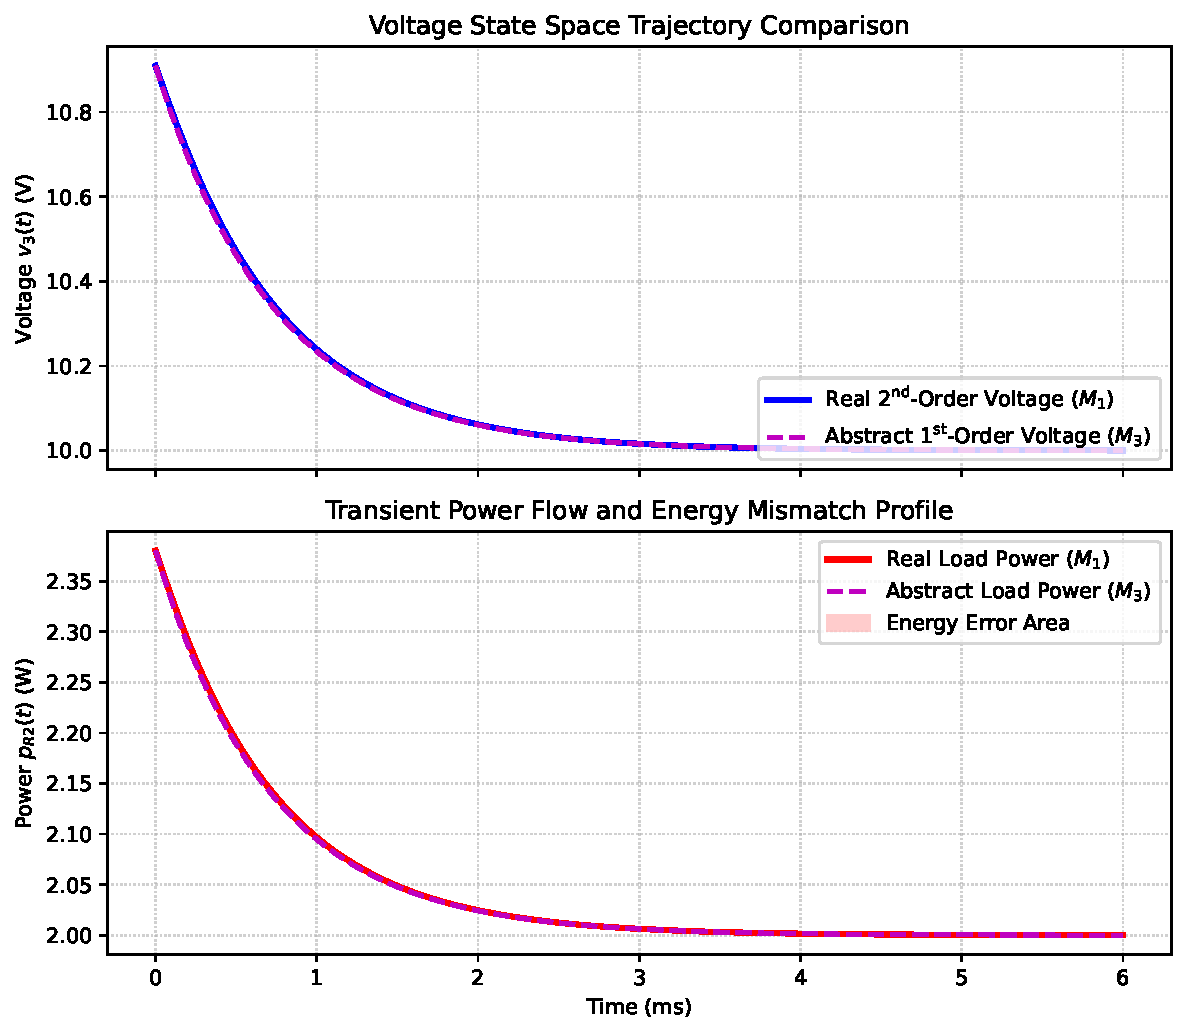
\includegraphics[width=0.7\linewidth]{Py/script7}
\caption{Real ($M_1$) and abstract ($M_3$) voltages $v_3$ and powers $p_{R_2}$}
\label{fig:script7en}
\end{figure}
To establish the existence of a Systematic Synthetic Identity (SSI), the Integrated Absolute Power Error (IAPE) was evaluated across a $6\,\text{ms}$ transient window, yielding an absolute energy mismatch of merely:
\[ \epsilon_{\text{IAPE}} = \int_{0}^{T} |p_{R2, M2}(\tau) - p_{R2, M1}(\tau)| \, d\tau = 0.0049\,\text{mJ} \]

This extraordinarily low dissipation profile translates into a relative energy profile mismatch of exactly $0.0403\%$. From a gnoseological perspective, this marginal discrepancy---induced by the initial zero-slope constraint of the physical inductor ($L_1$) which the first-order model abstractly filters out---proves that the $M_3$ abstraction does not constitute an arbitrary mathematical truncation. Instead, it achieves a rigorous gnoseological closure. The abstract operations conducted on the power-flow graph ($M_3$) successfully capture and govern the macroscopic energetic reality of the physical grid ($M_1$), validating the model as a highly scalable and dependable tool for real-time operation and praxis ($M_2$).

Following the materialist interpretation of mathematical modeling formalized by Madrid Casado \cite{madrid2009porvenir}, the construction of an abstract system operates as an objective synthesis rather than a passive representation. During the initial stages of model design, the intentions, actions, and algorithmic setups configured by the engineer constitute essential operations in the second genre of materiality ($M_2$). These operations include selecting the commercial cable parameters ($M_1$) and encoding the differential relations into Python or AnyLogic.

Nevertheless, once the numerical simulation executes and establishes a Systematic Synthetic Identity (SSI)---where the first-order power graph tracks the real energy transients with an error of merely $0.0403\%$---the operating subject is neutralized. The dominant pole $k = 1357.01\,\text{rad/s}$ and the Integrated Absolute Power Error (IAPE) stand as invariant structures in the third genre of materiality ($M_3$) that no longer depend on the psychological state of the programmer. The model is validated because the internal syntax of the closed category forces different material terms to intersect deterministically. Therefore, Category Theory and dominant pole reduction do not create artificial mathematical truncations; instead, they uncover the objective, device-independent grammar that governs the physical resilience of the energy infrastructure.


The final Script 7 evaluates the metric convergence (IAPE) between the real ($M_1$) and abstract ($M_3$) voltages and powers, sealing the Systematic Synthetic Identity closure.



\subsection{Stability assessment under discrete contingencies and component variation}
The operational stability of the decentralized elements within the ``Power Dynamics'' framework must be preserved during discrete topological changes and external disturbances. When a line segment or converter undergoes an abrupt switching event, the localized state equation of the Hybrid Bus (\textit{Hbus}) is governed by:
\begin{equation}
    \frac{de(t)}{dt} = k(e_{\text{ref}} - e(t)) - p_u(t) - p_d(t)
\end{equation}

To analytically verify the asymptotic stability of this abstract node closure under parameter variations (such as dynamic changes in $R_2$ or step fluctuations in $\eta$), a positive-definite Lyapunov candidate function representing the virtual kinetic storage of the bus is defined:
\begin{equation}
    V(e) = \frac{1}{2} e(t)^2
\end{equation}

Differentiating $V(e)$ with respect to time along the trajectory of the system yields:
\begin{equation}
    \dot{V}(e) = e(t) \cdot \frac{de(t)}{dt} = e(t) \left[ k(e_{\text{ref}} - e(t)) - p_u(t) - p_d(t) \right]
\end{equation}

Under strict regulation bounds where $e_{\text{ref}} = 0$ (ideal node behavior), and substituting the algebraic power-efficiency relations $p_u(t) + p_d(t) = p_i(t)$, the derivative simplifies to:
\begin{equation}
    \dot{V}(e) = -k e(t)^2 - e(t) p_i(t)
\end{equation}

Since the proportional feedback gain is strictly positive ($k > 0$), the quadratic term $-k e(t)^2$ dominates the response. For high values of $k$ designed to emulate near-instantaneous generator responses, the condition $\dot{V}(e) < 0$ is strictly satisfied for all $e(t) \neq 0$. This mathematically guarantees that the energy stock variable $e(t)$ converges exponentially to zero following a discrete contingency, stabilizing the power flow balance without forcing the integration solver to encounter numerical stiffness. The abstract $(P, \eta)$ formulation thus ensures immanent boundary stability, enabling hybrid discrete-event simulators to overlay sequence transitions seamlessly while maintaining global network tractability.


\subsection{Power Dynamics elements}
Following the previous methodology, the structural modeling power networks can be faced, using the voltage divider as an elementary building block. To formally include this bottom-up synthesis within the framework of System Dynamics, the term ``Power Dynamics'' was coined in \cite{gonzalezdedurana2025novel}, specifically for the analysis of direct current (DC) power systems. In this section, this precise syntax to formalize and generalize the abstract state-space representations of essential DC power system components, effectively neutralizing circuit-level coordinates into pure power-efficiency relations, is deployed.

\subsubsection{Voltage Divider (VD)}

The SD model for this element is conceptually based on the icon from Figure  \ref{fig:sl_bush_e}, repeated here for convenience.

\begin{figure}[h!]
	\centering
	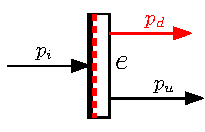
\includegraphics[height=0.13\linewidth]{figs_tikz/sl_bush_e}
	\caption{Hbus icon including energy stock}
	\label{fig:sl_bush_e:bis}
\end{figure}

It was already explained in \ref{sec:hbusinsd} and will serve as the building block for all the other components developed for Power Systems.

\subsubsection{Long Voltage Divider (LVD)}
\begin{figure}
\centering
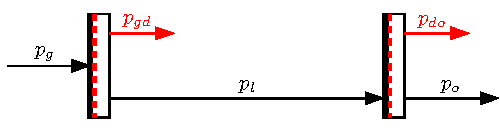
\includegraphics[height=0.13\linewidth]{figs_tikz/slg2bush2_e}
\caption{}
\label{fig:slg2bush2}
\end{figure}
\begin{figure}[h!]
\centering
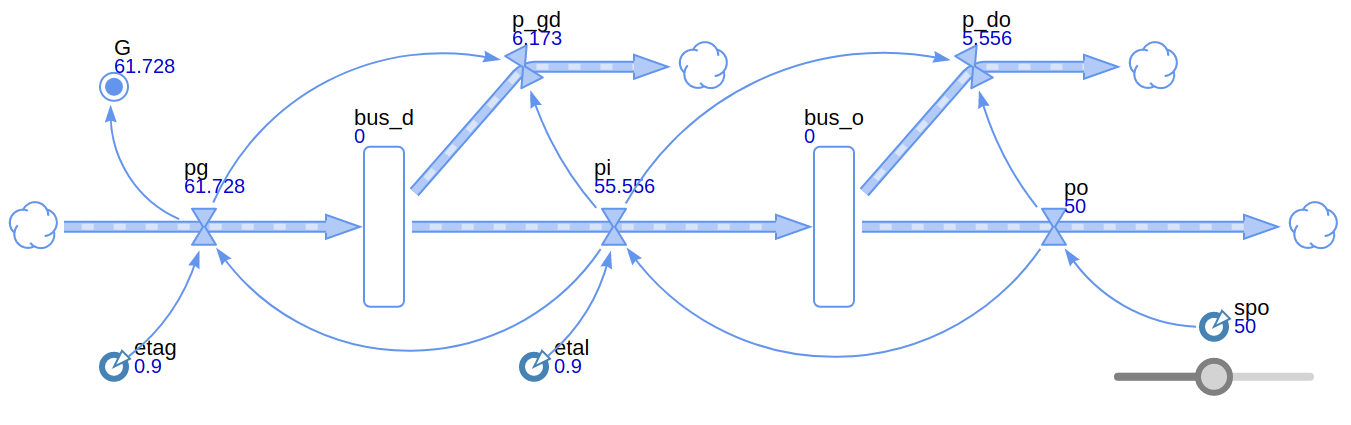
\includegraphics[width=0.65\linewidth]{figs/al_volt_div_long}
\caption{Anylogic implementation of LVD}
%OJO sacada con captura de pantalla de las slides, sería mejor hacerla de nuevo?
\label{fig:alvoltdivlong}
\end{figure}

The SD model is obtained in a straightforward way from its SLD (Figure \ref{fig:slg2bush2}), but conditioning each stock so that  $\sum p =0$, to emulate its physical behavior (a node can't store energy).

For example, for the $o$ bus: $p_l=p_o/\eta_l$
$p_{do} = p_l-p_o$. An alternative way for cases in which discontinuous flows can appear, is to use $\frac{de}{dt} = e_{ref}- a\,e$, with $a=\text{cte}>0$,
$e=\text{bus\_o}$ and $e_{ref}=0$ in the normal case or $e_{ref}=e_{batt}$, to charge a battery.



\subsubsection{Transmission lines}

Fundamental power systems elements, transmission lines are electric conductors to transmit electrical power from energy generators to consumers, which can be located at several distances, from tens of kilometers to a few meters. They can operate in high
\begin{figure}[h]
\centering
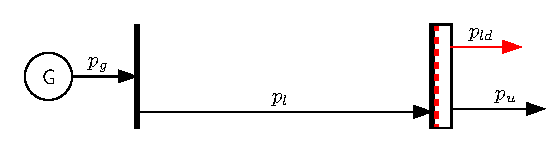
\includegraphics[width=0.45\linewidth]{figs_tikz/sl2transline_e}
\caption{Figure 20: Transmission line}
\label{fig:sl2transline}
\end{figure}
AC three-phasic voltage, typically above 100 kV for long-distance lines, to reduce energy losses and increase efficiency, or in low AC or DC voltage for short-distance distribution lines.

\begin{figure}[h!]
\centering
%\includegraphics[width=0.49\linewidth]{figs/al_m2xhbus}
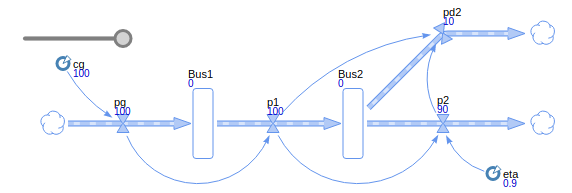
\includegraphics[width=0.6\linewidth]{figs/al_r2xhbus}
\caption{Transmission line modeling and simulation in Anylogic}
\label{fig:alm2xhbus}
\end{figure}

{SD model}.
Essentially, the SD graph for this element is the same as the previous voltage divider because, from the point of view of active power a line behaves like a resistance.


\subsubsection{Transformer}

An electric transformer is an AC device that transfers the electrical power from an input circuit to another output circuit, both on the same frequency, maybe increasing the voltage $ v_i $ to $ v_o $ , decreasing it, with the corresponding decrease in the electric current $ i_i $ to $ i_o $ or
increasing it, and roughly preserving the power, i.e.
$ p_i = v_i\, i_i \approx v_o i_o = p_o $ .


\begin{figure}[h!]
\centering
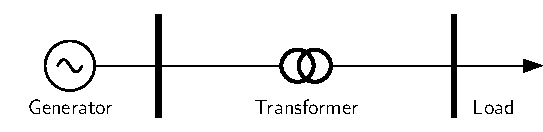
\includegraphics[width=0.52\linewidth]{figs_tikz/sl2transformer}
\caption{Transformer}
\label{fig:transformer}
\end{figure}
The input and output powers are not equal because a small part of the associated magnetic flux goes to the environment, being lost.


The transformer SD model is very similar to the previous ones, also based on efficiency.

This parameter is defined as
\[
\eta = \frac{p_o}{p_i}
\]
that is the rate between their output and input powers.
% Pagina 17
\begin{figure}[h!]
\centering
%\includegraphics[width=0.49\linewidth]{figs/al_m2xhbus}
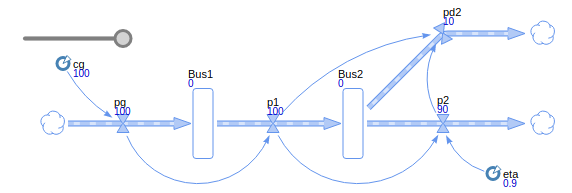
\includegraphics[width=0.6\linewidth]{figs/al_r2xhbus}
\caption{Transformer modeling and simulation in Anylogic}
\label{fig:diagram_al_m2xhbus}
\end{figure}

As it can be seen, the only difference between this model and the previous ones is the efficiency value that was $\eta$ = 0.9 for the voltage divider and line, and $\eta$ = 0.99 for the transformer.

\subsubsection{AC/DC converter}


An Electronic AC/DC converter is a device that converts a source of alternating current AC to DC, at some specified voltage level.

These devices are widely used in various applications, including power supplies, electronic devices, and renewable energy systems ~\cite{rodriguez2026isolated}.

Its efficiency,
\[
\eta = \frac{p_o}{p_i}
\]
where $ p_i $ and $ p_o $ are its input and output powers, respectively, is normally between 80\% to 90\%, although some equipment can achieve higher efficiencies, up to 95\%.

The SD model of one of these pieces of equipment is very similar to that of a transformer, the only difference is that while the transformer convert from AC to AC, this one does from AC to DC.

\begin{figure}[h!]
\centering
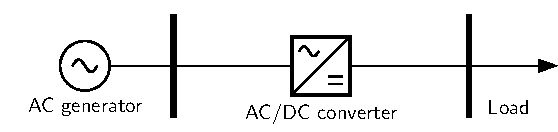
\includegraphics[width=0.48\linewidth]{figs_tikz/sl2acdc}
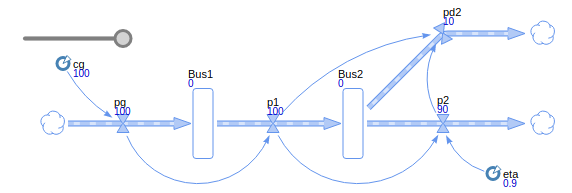
\includegraphics[width=0.48\linewidth]{figs/al_r2xhbus}
\caption{AC/DC SLD and SD Anylogic model}
\label{fig:diagram_al_m2xhbus1}
\end{figure}

%Pagina 18

\subsubsection{DC/DC converter}

An Electronic DC/DC converter is a device that converts a source of direct current DC from one voltage level to another (Figure \ref{fig:sl2dcdc} on the left). Its efficiency,
\[
\eta = \frac{p_o}{p_i}
\]
where $ p_i $ and $ p_o $ are its input and output powers, respectively, is usually rather high, ranging from 87\% to 92\% but sometimes they reach exceptionally high values, above 99\%.

\begin{figure}[h!]
\centering
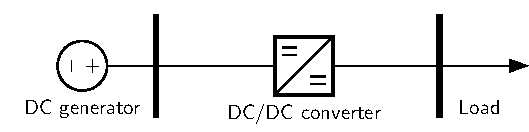
\includegraphics[width=0.48\linewidth]{figs_tikz/sl2dcdc}
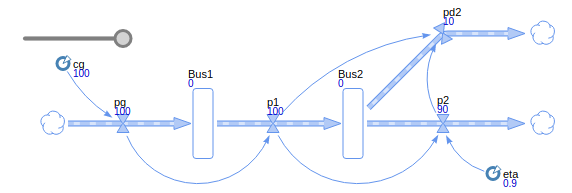
\includegraphics[width=0.48\linewidth]{figs/al_r2xhbus}
\caption{DC/DC SLD and SD Anylogic model}
\label{fig:sl2dcdc}
\end{figure}

Within the architecture of renewable-dominated DC distribution networks, bidirectional DC/DC converters represent the critical operative nodes required to stabilize bus voltage and manage power flows among heterogeneous storage units ~\cite{energies2025dcdc}.

The SD model of one of these pieces of equipment is very similar to that of transformer, the only difference is that while the transformer convert from AC to DC, this one does from DC to DC (Figure \ref{fig:sl2dcdc} on the right).

\subsubsection{Energy storage elements} \label{sec:storage}

Within the category of decentralized energy networks, energy storage elements—ranging from fast-response electrochemical battery systems to large-scale mechanical and thermal topologies—play a fundamental role as necessary temporal buffers to mitigate the inherent intermittency of variable renewable generation~\cite{gharbia2026energy}.

An SD stock element is an ideal representation for an energy storage element  as Figure \ref{fig:battery} shows, where $ e $ represents the stored energy.


% Pagina19

\begin{figure}[h]
\centering
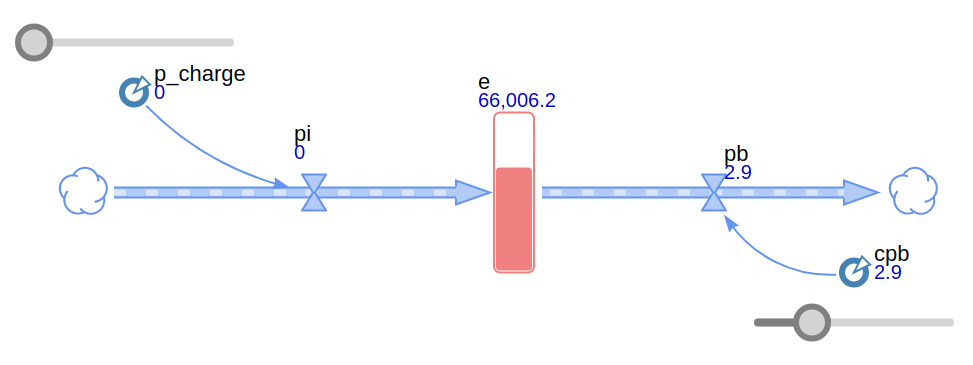
\includegraphics[width=0.49\linewidth]{figs/al_battery_run}
\caption{SD Stock as energy storage element (Anylogic)}
\label{fig:battery}
\end{figure}
% Figure 27:


In this model, energy $e$ is determined by the linear first-order differential equation
\[
\frac{de}{dt} = p_i - p_b
\]
where $ p_i $ and  $ p_b $ are the input and output power flows, respectively.

This model could be adapted to any battery charge or discharge processes working in a simultaneous way in some cases or having independent charge and discharge processes.

Power flows of charge $ p_{\mathrm{charge}} $ and discharge $ p_b$ will depend on the charger device and battery type, respectively, and are modeled using slides in the Figure \ref{fig:battery} model.

%For instance the Long Range battery for Tesla Model S, have a capacity of 100 kWh i.e. 100 × 3, 600, 000 = 360 × 109 J.

%The Tesla Model S power consumption at 100 km/h is approximately 25 kW
%Tiempo = 100 kWh / 25 kW Tiempo = 4 horas, 100 kWh = 360000 kW s
%Tesla Model S vith v= 100 km/h, consumiendo constantemente 25 kW, la batería de 100 kWh le durará aproximadamente 4 horas.

\subsubsection{Interrupters} \label{interr}



Interrupters and circuit breakers are devices designed to cut off the power flowing through one or more power lines. Their differences are on the material they are built, maybe resistant to high temperatures, on the dynamic way they open or close the associated circuit, more or less fast, and on the maximum power they can manage. Within the operational constraints of multi-terminal DC microgrids, interrupters and solid-state circuit breakers represent the critical protection nodes that govern fault isolation ~\cite{energies2025circuitbreaker}.

As no way exists in the SD modeling methods used here to cut a power line, because power and efficiency are the only available elements, some thinking is necessary to try to find a possible way to do, if not the same, something that produces similar effects.

\begin{figure}[h!]
\centering
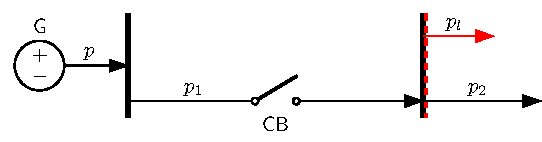
\includegraphics[height=0.13\linewidth]{figs_tikz/sl2interrupt}
\caption{Line interrupter}
\label{fig:sl2interrupt}
\end{figure}
% Figure 28:

Consider the power system shown in Figure \ref{fig:sl2interrupt} where CB denotes Circuit Breaker where $ p_l $ the loss power on the line.

If CB is closed, then, assuming negligible wire resistance, the lost power will be $ p_l \approx 0 $ and then $p_2=p_1$. But if it is open, then the output power $ p_2 $ will be zero so lost power will be $ p_l = p_1 - p_2 = p_1 $. As efficiency is
\[
\eta = \frac{p_2}{p_1}
\]
If CB is closed, it will have a value $\eta \approx 1$ and, if CB is open, it will be $ p_2 = 0 $ so $\eta=0$.

So, in order to model this element, variable $ pd $ should be an input in the model. In this way the $ pd $ value will not be given at start time, but the user will enter it at run time, similar to what occurs in actual interrupters. In this way, the efficiency value can be obtained from $ p_d $:
\[
 \eta = \frac{p_1-p_l}{p_1} = 1- \frac{p_l}{p_1} =
\begin{cases}
 \eta_1 \approx 1\; \text{if CB is closed} \\
0 \quad \text{if CB is open}
\end{cases}
\]
so an indirect way to enter the value of $\eta$, using $ p_l $ as an input, is found.

Note that, in this case the hybrid Hbus does not store energy since $p_l$ is produced by the switch.




\subsubsection{Exogenous actions}

Section \ref{interr} examined the application of System Dynamics (SD) inputs in modeling interrupters. Inputs are a subset of exogenous variables originating externally (typically from user interactions). However, a broader analysis of exogenous variables and their role in system modeling is necessary. In the context of power systems, only the power values $p_1$ and $p_2$ (measured at the left and right of a bus, respectively) can be directly observed, leading to the derivation of line power flow as $p_l=p_1-p_2$.
Smart meters can be strategically deployed along transmission lines-singly, in pairs, or at multiple locations, depending on the length and segmentation of the line. In cases where a line breaker is present, at least two smart meters should be installed to monitor and measure power flow disruptions effectively.

Smart meters, equipped with advanced communication protocols, real-time monitoring capabilities, and integrated sensors, enhance grid security and detect network attacks. Their contributions to cybersecurity in modern power grids can be categorized as follows:
\begin{enumerate}
\item Vulnerability Assessments

Smart meters can conduct proactive vulnerability assessments, identifying potential weaknesses in the network. Monitoring operational parameters helps utilities detect vulnerabilities before malicious actors can exploit them.

\item Anomaly Detection

Leveraging machine learning algorithms and pattern recognition techniques, smart meters can identify irregular behaviors in network traffic. Anomalous deviations in power consumption, voltage fluctuations, or unexpected load variations can indicate potential cyber intrusions or malicious activities.

\item Encryption and Secure Communication

Smart meters employ encryption mechanisms and secure authentication protocols to safeguard data transmission. Encryption ensures end-to-end data integrity, minimizing the risk of unauthorized interception and manipulation of critical grid information.

\item Network Segmentation and Attack Surface Reduction

The architecture of smart meter networks can be designed to operate on segmented and isolated communication infrastructures, reducing the potential attack surface. This segmentation enhances security by limiting attackers' lateral movement within the network, restricting their ability to propagate threats.

\item Intrusion Detection Systems (IDS)

Some smart meters have intrusion detection capabilities, enabling them to recognize and alert utilities about potential security incidents in real-time. These intrusion detection systems (IDS) analyze network traffic patterns and trigger alerts when deviations from normal behavior occur.

\item Proactive Monitoring and Threat Mitigation

Continuous monitoring, regular software updates, security patches, and robust vulnerability management strategies contribute to maintaining the integrity and resilience of smart meter infrastructures. By actively addressing emerging cybersecurity threats, utilities can enhance the long-term reliability and security of the smart grid.

By integrating these security-enhancing features, smart meters play a pivotal role in fortifying modern power grid infrastructures. Their ability to detect, prevent, and mitigate cyber threats enhances operational resilience and energy reliability. The increasing deployment of smart meters underscores their significance in transitioning toward secure, intelligent, and adaptive energy networks.
\end{enumerate}

By integrating these security-enhancing features, smart meters play a pivotal role in fortifying modern power grid infrastructures. Their ability to detect, prevent, and mitigate cyber threats enhances operational resilience and energy reliability. The increasing deployment of smart meters underscores their significance in transitioning toward secure, intelligent, and adaptive energy networks.


%
%Smart meters, equipped with advanced communication protocols and sensors, play
%a crucial role in identifying and detecting network attacks. Here are some ways they contribute:
%
%Vulnerability assessments: Smart meters can be used to conduct vulnerability assessments, helping to identify potential weaknesses in the network and allowing utilities to address them before attackers exploit them.
%
%Anomaly detection: Smart meters’ advanced sensors and algorithms can detect unusual patterns or behavior in network traffic, indicating potential malicious activity. Encryption and secure communication: Smart meters use encryption to protect data transmission, making it more difficult for attackers to intercept and manipulate sensitive information.
%
%Segmented networks: Smart meters can be designed to operate on isolated networks, reducing the attack surface and making it harder for attackers to move laterally within the system.
%
%Intrusion detection systems (IDS): Some smart meters are equipped with IDS capabilities, allowing them to detect and alert utilities to potential security incidents in real-time.
%
%Proactive monitoring: Regular software updates, patching, and vulnerability management ensure that smart meters remain secure and resilient against emerging threats.
%
%By incorporating these features, smart meters can help utilities and grid operators detect and respond to network attacks more effectively, ultimately enhancing the overall security and reliability of the smart grid.


\subsection{Practical Examples}

To illustrate the applicability of the methodology in modeling electrical power systems, this section presents two practical case studies: a CubeSat electrical power system (EPS) and a microgrid consisting of four residential units powered by renewable energy sources. The first example focuses on the CubeSat EPS, where SD is used to model the energy generation, storage, and consumption dynamics of a small satellite operating in orbit. This model accounts for the periodic charging of batteries via solar arrays during sunlight exposure and subsequent power distribution to onboard systems during eclipse periods. The second example explores the operation of a small-scale microgrid, integrating solar panels and a wind turbine to supply power to four houses. The SD approach allows for a detailed analysis of energy generation, load balancing, and dynamic power distribution, considering variations in renewable energy availability and household demand. These case studies demonstrate the flexibility and effectiveness of this methodology in modeling energy networks, providing insights into the performance, adaptability, and resilience of modern power systems.


But before, a basic circuit that will be a common part for any other microgrid models, is described and modeled.


\subsubsection{Basic circuit for a microgrid}

This circuit is composed by three voltage generators $v_1$, $v_2$, $v_3$,  with internal resistances $r_1$, $r_2$, $r_3$, connected in parallel to a bus (node $d$), four loads $R_1$, $R_2$, $R_3$,
$R_4$, connected in parallel to another bus (node $o$), and a transmission line with resistance $r_d$ connecting both nodes, as Figure \ref{fig:mgrid3v4r} shows.


\begin{figure}[h!]
\centering
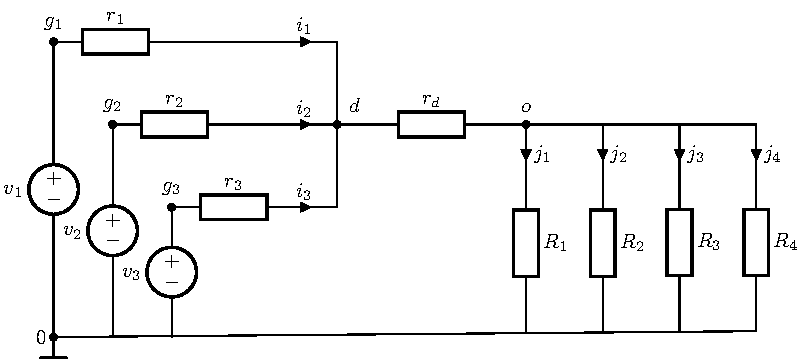
\includegraphics[width=0.7\linewidth]{figs_tikz/mgrid3v4r}
\caption{Basic circuit for a microgrid}
\label{fig:mgrid3v4r}
\end{figure}

Note that this circuit follows from the long voltage divider by replacing the  voltage generator by three ones and the load resistor by four ones.


\subsection*{SLD diagram and SD model}

The SLD of this circuit can be easily obtained from the SLD
corresponding to the LVD, by putting three generators $G_1, G_2, G_3$ in parallel instead of $G$, which inject the power flows $p_{g1}, p_{g2}, p_{g3}$, and four load resistors in parallel
$R_1, R_2, R_3, R_4 $ instead of $R$, which consume the powers $p_{l1}, p_{l2}, p_{l3}, p_{l4}$.

\begin{figure}[h]
\centering
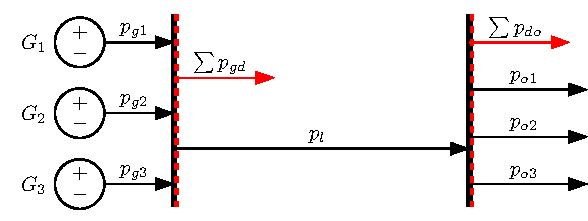
\includegraphics[width=0.5\linewidth]{figs_tikz/mgrid3v4r_sld}
\caption{SLD for the basic microgrid circuit}
\label{fig:mgrid3v4rsld}
\end{figure}



\subsubsection*{SD Model in Anylogic}
It can be easily obtained from the SD diagram of the
VD, keeping the variables $i$ and $v_o $ of that
diagram (here $v = v_o $).
\begin{figure}[h]
\centering
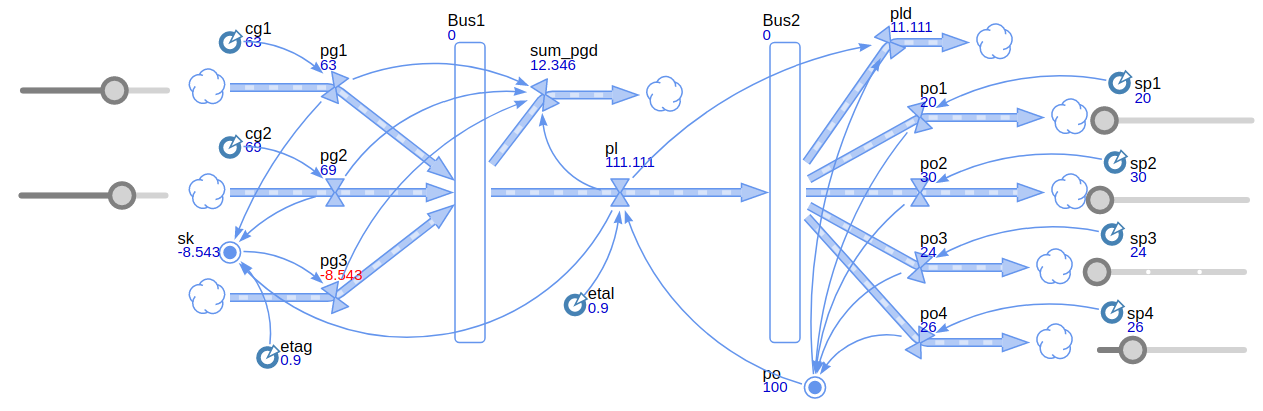
\includegraphics[width=\linewidth]{figs/al_mgrid3v4r}
\caption{AL model for the basic microgrid circuit}
\label{fig:almgrid3v4r}
\end{figure}

As in the LVD, the AL model gets from its SLD, but
conditioning each stock in SD so that $\Sigma_p = 0 $:\\
Bus2: $p_o = p_{o1} + p_{o2} + p_{o3} + p_{o4}, p_l = p_o /\eta1 p_{ld} = p_l - p_o$\\
Bus1: $s_k = p_l /\eta_2 - p_{g1} - p_{g2}, \text{sum\_pgd} = p_{g1}+p_{g2}+p_{g3}-p_l$\\
4 sliders are used to demand powers $p_{o1}, p_{o2}, p_{o3}, p_{o4}$\\
2 sliders are used to inject powers $p_{g1}$ y $p_{g2}$\\
Generator
$G_3$ is type Slack: it injects/sink the necessary power $ p_{g3} $  to fulfill $\Sigma p =0$.



\subsubsection*{Cubesat}


A CubeSat is a type of miniaturized satellite used for space research, typically built in a standardized cubic form factor. The most common size is a 1U CubeSat, which measures 10x10x10 cm and weighs about 1.33 kg, though larger configurations like 2U, 3U, or 6U are also used. CubeSats are often deployed in low Earth orbit for purposes such as Earth observation, technology demonstration, scientific experiments, and educational projects. Their compact size and relatively low cost make them accessible to universities, research institutions, and private companies.

A 1U CubeSat (10x10x10 cm) typically has the following main features, though specifics can vary depending on the mission and design:
\begin{itemize}
\item  4 to 6 solar panels, generating around 2-4 watts each

\item typically 1-2 battery packs with capacity from 10-30 Wh

\item Total power consumption from 2-10 W
\end{itemize}
\textbf{A CubeSat Electrical Power System (EPS)} is a critical subsystem responsible for generating, storing, distributing, and managing electrical power for the satellite.


Steps to Model the EPS of a CubeSat Using System Dynamics
\begin{enumerate}
\item  Define System Boundaries and Components:
\begin{itemize}
\item Subsystems: CubeSat's EPS consists of power generation (solar arrays), energy storage (batteries), and power management (distribution to payload, communications, and attitude control systems).
\item  Power Generation: Solar arrays generate power during sunlit periods, which is stored in batteries for use during eclipse periods.
\item  Energy Storage: Batteries store the excess energy generated by solar arrays and discharge energy to the CubeSat systems during power demand peaks or eclipse periods.
\end{itemize}
\item  Modeling Power Nodes as Stock Elements:
\begin{itemize}
\item  In SD, power at different points in the system (e.g., generated by solar panels, stored in batteries, and consumed by different subsystems) can be represented as stocks. These stocks represent the accumulation of power in different parts of the CubeSat.
\item  For instance, one stock could represent the energy stored in the batteries, while another stock could represent the power available for immediate consumption by the satellite's systems.
\end{itemize}
\item  Define Power Flows Between Components:
\begin{itemize}
\item  Solar Power Flow: A flow from the solar panels to the battery stock during periods of sunlight. The flow rate is determined by the solar panel's efficiency, orientation to the sun, and environmental factors.
\item  Discharge Flow: A flow from the battery to the satellite subsystems during periods of power demand, such as when the CubeSat is in eclipse or during high-power activities like image capturing and data transmission.
\item  Energy Balance: As with the paper’s DC systems model, an energy balance equation ensures that energy generated during sunlight periods meets the demands during eclipse periods.
\end{itemize}
\item  Implement Control Logic Using SD Flows:
\begin{itemize}
\item  Regulation: Use SD flow elements to model the behavior of power regulation components like DC-DC converters, ensuring that the right voltage and current are supplied to different subsystems.
\item  Power Prioritization: Certain flows can represent the priority of energy usage, ensuring that critical systems like communications or attitude control receive power before non-essential systems.
\end{itemize}
\item  Simulation of Energy Dynamics:
\begin{itemize}
\item  Orbit Cycles: The CubeSat operates in cycles of sunlight and eclipse, which can be modeled by varying the input flow of energy into the system (solar panel input) based on the CubeSat's orbital position. Eclipse times lead to increased discharge from the battery stock.
\item  Energy Dissipation: Include losses due to inefficiencies in power generation, storage, and transmission as part of the power flows.
\item  Test Scenarios for Different Operating Conditions:
\end{itemize}
\begin{itemize}
\item  High-Demand Scenarios: Model scenarios where the CubeSat is executing high-power tasks like imaging or downlinking large amounts of data. In this scenario, the discharge rate from the batteries will increase, and the model can simulate how the battery stock depletes and recharges over time.
\item  Contingency Operations: In the event of an anomaly or low-battery situation, the SD model can simulate a ``safe mode'' where only essential systems receive power, reducing the load and allowing the batteries to recharge faster.
\end{itemize}
\item  Refinement and Optimization:
\begin{itemize}
\item  Parameter Tuning: Use SD to run different simulations with varying solar panel efficiencies, battery capacities, and orbital parameters to determine the optimal EPS design that ensures continuous power availability.
\item  Energy Balance: Using System Dynamics ensures that energy is conserved within the CubeSat system, and any imbalance in power generation or consumption over time can be identified and mitigated.
\end{itemize}
\end{enumerate}

Benefits of Using System Dynamics for EPS Modeling in CubeSats
This is a comprehensive framework for modeling energy generation, storage, and consumption within the CubeSat's Electrical Power System (EPS). By ensuring that energy flows are consistent with the laws of conservation, SD enables a precise understanding of power dynamics throughout the satellite’s operational lifecycle. This approach facilitates the identification of potential energy deficits, storage limitations, and optimization opportunities, contributing to the efficient management of onboard power resources.

The modular nature of SD modeling allows for seamless scalability, enabling the extension of the CubeSat EPS model to more complex satellite configurations. Additional power subsystems, such as secondary energy storage, dynamic load balancing mechanisms, or alternative power generation sources (e.g., radioisotope thermoelectric generators for deep-space missions), can be incorporated without requiring significant model restructuring. Furthermore, SD models can be expanded to simulate multi-satellite constellations where power sharing, inter-satellite energy transfers, or collaborative power management strategies need to be considered.
SD's flexibility enables CubeSat EPS simulations under various operational scenarios, including different orbital altitudes, solar panel degradation, battery aging effects, and varying eclipse durations. This adaptability supports robust pre-deployment testing by allowing engineers to explore worst-case conditions, emergency power reallocations, and optimal energy dispatching strategies.

Beyond electrical power systems, SD modeling can be integrated with other non-electrical subsystems, such as reasoning control systems that facilitate qualitative decision-making. For instance, a high-level control layer can be added to the CubeSat model, incorporating AI-driven or rule-based decision-making frameworks to dynamically prioritize power allocation for critical subsystems. Such a system could determine when to activate or deactivate non-essential payloads, switch between primary and backup power sources, or engage emergency power-saving modes based on mission objectives and environmental conditions.

The framework supports the integration of cross-domain system models, allowing the CubeSat EPS to be connected with thermal regulation models, attitude control systems, and communication subsystems. By linking these domains, a fully dynamic and interactive simulation environment can be created, where power management strategies respond to thermal constraints, data transmission requirements, or external disturbances.


Figure \ref{fig:alcubesat} shows a power-dynamics graph of a hypothetic cubesat where for sake of simplicity only two solar panels and two loads are considered. Addition of more elements would be straightforward.

\begin{figure}[h]
\centering
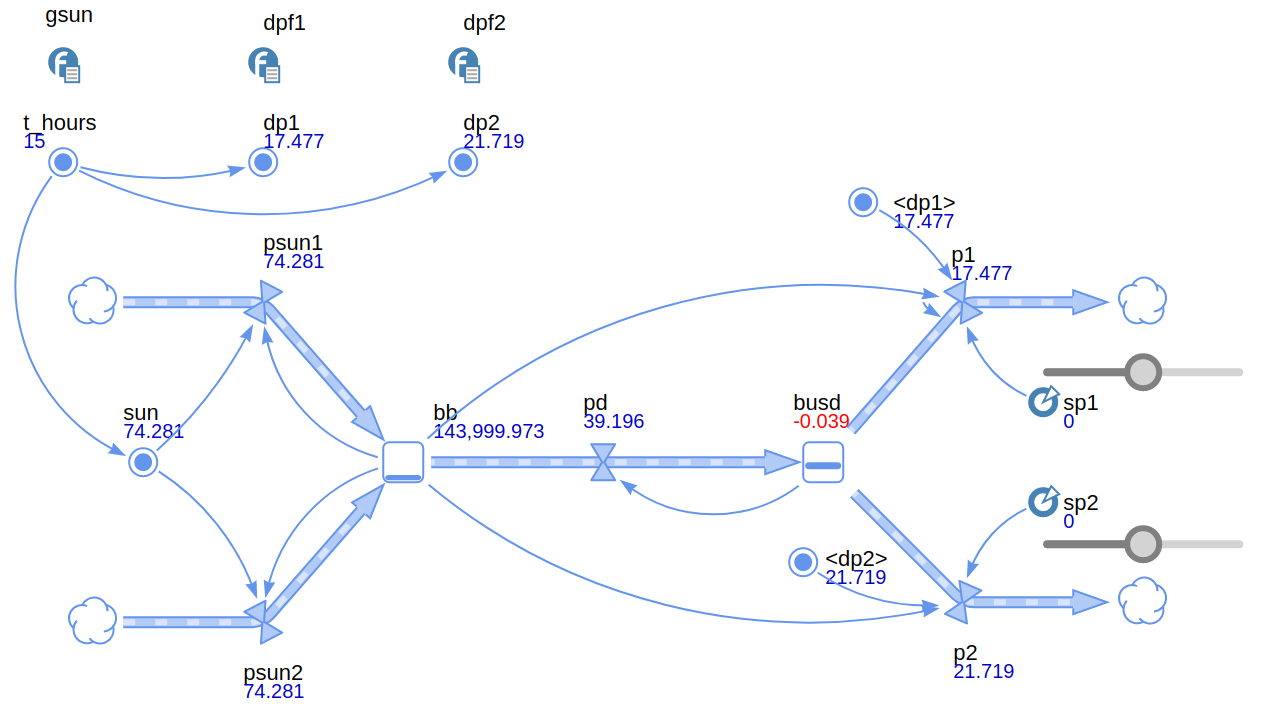
\includegraphics[width=0.7\linewidth]{figs/al_cubesat}
\caption{Cubesat EPS}
\label{fig:alcubesat}
\end{figure}


\subsubsection{Microgrid for Four Residential Units Powered by Renewable Energy Sources}
This example analyzes the dynamic modeling of a small-scale direct current (DC) microgrid, integrating localized solar panels and a wind turbine to supply power to four distinct residential houses, as depicted in the topological configuration of Figure~\ref{fig:alpf4house1}. The proposed System Dynamics (SD) approach allows for a detailed operational analysis of energy generation, load balancing, and dynamic power distribution, explicitly considering variations in renewable energy availability and household demand profile combinations.

\begin{figure}[h]
\centering
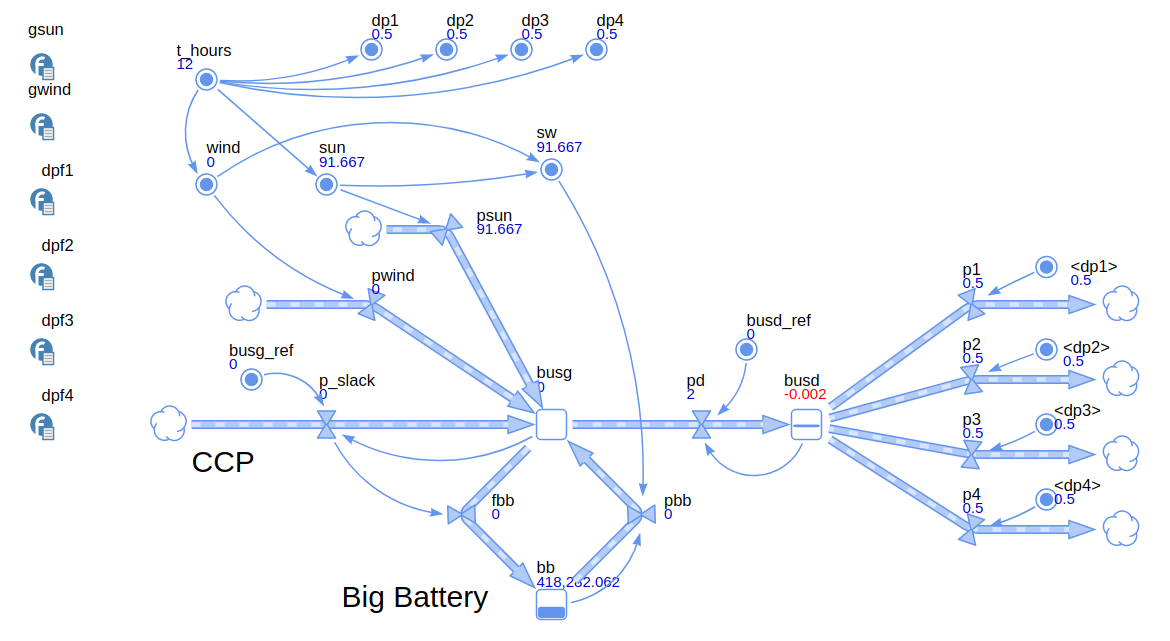
\includegraphics[width=\linewidth]{figs/al_pf4house}
\caption{AL model of a Microgrid for four households.}
\label{fig:alpf4house1}
\end{figure}

Within this AnyLogic execution environment, the \textsf{wind} and \textsf{sun} renewable generators are governed by empirical table-functions denoted as \textsf{gsun} and \textsf{gwind}, respectively. The household demand powers $p_1, p_2, p_3, p_4$ are dynamically driven by variables $d_{p1}, d_{p2}, d_{p3}, d_{p4}$, which are anchored to their respective localized consumption profiles \textsf{dpf1}, \textsf{dpf2}, \textsf{dpf3}, and \textsf{dpf4}. The aggregate magnitude of this power is absorbed directly from \textsf{busd}, which subsequently demands the net power flow \textsf{pd} through a continuous feedback loop. Concurrently, the external supply network injects through the slack channel \textsf{p\_slack} the exact necessary power flow required to maintain a strict zero energy state at \textsf{busg} via localized proportional feedback.

To manage energy surpluses, a storage system named \textsf{Big Battery} is deployed to accumulate energy whenever localized generation overflows household consumption. The simulation environment enforces the following operational constraints:
\begin{itemize}
    \item The storage device is modeled as an initially fully charged battery with a capacity of $40\,\text{Wh}$ ($144,000\,\text{J}$).
    \item The battery is charged by the incoming power flows \textsf{psun} and \textsf{pwind} until it reaches its maximum nominal saturation ceiling. Conversely, it is discharged by the net power demand flow \textsf{pd}.
    \item The power vector \textsf{pd} is demanded to the distribution bus \textsf{busd} provided that the residual battery energy satisfies the threshold condition $bb > 10,000\,\text{J}$.
    \item Specifically, individual load power $p_1$ is demanded to \textsf{busd} under the condition that the battery internal energy status satisfies $bb > 10,000\,\text{J}$.
    \item The structural power flow $p_d$ corresponding to loads $p_1, p_2, p_3, p_4$ is requested through an active feedback loop linked directly to the battery state variable \textsf{bb}.
    \item To simulate external perturbations or micro-grid human interventions, each manual interface slider can add a dynamic power variance bounded between $-10\,\text{W}$ and $+10\,\text{W}$.
\end{itemize}

From an epistemological standpoint, these case studies demonstrate the significant flexibility and effectiveness of the ``Power Dynamics'' methodology in modeling energy networks. By utilizing the Hybrid Bus (\textit{Hbus}) syntax to neutralize hardware-dependent circuit coordinates into pure power-efficiency relations, the multi-node simulation avoids the matrix inversion loops that typically slow down traditional solvers.

Furthermore, this decentralized arrangement provides critical insights into the performance, adaptability, and resilience of modern power systems. As shown by the slider-induced perturbations and the abrupt $bb$ threshold transitions, the abstract model is uniquely suited for characterizing complex environments subject to rapid discrete events, physical contingencies, or cyber-attacks (such as False Data Injection or Denial-of-Service vectors). The power-oriented syntax allows discrete-event simulators to overlay security disruptions seamlessly, tracking system-level energy deficits and wide-area resilience while completely avoiding numerical stiffness or convergence failures during severe sequence transitions. This convergence of laboratory-level telemetry and abstract graph computation successfully seals the \textit{Systematic Synthetic Identity} of the model, transforming the formal reduction into a necessary interpretation for contemporary engineering praxis.


\begin{figure}[h]
\centering
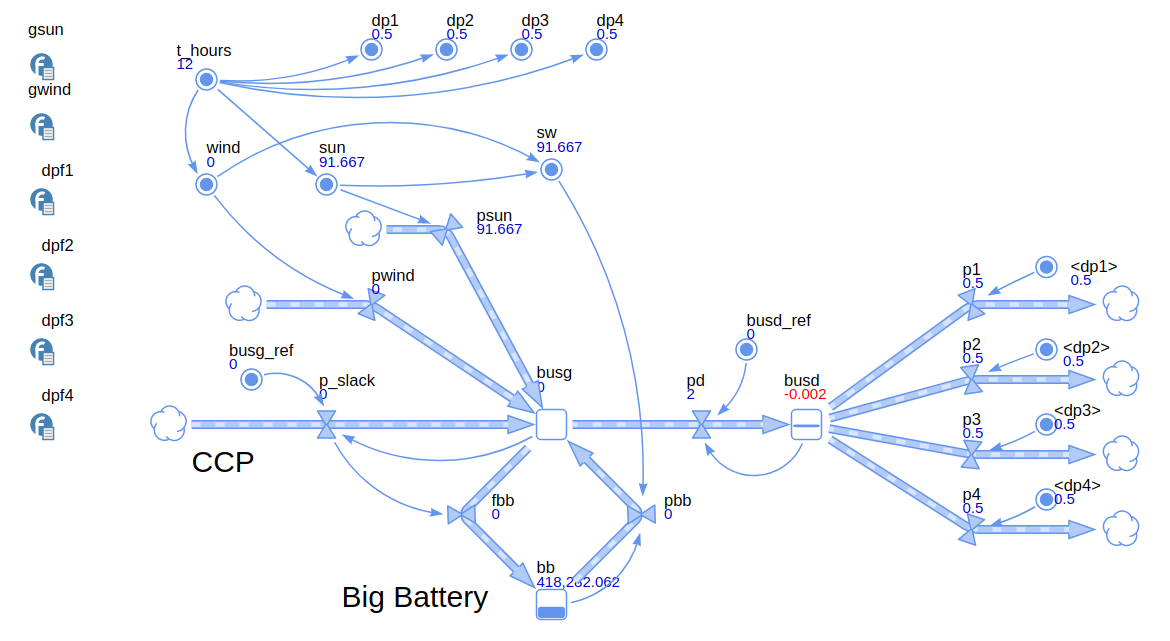
\includegraphics[width=\linewidth]{figs/al_pf4house}
\caption{AL model of a Microgrid for four households}
\label{fig:graphic_alpf4house}
\end{figure}


\subsection{Methodological capacity demonstration.}
 \label{sec:methodological_capacity}

The operational execution of the decentralized CubeSat Electrical Power System (EPS) and the four-household residential DC microgrid serves as a comprehensive, multi-scenario demonstration of the developed framework's methodological capacity. These heterogeneous implementations validate that the abstract
$(P,\eta)$ syntax is not a restrictive linear approximation, but a highly adaptive system language capable of modeling dynamic systems across diverse technological boundaries. By embedding local circuit constraints into the autonomous, first-order immanent architecture of the Hybrid Bus
($H_{bus}$), the modeling workflow achieves three significant goals: first, it filters out the high-frequency electromagnetic noise that typically triggers numerical stiffness in traditional $(V,I,R)$ DAE solvers; second, it guarantees robust global tractability during severe discrete events; and third, it provides a mathematically rigorous, device-independent platform for wide-area energy management. Ultimately, this operational demonstration bridges the historical gap between hardware-level hyperrealism and formal mathematical reductionism, successfully cementing the categorical closure of Pseudolinear Power Systems as an objective, scalable tool for modeling the smart grid and cyber-physical security issues.


\subsection{Operational advantages of the $(P, \eta)$ abstraction over traditional $(V, I, R)$ circuit models}
The first-order abstract model based on power variables and efficiency operators $(P, \eta)$ outperforms the traditional second-order circuit representation governed by voltage, current, and resistance $(V, I, R)$ when interacting with discrete-event simulators or hybrid automata \cite{gonzalezdedurana2025novel, en19020304}. This superiority is grounded on specific technical and gnoseological structural advantages detailed below:

\begin{enumerate}
    \item \textbf{Elimination of Numerical Stiffness and Convergence Failures:}
    In a standard $(V, I, R)$ configuration, the transmission lines and connections include physical lumped parameters such as loop inductances ($L$) and filter capacitances ($C$). When a discrete event occurs---such as the abrupt disconnection of a load, the isolation of a line segment by a circuit breaker, or a Denial-of-Service (DoS) cyber-attack that disables an inverter---the system variables force a state transition in zero time ($\Delta t \to 0$) \cite{moutevelis2024taxonomy, pr13092969}.
    \begin{itemize}
        \item \textbf{Within the $(V, I, R)$ framework:} This instantaneous transition forces the differential terms (such as $L \frac{di}{dt}$ and $C \frac{dv}{dt}$) to mathematically approach infinity. Numerically, the continuous integration engine faces severe numerical stiffness. The differential-algebraic equation (DAE) solver is forced to reduce its time step to fractions of a nanosecond or, under severe discontinuities, aborts the execution due to convergence failures within the Jacobian matrix \cite{en19020304, moutevelis2024taxonomy}.
        \item \textbf{Within the $(P, \eta)$ framework:} By reducing the system to a clean first-order response and absorbing the fast electromagnetic dynamics inside the efficiency operator $\eta$ (neutralizing the reactive variables at the origin, as demonstrated in Script 7), the continuous transient profiles remain smooth and free of parasitic oscillations \cite{en17143468, biom11020343}. The discrete-event simulator can jump sequentially from one timestamp contingency to another without handling mathematical infinities or stalling inside microsecond-level physical transients.
    \end{itemize}

    \item \textbf{Direct Algebraic Handling of Structural Topological Changes:}
    Contingencies involving the removal of network components or structural topology reconfigurations alter the circuit admittance matrices instantly.
    \begin{itemize}
        \item \textbf{Within the $(V, I, R)$ framework:} If a load resistance $R_2$ is disconnected, resulting in an open circuit where $R \to \infty$, the standard mesh or nodal equations collapse due to mathematical indeterminacies such as $1/R \to 0$ or $R \to \infty$. The simulation engine must halt the continuous execution, reconfigure the sparse matrix topology, and recalculate the initial boundary states from scratch.
        \item \textbf{Within the $(P, \eta)$ framework:} The interconnections are modeled as purely multiplicative and algebraic relations, matching the associative properties of the category $\mathcal{PD}$ ($\eta_{ik} = \eta_{jk} \cdot \eta_{ij}$). Removing a specific line or component reduces simply to commuting the link efficiency operator to zero ($\eta_{ij} = 0$) or deactivating the corresponding power flow $P$. The dimension of the global state space remains invariant, enabling the simulator to execute rapid contingency sequences in DC microgrids without rewriting the system matrix equations \cite{gonzalezdedurana2025novel}.
    \end{itemize}

    \item \textbf{Native Coherence with Cybersecurity and Digital Logic Layers:}
    Modern cyber-physical threats, such as False Data Injection (FDI) attacks, alongside the corrective actions executed by Energy Management Systems (EMS), operate discretely within the communication and digital power layers rather than the analog voltage or current domains \cite{pr13092969, sys12040109}.
    \begin{itemize}
        \item \textbf{Impact Mapping:} Maliciously altering an inverter power reference or blocking a battery control signal maps directly onto the abstract power graph. It changes the demanded power flow ($P$) or modifies the perceived efficiency index ($\eta$) of the hybrid bus.
        \item \textbf{Unified Interface Architecture:} The $(P, \eta)$ model provides a single native interface where the cyber-attack vector and the physical grid response share the same algebraic syntax. Conversely, evaluating the macroscopic impact of the same cyber-attack within a traditional $(V, I, R)$ model requires translating digital commands into transistor-level gate signals and solving the high-order RLC dynamics across the entire network. This hardware-level modeling quickly becomes computationally intractable for wide-area resilience assessments \cite{moutevelis2024taxonomy, pr13092969, sys12040109, appl14221111}.
    \end{itemize}
\end{enumerate}



\section{Future Plans} \label{sec:future}

We hope that future research will explore broader formal mathematical formulations for the abstract modeling introduced in this paper and extend the methodology to alternating current networks. Some possible topics for such initiatives are outlined below.

\subsection{Formalization within Category Theory} \label{sec:formalcath}

The mathematical formalization of the Hbus framework can be developed using Category Theory rather than traditional Set Theory. This choice is not arbitrary; it aligns with the epistemological foundations of Categorial Closure. While Set Theory focuses on static membership, Categorial Closure conceptualizes sciences as dynamic, operatordriven fields defined by transformations and synthetic identities among terms.  Category Theory provides the precise mathematical language required to rigorously model the operational closure and gnoseological mapping as established in the Section \ref{sec:pseudolinear}.

Gustavo Bueno was likely aware of Russell's paradox, the antinomies of Cantor's set theory, and the limitations of Hilbert's formalist program in light of Gödel's theorems \cite{godel1931}. Indeed, that famous ``foundational crisis'' in mathematics during the early 20th century is one of the historical pillars Bueno used to justify and shape his own gnoseological theory of Categorial Closure.

The power-efficiency formulations can be modeled within the framework of Category Theory to verify their structural consistency. By treating network configurations as algebraic structures, direct current (DC) power networks constitute a consistent category, can be proved. Category Theory shifts the foundational focus from objects to the arrows that relate them. This framework inherently mirrors the principles of PM Categorial Closure, where sciences are defined by transformations and synthetic identities rather than static membership.

\subsubsection{SLDs as the basis for formalization}
Single-line diagrams (SLDs) describe power networks by preserving circuit topology. A bijective correspondence exists between the physical nodes of an electrical network and the buses of an SLD, creating a direct mapping between physical components and their symbolic representations.

Our framework focuses on distribution networks. Due to their radial structures, these networks can be formulated as an interconnected system of $N$ second-order lines, resulting in a global system of order $2N$ suitable for dominant-pole reduction.

The physical space ($M_1$) connects to the abstract domain ($M_3$), mapping the RLC circuit directly onto the idealized hybrid bus (\textit{Hbus}):
\begin{equation*}
\begin{aligned}
\mathcal{M} : M_1 &\to M_3 \\
\text{RLC Circuit} &\mapsto \text{\textit{Hbus}}
\end{aligned}
\end{equation*}

This mathematical reduction is expressed via a reduction functor, $\mathcal{R}$, that establishes a structural correspondence from the Category of Power Systems (${PowSys}$) to the Category of Pseudolinear Power Systems ($PsLinPowSys$):
\begin{equation*}
\begin{aligned}
\mathcal{R} : \mathrm{PowSys} &\to \mathrm{PsLinPowSys}
\end{aligned}
\end{equation*}



\subsubsection{The Power Dynamics Category: objects and morphisms}
We define the category $\mathcal{PD}$ (Power Dynamics Category) for decentralized energy systems in steady-state operation:
\begin{itemize}
    \item {Objects ($\mathrm{Ob}(\mathcal{PD})$):} The objects represent the nodes or abstract buses of the power grid, implemented as Hybrid Buses (\textit{Hbus}). Each object $B_i$ is characterized by its power boundaries and its role in instantaneous energy balance.
    \item {Morphisms ($\mathrm{Hom}(B_i, B_j)$):} The morphisms represent the transmission lines or converters ($l_{ij}$) between buses. A morphism $f: B_i \to B_j$ is defined by the efficiency operator $\eta_{ij} \in [0, 1]$, such that:
    \begin{equation}
        P_j = \eta_{ij} \cdot P_i
    \end{equation}
\end{itemize}

\subsubsection{Axiomatic Closure and Functorial Mapping}
The category $\mathcal{PD}$ satisfies the standard algebraic axioms:
\begin{enumerate}
    \item {Identity Morphism:} For every bus $B_i$, an identity morphism $\mathrm{id}_{B_i}: B_i \to B_i$ exists with ideal efficiency $\eta_{ii} = 1$.
    \item {Composition of Morphisms:} For two cascading segments $f: B_i \to B_j$ (efficiency $\eta_{ij}$) and $g: B_j \to B_k$ (efficiency $\eta_{jk}$), their composition $(g \circ f): B_i \to B_k$ satisfies:
    \begin{equation}
        \eta_{ik} = \eta_{jk} \cdot \eta_{ij}
    \end{equation}
    This composition rule is associative, which ensures the scalability of the method for radial topologies.
\end{enumerate}

The translation from circuit variables ($V, I, R$) to System Dynamics parameters (Stocks and Flows) is modeled as a covariant functor $\mathscr{F}: \mathscr{Elec} \to \mathcal{SD}$. This functor maps the mesh equations into power-graph invariants, neutralizing hardware-dependent coordinates.



\subsection{Digital Twins for Power Flow Monitoring and Cyber-Physical Security modeling} \label{sec:future_digital_twins}

A prominent future research avenue consists in designing a lightweight, real-time Digital Twin framework specifically tailored for localized DC microgrids and distribution networks, bridging modern power grid planning through structural digital twin standards~\cite{en19020556}. Unlike traditional industrial supervisory systems—such as \textit{Siemens Spectrum Power}, which rely on high-order $(V, I, R)$ formulations that incur heavy computational overhead during massive real-time data processing and are deployed within centralized SCADA/EMS platforms to handle high-order operational optimizations~\cite{en18051020}—this proposed approach leverages the first-order $(P, \eta)$ state-space syntax to achieve ultra-scalable monitoring at the edge.

By integrating continuous telemetry streams from localized smart meters, automated algorithms would run the first-order Digital Twin in parallel as a virtual observer of the physical network. Because the abstract modeling framework filters out high-frequency electromagnetic transience, any sudden, non-topological divergence—or residual mismatch—between the physical telemetry and the twin's tracking profile could serve as an immediate diagnostic vector. Under normal operating conditions, these two independent processes converge. However, during abnormal operations, this real-time mismatch profile will be dynamically exploited not only to detect intrusions but to actively classify and isolate the specific nature of the cyber-physical threat.

Through the implementation of pattern-recognition algorithms, the framework would differentiate between material contingencies (such as conductor degradation, line faults, or terminal short circuits) and malicious network interventions, including active power theft, Denial-of-Service vectors, and stealthy False Data Injection (FDI) attacks on node telemetry. Furthermore, by exploiting the topological invariance of the Pseudolinear Power Systems category, these automated diagnostics would localize the precise geographical coordinates of the breach or contingency within the grid without incurring the computational stiffness typical of high-order differential solvers. This setup would shift the operational focus from circuit-level coordinates to System Dynamics power graphs, providing a powerful, proactive framework for wide-area energy management and microgrid security.


\subsection{Second-order matrix form and Dominant Pole reduction}
The network dynamics within the physical domain can be generalized in the classical second-order matrix differential equation as:
\begin{equation}
    M \ddot{x}(t) + B \dot{x}(t) + K x(t) = f(t)
\end{equation}
where $M$ represents the generalized inertia or mass matrix, $B$ is the damping or dissipation matrix, and $K$ is the stiffness or stiffness-equivalent coordinate matrix. This mathematical formulation is versatile and applies directly to multiple physical domains:
\begin{itemize}
    \item {Mechanical systems:} Where it models mass-spring-damper configurations under external forces.
    \item {Electrical networks:} Where it defines multi-node RLC topologies using Kirchhoff's laws.
    \item {Fluid systems:} Where it characterizes lumped-parameter hydraulic pipelines and pressure transients.
    \item {Economic systems:} Where it characterizes dynamic supply-demand interactions and market oscillations.
\end{itemize}

In large-scale microgrids or interconnected networks, the dimension $N$ of these matrices expands linearly with the number of line segments. This expansion leads to a high-dimensional state-space description that increases the computational burden in continuous-time simulators. To abstract this multidimensional second-order physical model into a simplified first-order equivalent of the form $\frac{A}{s+k}$, the framework utilizes dominant pole reduction.

The matrix differential equation is transformed into the Laplace domain via the characteristic polynomial matrix $P(s) = M s^2 + B s + K$. Under the non-oscillatory parameter constraint (overdamped regime), all system roots are real and negative. By executing a modal decomposition, the explicit state trajectory can be expressed as a linear combination of exponential decay modes:
\begin{equation}
    x(t) = \sum_{i=1}^{2N} R_i e^{s_i t}
\end{equation}
where $s_i$ are the system poles and $R_i$ represent their corresponding residue vectors.

If a specific dominant pole $s_1$ lies significantly closer to the imaginary axis than the remaining roots ($|s_1| \ll |s_i|$ for all $i \neq 1$), the high-frequency transient components associated with the faster poles decay rapidly. This timescale separation allows the systematic truncation of the fast modes, enabling the slow dominant root $s_1$ to govern the macroscopic transient response. To guarantee consistency, the inverse time constant is set as $k = |s_1|$, while the abstract gain factor $A$ is adjusted to match the static DC gain of the original second-order matrix network evaluated at $s \to 0$. This structural reduction method matches established algorithms in model order reduction (MOR) literature, validating the simplified first-order power graph as a precise tool for continuous operation.




\subsection{Gnoseological interpretation of Agent-Based Modeling paradigms}
Prior research foundations developed in \cite{durana2014agent} and \cite{durana2015agent} established multi-layered, agent-based modeling (ABM) frameworks to simulate decentralized energy networks and electric vehicle interactions. While those computational architectures successfully captured macroscopic multi-agent behaviors from a \textit{descriptionist} engineering perspective, they were formulated without an explicit epistemological grounding. Future plans involve systematically re-engineering the ABM paradigm through the concepts of Categorial Closure and Synthetic Identity from Philosophical Materialism.

Under this materialist lens, the decentralized behavioral simulation represents a dual-transit operational loop governed by statistical and structural convergence rather than deterministic curve-matching:
\begin{itemize}
\item {The gnoseological Regressus:} The analytical transit originates within the empirical, physical infrastructure of the smart grid ($M_1$), characterized by non-linear battery degradation, thermal drifts in power inverters, and stochastic consumer habits. The operating subject executes a systematic regressus by triturating these localized physical contingencies. This operation isolates the core logical grammar of each component, translating hardware constraints into deterministic, software-encoded agent behavior rules inside the formal domain ($M_3$).

\item {The gnoseological Progressus:} Once the rule-sets of the individual agents are stabilized in the computational plane ($M_3$), the simulation executes their collective, massive interaction over time. The progressus represents the return path toward the material domain ($M_1$), where these local algorithmic rules force the emergence of macro-level grid phenomena, such as aggregated load profiles, synchronization boundaries, and network power flow distributions.

\item {The Categorial Closure via statistical identities:} Unlike the exact geometric curve-fitting achieved in the dominant-pole reduction of transmission lines, the closure within the ABM paradigm should be structural and statistical.

The verification of the \textit{Systematic Synthetic Identity} would be established by defining macroscopic and topological metrics---such as probability density functions of demand peaks, variance thresholds, and spectral densities of grid frequency fluctuations.

When the statistical invariants computed from the emergent multi-agent interactions ($M_3$) match the empirical telemetry gathered by smart meters in the real grid ($M_1$), a gnoseological closure is achieved. The abstract logical rules are validated because they successfully govern and predict the macroscopic, stochastic reality of the physical energy infrastructure.
\end{itemize}

This future research line aims to determine how the decentralized multi-agent simulations match the syntax of physical circuits, transforming descriptive agent parameters into useful norms for energy management.

%\section*{Appendices}


% =====================================================================
% APPENDIX A: DEFINITIVE UNIFIED SUITE OF PYTHON SCRIPTS (1-7)
% =====================================================================
\appendix \setcounter{section}{0}

%\section[Python Scripts]{\protect\linebreak \\ Python Scripts}

\section{Python Scripts}

This appendix aggregates the complete suite of simulation scripts developed across the review paper to validate the abstract modeling workflows. All codes have been verified under Python 3.13 and NumPy 2.0+.


\subsection*{Script 1: Step response of output voltage $v_3(t)$}
This script computes the second-order step response under a constant load resistance ($R_2 = 100\,\Omega$) using zero initial conditions.

{\footnotesize

\begin{verbatim}
import numpy as np
import matplotlib.pyplot as plt
from scipy.integrate import solve_ivp

V_1, R1, L1, C1, R2 = 12.0, 10.0, 0.001, 0.0001, 100.0

def circuit_dynamics(t, x):
    v3, i_L = x[0], x[1]
    dv3_dt = (i_L - v3 / R2) / C1
    di_L_dt = (V_1 - R1 * i_L - v3) / L1
    return [dv3_dt, di_L_dt]

x0 = [0.0, 0.0]
t_span = (0, 0.01)
t_eval = np.linspace(t_span[0], t_span[1], 1000)
sol = solve_ivp(circuit_dynamics, t_span, x0, t_eval=t_eval, method='Radau')

plt.figure(figsize=(8, 4))
plt.plot(sol.t * 1000, sol.y[0], 'b-', label=r'$v_3(t)$')
plt.title('Case 1: Step Response of the Output Voltage $v_3(t)$')
plt.xlabel('Time (ms)')
plt.ylabel('Voltage (V)')
plt.grid(True)
plt.legend()
plt.savefig('script1.pdf', format='pdf', bbox_inches='tight')
plt.show()
\end{verbatim}
}


\subsection*{Script 2: Voltage response under resistance change at $t=4$ ms}
This script introduces an abrupt step-change in the load resistance ($R_2$ dropping to half) at an arbitrary transient threshold, tracking the continuous state-space trajectory.

{\footnotesize
\begin{verbatim}
import numpy as np
import matplotlib.pyplot as plt
from scipy.integrate import solve_ivp

V_1, R1, L1, C1, R2_initial, t_switch = 12.0, 10.0, 0.001, 0.0001, 100.0, 0.004

def circuit_dynamics_dynamic(t, x):
    v3, i_L = x[0], x[1]
    R2 = R2_initial if t < t_switch else (R2_initial / 2.0)
    dv3_dt = (i_L - v3 / R2) / C1
    di_L_dt = (V_1 - R1 * i_L - v3) / L1
    return [dv3_dt, di_L_dt]

x0 = [0.0, 0.0]
t_span = (0, 0.01)
t_eval = np.linspace(t_span[0], t_span[1], 1000)
sol = solve_ivp(circuit_dynamics_dynamic, t_span, x0, t_eval=t_eval, method='Radau', max_step=1e-5)

plt.figure(figsize=(8, 4))
plt.plot(sol.t * 1000, sol.y[0], 'r-', label=r'$v_3(t)$')
plt.axvline(x=t_switch*1000, color='k', linestyle='--', label='$R_2$ Change')
plt.title('Case 2: Response under Resistance Variation in $R_2$')
plt.xlabel('Time (ms)')
plt.ylabel('Voltage (V)')
plt.grid(True)
plt.legend()
plt.savefig('script2.pdf', format='pdf', bbox_inches='tight')
plt.show()
\end{verbatim}
}


Script 3: Source and load powers under step input
Script 4: Power flows under load switching at $t=4$ ms
Script 5: Load swithing mapped to the origin ($t=0$)
Script 6: Transient power transition mapped at the origin ($t=0$)
Script 7: Dominant pole optimization and Synthetic Identity calibration
Script 8: Parametric mapping and boundaries of the valid cables collection

\subsection*{Script 3: Source and load powers under step input}
This script computes the instantaneous active power flow delivered by the source ($p_{gen}$) and the power absorbed by the load ($p_{R2}$), after a step $V_1$ is applied to the input.

{\footnotesize
\begin{verbatim}
import numpy as np
import matplotlib.pyplot as plt
from scipy.integrate import solve_ivp

V_1, R1, L1, C1, R2 = 12.0, 10.0, 0.001, 0.0001, 100.0

def circuit_dynamics(t, x):
    v3, i_L = x[0], x[1]
    dv3_dt = (i_L - v3 / R2) / C1
    di_L_dt = (V_1 - R1 * i_L - v3) / L1
    return [dv3_dt, di_L_dt]

x0 = [0.0, 0.0]
t_span = (0, 0.01)
t_eval = np.linspace(t_span[0], t_span[1], 1000)
sol = solve_ivp(circuit_dynamics, t_span, x0, t_eval=t_eval, method='Radau')

p_total = V_1 * sol.y[1]
p_R2 = (sol.y[0] ** 2) / R2

plt.figure(figsize=(8, 4))
plt.plot(sol.t * 1000, p_total, 'g-', label=r'Total Supplied Power ($p_{gen}$)')
plt.plot(sol.t * 1000, p_R2, 'm-', label=r'Load Power ($p_{R2}$)')
plt.title('Case 1: Transient Power Evaluation')
plt.xlabel('Time (ms)')
plt.ylabel('Power (W)')
plt.grid(True)
plt.legend()
plt.savefig('script3.pdf', format='pdf', bbox_inches='tight')
plt.show()
\end{verbatim}
}



\subsection*{Script 4: Power flows under load switching at $t=4$ ms}
This script highlights the power mismatch and the abrupt vertical jump experienced by the load power profile during dynamic impedance shifting.

{\footnotesize
\begin{verbatim}
import numpy as np
import matplotlib.pyplot as plt
from scipy.integrate import solve_ivp

V_1, R1, L1, C1, R2_initial, t_switch = 12.0, 10.0, 0.001, 0.0001, 100.0, 0.004

def circuit_dynamics_dynamic(t, x):
    v3, i_L = x
    R2 = R2_initial if t < t_switch else (R2_initial / 2.0)
    dv3_dt = (i_L - v3 / R2) / C1
    di_L_dt = (V_1 - R1 * i_L - v3) / L1
    return [dv3_dt, di_L_dt]

x0 = [0.0, 0.0]
t_span = (0, 0.01)
t_eval = np.linspace(0, 0.01, 1000)
sol = solve_ivp(circuit_dynamics_dynamic, t_span, x0, t_eval=t_eval, method='Radau', max_step=1e-5)

v3, i_L = sol.y
R2_array = np.where(sol.t < t_switch, R2_initial, R2_initial / 2.0)
p_total = V_1 * i_L
p_R2 = (v3 ** 2) / R2_array

plt.figure(figsize=(8, 4))
plt.plot(sol.t * 1000, p_total, 'g-', label=r'Total Supplied Power ($p_{gen}$)')
plt.plot(sol.t * 1000, p_R2, 'm-', label=r'Load Power ($p_{R2}$)')
plt.axvline(x=t_switch*1000, color='k', linestyle='--', label='$R_2$ Change')
plt.title('Case 2: Power Evaluation under Resistance Variation')
plt.xlabel('Time (ms)')
plt.ylabel('Power (W)')
plt.grid(True)
plt.legend()
plt.savefig('script4.pdf', format='pdf', bbox_inches='tight')
plt.show()
\end{verbatim}
}




\subsection*{Script 5: Load swithing mapped to the origin ($t=0$)}
This script shifts the topological transition precisely to $t=0^+$ by configuring the steady-state pre-conmutation coordinates as the vector $x_0$, isolating the dynamic response.

{\footnotesize
\begin{verbatim}
import numpy as np
import matplotlib.pyplot as plt
from scipy.integrate import solve_ivp

V_1, R1, L1, C1, R2_initial, R2_final = 12.0, 10.0, 0.001, 0.0001, 100.0, 50.0

v3_0 = (R2_initial / (R1 + R2_initial)) * V_1
iL_0 = V_1 / (R1 + R2_initial)
x0 = [v3_0, iL_0]

def circuit_dynamics_after_switch(t, x):
    v3, i_L = x, x
    dv3_dt = (i_L - v3 / R2_final) / C1
    di_L_dt = (V_1 - R1 * i_L - v3) / L1
    return [dv3_dt, di_L_dt]

t_span = (0, 0.006)
t_eval = np.linspace(t_span[0], t_span[1], 1000)
sol = solve_ivp(circuit_dynamics_after_switch, t_span, x0, t_eval=t_eval, method='Radau')

t_ms = sol.t * 1000
p_total = V_1 * sol.y[1]
p_R2 = (sol.y[0] ** 2) / R2_final

fig, ax = plt.subplots(figsize=(8, 4.5))
ax.plot(t_ms, p_total, 'g-', lw=2, label=r'Total Source Power ($p_{gen}$)')
ax.plot(t_ms, p_R2, 'm-', lw=2, label=r'Load Power ($p_{R2}$)')
ax.set_xlabel('Time (ms)')
ax.set_ylabel('Power (W)')
ax.set_title('Transient Power Evaluation (Shifted to Origin)')
ax.grid(True, linestyle='--', alpha=0.7)
ax.legend(loc='upper right')
plt.tight_layout()
plt.savefig('script6_powers_origin.pdf', format='pdf', bbox_inches='tight')
plt.show()
\end{verbatim}
}


\subsection*{Script 6: Transient power transition mapped at the origin ($t=0$)}
The following script solves the Dynamic State Model (DSM) by setting the steady-state pre-switching conditions as the initial vector $x_0$, shifting the load conmutation threshold precisely to the mathematical origin.

{\footnotesize
\begin{verbatim}
import numpy as np
import matplotlib.pyplot as plt
from scipy.integrate import solve_ivp

# Circuit parameters and initial conditions (t = 0-)
V_1 = 12.0
R1 = 10.0
L1 = 0.001
C1 = 0.0001
R2_initial = 100.0
R2_final = 50.0

# Steady-state initial conditions just before switching (t=0-)
v3_0 = (R2_initial / (R1 + R2_initial)) * V_1
iL_0 = V_1 / (R1 + R2_initial)
x0 = [v3_0, iL_0]

# Circuit dynamics after switching (t >= 0)
def circuit_dynamics_after_switch(t, x):
    v3, i_L = x[0], x[1]
    dv3_dt = (i_L - v3 / R2_final) / C1
    di_L_dt = (V_1 - R1 * i_L - v3) / L1
    return [dv3_dt, di_L_dt]

# Simulation execution (0 to 6 milliseconds)
t_span = (0, 0.006)
t_eval = np.linspace(t_span[0], t_span[1], 1000)
sol = solve_ivp(circuit_dynamics_after_switch, t_span, x0, t_eval=t_eval, method='Radau')

# Data extraction and transient power flow synthesis
t_ms = sol.t * 1000
p_total = V_1 * sol.y[1]
p_R2 = (sol.y[0] ** 2) / R2_final

# Scientific layout visualization
fig, ax = plt.subplots(figsize=(8, 4.5))
ax.plot(t_ms, p_total, 'g-', lw=2, label='Total Source Power ($p_{gen}$)')
ax.plot(t_ms, p_R2, 'm-', lw=2, label='Load Power ($p_{R2}$)')
ax.set_xlabel('Time (ms)')
ax.set_ylabel('Power (W)')
ax.set_title('Transient Power Evaluation (Shifted to Origin)')
ax.grid(True, linestyle='--', alpha=0.7)
ax.legend(loc='upper right')
plt.tight_layout()
plt.savefig('script6_powers_origin.pdf', format='pdf', bbox_inches='tight')
plt.show()
\end{verbatim}
}


\subsection*{Script 7: Dominant pole optimization and Synthetic Identity calibration}
This final script evaluates the metric convergence (IAPE) between the real ($M_1$) and abstract ($M_3$) power flows, sealing the Systematic Synthetic Identity closure.

{\footnotesize
\begin{verbatim}
import numpy as np
import matplotlib.pyplot as plt
from scipy.integrate import solve_ivp

V_1, R1, L1, C1, R2_initial, R2_final = 12.0, 10.0, 0.001, 0.0001, 100.0, 50.0

v3_0 = (R2_initial / (R1 + R2_initial)) * V_1
iL_0 = V_1 / (R1 + R2_initial)
x0 = [v3_0, iL_0]

def circuit_dynamics_after_switch(t, x):
    v3, i_L = x, x
    dv3_dt = (i_L - v3 / R2_final) / C1
    di_L_dt = (V_1 - R1 * i_L - v3) / L1
    return [dv3_dt, di_L_dt]

t_span = (0, 0.006)
t_eval = np.linspace(t_span[0], t_span[1], 1500)
sol_m2 = solve_ivp(circuit_dynamics_after_switch, t_span, x0, t_eval=t_eval, method='Radau')

t_ms = sol_m2.t * 1000
v3_m2 = sol_m2.y[0]
p_R2_m2 = (v3_m2 ** 2) / R2_final

alpha = 0.5 * (R1/L1 + 1/(R2_final*C1))
omega_0_sq = (R1 + R2_final) / (R2_final * L1 * C1)
s1 = -alpha + np.sqrt(alpha**2 - omega_0_sq)
k_abstract = abs(s1)
v3_inf = (R2_final / (R1 + R2_final)) * V_1
A_abstract = v3_inf * k_abstract

v3_m1 = v3_inf + (v3_0 - v3_inf) * np.exp(-k_abstract * sol_m2.t)
p_R2_m1 = (v3_m1 ** 2) / R2_final

def modern_trapz(y, x):
    return np.sum((y[1:] + y[:-1]) * np.diff(x)) / 2.0

iape_energy_error = modern_trapz(np.abs(p_R2_m2 - p_R2_m1), sol_m2.t)
relative_error_pct = (iape_energy_error / modern_trapz(p_R2_m2, sol_m2.t)) * 100

print(``========================================================='')
print(f``Dominant Pole (k): {k_abstract:.2f} rad/s'')
print(f``Abstract Gain Factor (A): {A_abstract:.2f} V/s'')
print(f``IAPE Energy Error: {iape_energy_error*1000:.4f} mJ'')
print(f``Relative Mismatch Profile: {relative_error_pct:.4f} %'')
print(``========================================================='')

fig, (ax1, ax2) = plt.subplots(2, 1, figsize=(8, 7), sharex=True)
ax1.plot(t_ms, v3_m2, 'b-', lw=2.5, label=r'Real $2^{\mathrm{nd}}$-Order Voltage ($M_1$)')
ax1.plot(t_ms, v3_m1, 'r--', lw=2, label=r'Abstract $1^{\mathrm{st}}$-Order Voltage ($M_3$)')
ax1.set_ylabel('Voltage $v_3(t)$ (V)')
ax1.set_title('Voltage State Space Trajectory Comparison')
ax1.grid(True, linestyle=':', alpha=0.6)
ax1.legend(loc='lower right')

ax2.plot(t_ms, p_R2_m2, 'm-', lw=2.5, label='Real Load Power ($M_1$)')
ax2.plot(t_ms, p_R2_m1, 'c--', lw=2, label='Abstract Load Power ($M_3$)')
ax2.fill_between(t_ms, p_R2_m2, p_R2_m1, color='gray', alpha=0.2, label='Energy Error Area')
ax2.set_xlabel('Time (ms)')
ax2.set_ylabel('Power $p_{R2}(t)$ (W)')
\end{verbatim}
}


\subsection*{Python Scripts for transient terification and Gnoseological Closure}
This appendix provides the core Python implementation utilized across this review paper to validate the abstract modeling workflows. To guarantee structural stability and compliance with modern software ecosystems (tested under Python 3.13 and NumPy 2.0+), all scripts avoid deprecated integration namespaces and leverage raw string notation to prevent LaTeX rendering conflicts during data plotting.


\subsection*{Script 8: Parametric mapping and boundaries of the valid cables collection} \label{app:script8}
The following script executes the quantitative sweep across the parametric design space of commercial cables. By systematically evaluating the second-order characteristic discriminant and the separation of time scales ($\sigma = |s_2 / s_1| \ge 5.0$), this code isolates the geometric boundaries in the $M_3$ domain where the first-order Power Dynamics model accurately mirrors the macroscopic physical transients.

{\footnotesize
\begin{verbatim}
# =====================================================================
# Script 8: Geometric Mapping of Valid Commercial Cables Suite
# Author: José González de Durana
# Article: Abstract modeling: formal reduction to praxis interpretation
# Environment: Python 3.13 / NumPy 2.0+ Compliant
# =====================================================================
import numpy as np
import matplotlib.pyplot as plt

# 1. FIXED NETWORK CONFIGURATION (M1 Operational Layer)
V_s = 12.0
R2_nominal = 50.0  # Nominal load resistance (from Script 7 final state)

# Cable baseline parameters per kilometer (typical commercial microgrid values)
R_per_km = 0.50     # Ohms/km
L_per_km = 150e-6   # Henries/km

# 2. PARAMETER SPACE RESOLUTION (Grid Definition)
lengths = np.linspace(0.1, 5.0, 400)      # Line length from 100m to 5km
capacitances = np.linspace(1e-6, 500e-6, 400) # Filter capacity from 1uF to 500uF

# Create 2D mesh grid
Length_Grid, C1_Grid = np.meshgrid(lengths, capacitances)

# Calculate localized lumped parameters across the grid
R1_Grid = Length_Grid * R_per_km
L1_Grid = Length_Grid * L_per_km

# 3. SECOND-ORDER CHARACTERISTIC EVALUATION & TIMESCALE SEPARATION
# Alpha (attenuation factor) and Omega_0 squared (undamped natural frequency)
alpha = 0.5 * (R1_Grid / L1_Grid + 1.0 / (R2_nominal * C1_Grid))
omega_0_sq = (R1_Grid + R2_nominal) / (R2_nominal * L1_Grid * C1_Grid)

# Discriminant array for overdamped regime validation
discriminant = alpha**2 - omega_0_sq

# Isolate real roots across the parametric mesh
s1 = -alpha + np.sqrt(np.maximum(0, discriminant)) # Slower dominant pole
s2 = -alpha - np.sqrt(np.maximum(0, discriminant)) # Faster pole

# Define validation criteria filters
is_overdamped = discriminant > 0
timescale_separation = np.abs(s2 / s1) >= 5.0 # Strict factor of 5 separation

# Combine masks into the definitive ``Valid Cable'' domain matrix
valid_cables_mask = is_overdamped & timescale_separation

# 4. SCIENTIFIC VISUALIZATION (MDPI ENERGIES GEOMETRIC LAYOUT)
plt.figure(figsize=(8.5, 6))

# Plot the parametric design domains using filled contours
cp = plt.contourf(Length_Grid, C1_Grid * 1e6, valid_cables_mask.astype(int),
                  levels=[-0.5, 0.5, 1.5],
                  colors=['#f8d7da', '#d4edda'], alpha=0.9)

# Overlay the explicit boundaries
plt.contour(Length_Grid, C1_Grid * 1e6, discriminant, levels=[0],
            colors=['red'], linewidths=2.0, linestyles='--')

# Plot labels and architectural styling
plt.title(r'Geometric Boundaries of the ``Valid Cables Collection'' ($M_3$ Design Space)', fontsize=12, pad=15)
plt.xlabel('Cable Length (km)', fontsize=10)
plt.ylabel(r'Filter Capacitance $C_1$ ($\mu$F)', fontsize=10)

# Visual anchors (custom annotations for the chart)
plt.text(1.0, 100, 'VALID COLLECTION\n(First-Order Abstraction\nMatches Real Transient)',
         color='green', fontsize=10, weight='bold', ha='center', bbox=dict(facecolor='white', alpha=0.7, boxstyle='round,pad=0.5'))

plt.text(3.5, 400, 'INVALID ZONE\n(Oscillatory or Non-Dominant\nSecond-Order Dynamics)',
         color='darkred', fontsize=10, weight='bold', ha='center', bbox=dict(facecolor='white', alpha=0.7, boxstyle='round,pad=0.5'))

# Overlay line marking the Overdamped exact border for the paper
proxy_line = plt.Line2D([0], [0], color='red', linestyle='--', lw=2, label=r'Overdamped Boundary ($\alpha^2 = \omega_0^2$)')
plt.legend(handles=[proxy_line], loc='upper right')

plt.grid(True, linestyle=':', alpha=0.5)
plt.tight_layout()
plt.savefig('script8_valid_cables_map.pdf', format='pdf', bbox_inches='tight')
plt.show()
\end{verbatim}
}


% =====================================================================
% MDPI ENERGIES - BACK MATTER BLOCK
% =====================================================================
%\section*{Supplementary Materials}
%The complete suite of Python simulation scripts developed for this research---including Script 1 (Step Response), Script 2 (Dynamic Resistance Switching at $t=4\,\mathrm{ms}$), Script 3 (Transient Power Evaluation), and Script 4 (Dynamic Power Flows under Parameter Variation)---is available in the following GitHub repository: \url{https://github.com/jmgdurana}. These materials are provided to ensure full computational reproducibility and to serve as an open-source benchmark for abstract modeling in direct current (DC) power system control.


{\color{red} GitHub}

\section*{Supplementary Materials}
The complete suite of Python scripts and AnyLogic source architectures developed for this research is available online at the GitHub repository\;  \url{https://github.com/jmgdurana}\\
This open-source benchmark includes:
\begin{itemize}
\item {Python suite:}
Script 1 (Step response of output voltage $v_3(t)$),
Script 2 (Voltage response under resistance change at $t=4$ ms),
Script 3 (Source and load powers under step input),
Script 4 (Power flows under load switching at $t=4$ ms),
Script 5 (Load swithing mapped to the origin ($t=0$)),
Script 6 (Transient power transition mapped at the origin ($t=0$)),
Script 7 (Dominant pole optimization and Synthetic Identity calibration) and
Script 8 (Parametric mapping and boundaries of the valid cables collection)
 to evaluate the steady-state and dynamic behavior of Pseudolinear Power Systems.
    \item {AnyLogic source files:} The complete simulation models (\textit{.alp} format) materializing the Hybrid Bus (\textit{Hbus}) operational nodes, categorical closure boundaries, and multi-agent state-charts.
\end{itemize}



These computational materials are provided to ensure full reproducibility, serving as an open-source validation platform to test artificial intelligence frameworks, energy storage scheduling algorithms, and proactive ciber-physical anomaly detection methods in modern smart grids.


\section*{Acknowledgments}
The author wishes to express his sincere gratitude to his colleagues and research collaborators at the University of Central Florida (UCF) for their insightful comments, technical discussions, and enriching feedback throughout the development of this work. Additionally, the author acknowledges the computational and grammatical assistance provided by Google's artificial intelligence (AI) models, which served as an advanced support tool for optimizing the implementation of the simulation scripts and refining the textual and stylistic framework of several theoretical sections within this comprehensive review.


\bibliographystyle{plain}
\bibliography{abstract_systems}


\end{document}

